\chapter[Số tự nhiên, Số nguyên và Số hữu tỉ]{Số tự nhiên, Số nguyên và Số hữu tỉ\footnote{Nội dung chương này được sắp xếp theo tinh thần của phương pháp tiên đề. Bạn đọc nên tập trung vào các kết quả và trình tự của tất cả trước thay vì đọc các chứng minh chi tiết ngay từ đầu.}}\label{chapter:natural-numbers-integers-and-rationals}

\noindent ``God made the natural numbers; all else is the work of man.\@''

\noindent \rule[0.5ex]{2cm}{0.5pt}

\noindent \textit{Leopold Kronecker ($1823-1891$)}

\section{Số tự nhiên}\label{section:natural-numbers}

\subsection*{Hệ tiên đề Peano}

Cuối thế kỉ 19, nhà toán học người Ý Giuseppe Peano đưa ra một hệ tiên đề về các số tự nhiên. Hệ tiên đề này gồm 9 tiên đề sau.

\begin{axiom}
	$0$ và $S$ là hai đối tượng không được định nghĩa.

	\begin{enumerate}[label={(PA\arabic*)},itemsep=0pt,topsep=0pt,itemindent=0.25cm]
		\item $0$ là một số tự nhiên.
		\item Với mọi số tự nhiên $x$, có $x = x$.
		\item Với mọi số tự nhiên $x$ và $y$, nếu $x = y$ thì $y = x$.
		\item Với mọi số tự nhiên $x, y$, và $z$, nếu $x = y$ và $y = z$ thì $x = z$.
		\item Với mọi $x$ và $y$, nếu $y$ là số tự nhiên và $x = y$ thì $x$ cũng là một số tự nhiên.
		\item Với mọi số tự nhiên $x$, $S(x)$ là một số tự nhiên.
		\item Với mọi số tự nhiên $x$ và $y$, nếu $S(x) = S(y)$ thì $x = y$.
		\item Với mọi số tự nhiên $x$, $S(x) \ne 0$.
		\item Nếu một tập hợp $A$ thỏa mãn hai điều kiện sau
		      \begin{itemize}[itemsep=0pt,topsep=0pt]
			      \item $0\in A$,
			      \item với mọi số tự nhiên $n$, $n\in A$ kéo theo $S(n)\in A$,
		      \end{itemize}
		      thì mọi số tự nhiên đều thuộc $A$.
	\end{enumerate}
\end{axiom}

Tập hợp (tất cả) các số tự nhiên được kí hiệu là $\mathbb{N}$.

Tiên đề 1 khẳng định tập hợp số tự nhiên không rỗng. Hệ tiên đề ban đầu của Peano chọn $1$ làm số tự nhiên ``đầu tiên'' thay vì $0$. Nhưng trong tác phẩm chính thức của mình, ông lại chọn số $0$ làm số tự nhiên đầu tiên. Cho đến nay, cộng đồng toán học không thống nhất rằng $0$ là số tự nhiên hay không $-$ Đây chỉ là vấn đề quy ước. Vì sự nhập nhằng đó, thay vì viết là ``số tự nhiên'', nhiều tác giả chọn cách viết là ``số nguyên dương'', ``số nguyên không âm''.

Tiên đề 2, 3, 4, 5 nói về quan hệ bằng nhau trên tập hợp số tự nhiên. Ba tiên đề 2, 3, 4 khẳng định quan hệ bằng nhau trên tập hợp số tự nhiên là một quan hệ tương đương. Tiên đề 5 có nghĩa là tập hợp số tự nhiên là \textit{đóng} dưới quan hệ bằng nhau (một số tự nhiên không thể bằng một đối tượng nào đó nằm ngoài tập hợp số tự nhiên).

Đối tượng $S$ không được định nghĩa trong hệ tiên đề trên. $S$ được gọi là hàm successor (có nghĩa là kế tiếp, chúng tôi không dùng tên gọi được dịch). Tiên đề 6 phát biểu rằng tập hợp số tự nhiên đóng dưới hàm successor. Tiên đề 7 có nghĩa là $S$ là một đơn ánh. Tiên đề 8 có nghĩa là không có số tự nhiên nào nhận $0$ làm số tự nhiên liền sau nó. Ý nghĩa của hàm successor là nó gán một số tự nhiên với số tự nhiên ngay kế tiếp.

Tiên đề 9 chính là nguyên lý quy nạp toán học. Tiên đề 9 còn được gọi là \textit{tiên đề quy nạp}.

Ở mục tiếp theo, chúng ta sẽ định nghĩa phép cộng, phép nhân, quan hệ thứ tự trên tập hợp số tự nhiên, và chứng minh nhiều tính chất của chúng. Bên cạnh 9 tiên đề Peano, hai công cụ duy nhất chúng ta có là phương pháp phản chứng và phương pháp quy nạp toán học. Do đó, ở hai mục tiếp theo, phương pháp quy nạp toán học sẽ được áp dụng triệt để. Dưới đây là chứng minh cho nguyên lý quy nạp toán học.

Chúng ta nhắc lại nội dung nguyên lý quy nạp toán học: Nếu hai điều kiện sau thỏa mãn
\begin{enumerate}[label={(\roman*)}]
	\item mệnh đề $p(0)$ đúng,
	\item với mọi số tự nhiên $k\geq 0$, $p(k)$ kéo theo $p(k+1)$,
\end{enumerate}

thì $p(n)$ đúng với mọi số tự nhiên $n$.

\begin{proof}[Chứng minh nguyên lý quy nạp toán học]
	Chúng ta gọi $A$ là tập hợp các số tự nhiên $n$ sao cho có $p(n)$.

	Vì có $p(0)$ nên $0\in A$.

	Vì với mọi số tự nhiên $k\geq 1$, $p(k)$ kéo theo $p(k+1)$ nên với mọi số tự nhiên $k\geq 1$, $k\in A$ kéo theo $(k+1)\in A$.

	Theo tiên đề 9, $A$ chứa mọi số tự nhiên. Theo định nghĩa của tập hợp $A$, có $p(n)$ với mọi số tự nhiên $n$.
\end{proof}

Có thể bạn đọc đã bỏ qua một câu hỏi: ``Ngoài $0$, còn số tự nhiên $n$ nào mà không tồn tại số tự nhiên $m$ sao cho $S(m) = n$ không?\@'' Câu trả lời là không. Nhưng chúng ta cần một chứng minh.
\begin{theorem}\label{theorem:successor}
	Nếu $n$ là một số tự nhiên khác $0$ thì tồn tại một số tự nhiên $m$ sao cho $S(m) = n$.
\end{theorem}

\begin{proof}
	Mệnh đề có phát biểu tương đương như sau: Với mọi số tự nhiên $n$, nếu $n$ khác $0$ thì tồn tại số tự nhiên $m$ sao cho $S(m) = n$.

	Khi $n = 0$, tức là mệnh đề $n$ là số tự nhiên khác $0$ sai, thì theo tiên đề 8 không có số tự nhiên $m$ nào sao cho $S(m) = n$ (lưu ý rằng mệnh đề kéo theo $P\implies Q$ đúng khi $P$ và $Q$ sai).

	Khi $n = 1$, chúng ta có $S(0) = 1$.

	Giả sử với số tự nhiên $k\geq 1$, $n = k$ kéo theo tồn tại số tự nhiên $m$ sao cho $S(m) = k$. Khi đó $S(S(m)) = S(k)$.

	Theo nguyên lý quy nạp toán học, với mọi số tự nhiên $n$ khác không, tồn tại số tự nhiên $m$ sao cho $S(m) = n$.
\end{proof}

Hệ quả của định lý trên là tập hợp số tự nhiên bao gồm các phần tử sau (Hình~\ref{fig:first-five-natural-numbers}).
\begin{figure}[htp]
	\centering
	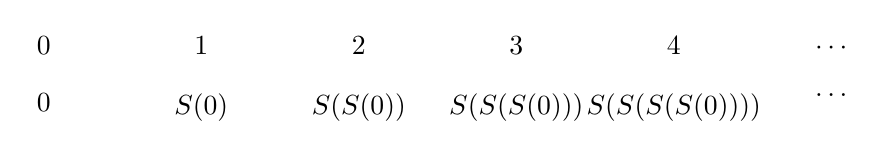
\begin{tikzpicture}
		\coordinate (number0) at (0,0);
		\coordinate (number1) at (2cm,0);
		\coordinate (number2) at (4cm,0);
		\coordinate (number3) at (6cm,0);
		\coordinate (number4) at (8cm,0);
		\coordinate (etc) at (10cm,0);

		\node[label={[black]above:$0$},label={[black]below:$0$}] at (number0) {};
		\node[label={[black]above:$1$},label={[black]below:$S(0)$}] at (number1) {};
		\node[label={[black]above:$2$},label={[black]below:$S(S(0))$}] at (number2) {};
		\node[label={[black]above:$3$},label={[black]below:$S(S(S(0)))$}] at (number3) {};
		\node[label={[black]above:$4$},label={[black]below:$S(S(S(S(0))))$}] at (number4) {};
		\node[label={[black]above:$\cdots$},label={[black]below:$\ldots$}] at (etc) {};
	\end{tikzpicture}
	\caption{Năm phần tử đầu tiên của tập hợp số tự nhiên theo hệ tiên đề Peano.}\label{fig:first-five-natural-numbers}
\end{figure}

Ý niệm và kí hiệu cho các số tự nhiên được xuất hiện trước hệ tiên đề của Peano hàng nghìn năm. Các kí hiệu (các số) $1, 2, 3,\ldots$ lần lượt chính là $S(0), S(S(0)), S(S(S(0))),\ldots$

Chúng tôi muốn nhấn mạnh một lần nữa: trong hai mục tiếp theo, chúng ta sẽ áp dụng liên tục phương pháp quy nạp toán học.

\subsection*{$\dagger$ Các phép toán số học trên tập hợp số tự nhiên}

Bạn đọc không cần quá chú ý tới kĩ thuật chứng minh trong mục này. Tuy nhiên, chúng tôi cung cấp chứng minh chậm rãi và chi tiết cho mục đích tham khảo. Luận cho cùng, mọi thứ được xây dựng từ các số tự nhiên.

Hai phép toán cơ bản với số tự nhiên là phép cộng và phép nhân. Trong mục này, chúng ta sẽ định nghĩa hai phép toán cộng và nhân trên tập hợp số tự nhiên theo hệ tiên đề Peano, sau đó chứng minh các tính chất cơ bản của chúng.

Phép cộng hai số tự nhiên được định nghĩa bằng đệ quy như sau.

\begin{definition}[Phép cộng]
	Cho $x$ và $y$ là hai số tự nhiên. Phép cộng hai số tự nhiên là một phép toán hai ngôi trên $\mathbb{N}$, kí hiệu là $+$. Phép cộng hai số tự nhiên $a$ và $b$ cho ra kết quả là một số tự nhiên, được kí hiệu là $a + b$, được gọi là \textbf{tổng} của $a$ và $b$. Chúng ta định nghĩa
	\[
		x + 0 = x\qquad\text{và}\qquad x + S(y) = S(x + y).
	\]
\end{definition}

Nhằm minh họa cho định nghĩa này, chúng ta làm một vài phép cộng.
\begin{example}
	Cho số tự nhiên $x$.
	\begin{align*}
		 & x + 0 = x,                                      \\
		 & x + S(0) = S(x + 0) = S(x),                     \\
		 & x + S(1) = x + S(S(0)) = S(x + S(0)) = S(S(x)).
	\end{align*}
\end{example}

Chúng ta sử dụng nguyên lý quy nạp toán học để chứng minh hai tính chất kết hợp và tính chất giao hoán của phép cộng hai số tự nhiên.
\begin{theorem}\label{theorem:property-of-natural-numbers-addition}
	Trên tập hợp số tự nhiên
	\begin{enumerate}[label={(\roman*)}]
		\item Phép cộng có tính chất kết hợp. Tức là, với mọi số tự nhiên $x, y, z$, chúng ta có $(x + y) + z = x + (y + z)$. Bằng kí hiệu logic hình thức, chúng ta viết
		      \[
			      \forall x\forall y\forall z \left( (x + y) + z = x + (y + z) \right).
		      \]
		\item Với mọi số tự nhiên $x$, có $0 + x = x$.
		\item Phép cộng có tính chất giao hoán.  Tức là, với mọi số tự nhiên $x, y$, chúng ta có $x + y = y + x$. Bằng kí hiệu logic hình thức, chúng ta viết
		      \[
			      \forall x\forall y \left( x + y = y + x \right).
		      \]
	\end{enumerate}
\end{theorem}

\begin{proof}
	\begin{enumerate}[label={(\roman*)}]
		\item Nếu $z = 0$ thì $(x + y) + z = x + y = x + (y + 0) = x + (y + z)$.

		      Giả sử với số tự nhiên $z = n$, $(x + y) + n = x + (y + n)$. Chúng ta sẽ chứng minh $(x + y) + S(n) = x + (y + S(n))$.
		      \begin{align*}
			      (x + y) + S(n) & = S((x + y) + n)  & \text{(theo định nghĩa phép cộng trên $\mathbb{N}$)} \\
			                     & = S(x + (y + n))  & \text{(theo giả thiết quy nạp)}                      \\
			                     & = x + S(y + n)    & \text{(theo định nghĩa phép cộng trên $\mathbb{N}$)} \\
			                     & = x + (y + S(n)). & \text{(theo định nghĩa phép cộng trên $\mathbb{N}$)}
		      \end{align*}

		      Vậy theo nguyên lý quy nạp toán học, $(x + y) + z = x + (y + z)$ với mọi số tự nhiên $x, y, z$.
		\item Khi $x = 0$, $0 + 0 = 0$, theo định nghĩa phép cộng trên tập hợp số tự nhiên.

		      Giả sử với số tự nhiên $x = n$, $0 + n = n$. Khi đó
		      \begin{align*}
			      0 + S(n) & = S(0 + n) & \text{(theo định nghĩa phép cộng trên $\mathbb{N}$)} \\
			               & = S(n).    & \text{(theo giả thiết quy nạp)}
		      \end{align*}

		      Theo nguyên lý quy nạp toán học, $0 + x = x$ với mọi số tự nhiên $x$.
		\item Khi $y = 0$ thì $x + 0 = x = 0 + x$, theo định nghĩa phép cộng hai số tự nhiên và phần (ii).

		      Chúng tôi gặp khó khăn khi cố gắng chứng minh tính chất giao hoán của phép cộng hai số tự nhiên bằng \textit{một lần} quy nạp. Trước hết, chúng ta chứng minh mệnh đề sau: $x + S(0) = S(0) + x$ với mọi số tự nhiên $x$.

		      Khi $x = 0$, theo định nghĩa phép cộng hai số tự nhiên, $0 + S(0) = S(0 + 0) = S(0) = S(0) + 0$.

		      Giả sử với số tự nhiên $x = n$, có $n + S(0) = S(0) + n$. Khi đó
		      \begin{align*}
			      S(0) + S(n) & = S(S(0) + n)  & \text{(theo định nghĩa phép cộng trên $\mathbb{N}$)} \\
			                  & = S(n + S(0))  & \text{(theo giả thiết quy nạp)}                      \\
			                  & = S(S(n))      & \text{(theo định nghĩa phép cộng trên $\mathbb{N}$)} \\
			                  & = S(S(n) + 0)  & \text{(theo định nghĩa phép cộng trên $\mathbb{N}$)} \\
			                  & = S(n) + S(0). & \text{(theo định nghĩa phép cộng trên $\mathbb{N}$)}
		      \end{align*}

		      Theo nguyên lý quy nạp toán học, $x + S(0) = S(0) + x$ với mọi số tự nhiên $x$.

		      Chúng ta thực hiện chứng minh bằng quy nạp một lần nữa cho mệnh đề $x + y = y + x$ với mọi số tự nhiên $x, y$.

		      Khi $y = 0$ và khi $y = S(0)$, chúng ta lần lượt có $x + 0 = x = 0 + x$ (theo phần (ii)) và $x + S(0) = S(0) + x$ (theo mệnh đề vừa chứng minh).

		      Giả sử với số tự nhiên $y = n$, $x + n = n + x$. Khi đó
		      \begin{align*}
			      x + S(n) & = S(x + n)       & \text{(theo định nghĩa phép cộng trên $\mathbb{N}$)} \\
			               & = S(n + x)       & \text{(theo giả thiết quy nạp)}                      \\
			               & = S((n + x) + 0) & \text{(theo định nghĩa phép cộng trên $\mathbb{N}$)} \\
			               & = (n + x) + S(0) & \text{(theo định nghĩa phép cộng trên $\mathbb{N}$)} \\
			               & = S(0) + (n + x) & \text{(theo mệnh đề vừa chứng minh)}                 \\
			               & = (S(0) + n) + x & \text{(theo phần (i))}                               \\
			               & = (n + S(0)) + x & \text{(theo mệnh đề vừa chứng minh)}                 \\
			               & = S(n) + x.      & \text{(theo định nghĩa phép cộng trên $\mathbb{N}$)}
		      \end{align*}

		      Theo nguyên lý quy nạp toán học, $x + y = y + x$ với mọi số tự nhiên $x, y$.
	\end{enumerate}
\end{proof}

Sư góp mặt của số $0$ trong phép toán cộng các số tự nhiên dẫn tới những trường hợp  đặc biệt.
\begin{theorem}\label{theorem:addition-and-zero}
	\begin{enumerate}[label={(\roman*)}]
		\item Với mọi số tự nhiên $x$, $x + y = x$ kéo theo $y = 0$.
		\item Hai số tự nhiên $a$ và $b$ thỏa mãn $a + b = 0$ khi và chỉ khi $a = b = 0$.
		\item Hai số tự nhiên $a$ và $b$ thỏa mãn $a + b = 1$ khi và chỉ khi $a = 0, b = 1$ hoặc $a = 1, b = 0$.
	\end{enumerate}
\end{theorem}

\begin{proof}
	\begin{enumerate}[label={(\roman*)}]
		\item Với mọi số tự nhiên $x$, $x + y = x$ kéo theo $y = 0$.

		      Khi $x = 0$ thì $y = 0 + y = 0$. Giả sử với $x = n$, chúng ta có ``$n + y = n$ kéo theo $y = 0$''. Khi đó, nếu $S(n) + y = S(n)$ thì
		      \begin{align*}
			      S(n + y) & = S(y + n) & \text{(theo tính chất giao hoán của phép cộng trên $\mathbb{N}$)} \\
			               & = y + S(n) & \text{(theo định nghĩa phép cộng trên $\mathbb{N}$)}              \\
			               & = S(n) + y & \text{(theo tính chất giao hoán của phép cộng trên $\mathbb{N}$)} \\
			               & = S(n).
		      \end{align*}

		      Từ đẳng thức $S(n + y) = S(n)$, theo tiên đề 7, chúng ta có $n + y = n$. Theo giả thiết quy nạp, $y = 0$. Do đó $S(n) + y = S(n)$ kéo theo $y = 0$. Như vậy, theo nguyên lý quy nạp, với mọi số tự nhiên $x$, $x + y = x$ kéo theo $y = 0$.

		      Vậy khi hai số tự nhiên $x, y$ thỏa mãn $x + y = x$ thì $y = 0$.
		\item ($\Rightarrow$) $a = b = 0$.

		      Theo định nghĩa phép cộng trên tập hợp số tự nhiên, $a + b = 0 + 0 = 0$.

		      ($\Leftarrow$) $a + b = 0$.

		      Giả sử phản chứng rằng $a\ne 0$. Khi đó tồn tại số tự nhiên $c$ sao cho $S(c) = a$. Theo định nghĩa phép cộng hai số tự nhiên và tính chất giao hoán của phép cộng hai số tự nhiên, chúng ta có $0 = b + a = b + S(c) = S(b + c)$. Điều này mâu thuẫn với tiên đề 8. Do đó $a = 0$.

		      Tương tự, cũng bằng phương pháp phản chứng, chúng ta chỉ ra được $b = 0$.

		      Vậy hai số tự nhiên $a, b$ thỏa mãn $a + b = 0$ khi và chỉ khi $a = b = 0$.
		\item ($\Rightarrow$) $a = 1, b = 0$ hoặc $a = 0, b = 1$.

		      Vì với mọi số tự nhiên $x$, có $x + 0 = 0 + x = x$ nên trong cả hai trường hợp $a = 1, b = 0$ hay $a = 0, b = 1$, chúng ta đều có $a + b = 1$.

		      ($\Leftarrow$) $a + b = 1$.

		      $a$ và $b$ không thể đồng thời bằng $0$ (vì khi đó $a + b = 0$, điều này mâu thuẫn với việc $a + b = 1$). Do đó ít nhất một trong hai số tự nhiên $a$ và $b$ khác $0$.

		      Nếu $b\ne 0$ thì theo Định lý~\ref{theorem:successor}, tồn tại số tự nhiên $n$ sao cho $b = S(n)$. Theo định nghĩa phép cộng hai số tự nhiên, $S(0) = 1 = a + b = a + S(n) = S(a + n)$. Theo tiên đề 7, chúng ta có $a + n = 0$. Theo phần (ii), $a = n = 0$, kéo theo $b = 1$.

		      Nếu $a\ne 0$ thì theo Định lý~\ref{theorem:successor}, tồn tại số tự nhiên $m$ sao cho $a = S(m)$. Theo tính chất giao hoán của phép cộng số tự nhiên và định nghĩa phép cộng hai số tự nhiên, $S(0) = 1 = a + b = b + a = b + S(m) = S(b + m)$. Theo tiên đề 7, chúng ta có $b + m = 0$. Theo phần (ii), $b = m = 0$, kéo theo $a = 1$.

		      Vậy hai số tự nhiên $a$ và $b$ thỏa mãn $a + b = 1$ khi và chỉ khi $a = 0, b = 1$ hoặc $a = 1, b = 0$.
	\end{enumerate}
\end{proof}

Phép nhân cũng được định nghĩa bằng đệ quy.
\begin{definition}[Phép nhân]
	Cho $x$ và $y$ là hai số tự nhiên. Phép nhân hai số tự nhiên là một phép toán hai ngôi trên $\mathbb{N}$, kí hiệu là $\cdot$. Phép nhân hai số tự nhiên $a$ và $b$ cho ra kết quả là một số tự nhiên, được kí hiệu là $a\cdot b$, được gọi là \textbf{tích} của $a$ và $b$. Chúng ta định nghĩa
	\[
		x\cdot 0 = 0\qquad\text{và}\qquad x\cdot S(y) = x + (x\cdot y).
	\]
\end{definition}

Tương tự, chúng ta làm một vài phép nhân với định nghĩa này.

\begin{example}
	Cho số tự nhiên $x$.
	\begin{align*}
		 & x \cdot 0 = 0,                                                                 \\
		 & x \cdot 1 = x\cdot S(0) = x + (x\cdot 0) = x + 0 = x,                          \\
		 & x \cdot 2 = x\cdot S(S(0)) = x + (x\cdot S(0)) = x + (x + (x\cdot 0)) = x + x.
	\end{align*}
\end{example}

Chúng ta nhắc lại và chứng minh các tính chất sau của phép nhân hai số tự nhiên.

\begin{theorem}\label{theorem:property-of-natural-numbers-multiplication}
	Trên tập hợp số tự nhiên
	\begin{enumerate}[label={(\roman*)}]
		\item Phép nhân có tính chất phân phối (từ bên phải) với phép cộng. Nói cách khác, với mọi số tự nhiên $x, y, z$, chúng ta có $(x + y)\cdot z = (x\cdot z) + (y\cdot z)$.
		\item Phép nhân có tính chất kết hợp. Nói cách khác, với mọi số tự nhiên $x, y, z$, chúng ta có $(x \cdot y) \cdot z = x \cdot (y \cdot z)$. Bằng kí hiệu logic hình thức, chúng ta viết
		      \[
			      \forall x\forall y\forall z \left( (x \cdot y) \cdot z = x \cdot (y \cdot z) \right).
		      \]
		\item Với mọi só tự nhiên $x$, $0\cdot x = 0$.
		\item Với mọi số tự nhiên $x$, $x\cdot S(0) = S(0) \cdot x = x$.
		\item Phép nhân có tính chất giao hoán. Nói cách khác, với mọi số tự nhiên $x, y$, chúng ta có $x \cdot y = y \cdot x$. Bằng kí hiệu logic hình thức, chúng ta viết
		      \[
			      \forall x\forall y \left( x \cdot y = y \cdot x \right).
		      \]
	\end{enumerate}
\end{theorem}

\begin{proof}
	\begin{enumerate}[label={(\roman*)}]
		\item Nếu $z = 0$ thì theo định nghĩa phép nhân và phép cộng hai số tự nhiên
		      \begin{align*}
			      (x + y)\cdot z & = (x + y)\cdot 0 = 0 = 0 + 0 = (x\cdot 0) + (y\cdot 0) = (x\cdot z) + (y\cdot z).
		      \end{align*}

		      Giả sử với $z = n$, có $(x + y)\cdot n = (x\cdot n) + (y\cdot n)$. Khi đó
		      \begin{align*}
			      (x + y)\cdot S(n) & = (x + y) + (x + y)\cdot n            & \text{(theo định nghĩa phép nhân trên $\mathbb{N}$)}              \\
			                        & = (x + y) + ((x\cdot n) + (y\cdot n)) & \text{(theo giả thiết quy nạp)}                                   \\
			                        & = ((x + y) + (x\cdot n)) + (y\cdot n) & \text{(theo tính chất kết hợp của phép cộng trên $\mathbb{N}$)}   \\
			                        & = (x + (y + (x\cdot n))) + (y\cdot n) & \text{(theo tính chất kết hợp của phép cộng trên $\mathbb{N}$)}   \\
			                        & = (x + ((x\cdot n) + y)) + (y\cdot n) & \text{(theo tính chất giao hoán của phép cộng trên $\mathbb{N}$)} \\
			                        & = ((x + (x\cdot n)) + y) + (y\cdot n) & \text{(theo tính chất kết hợp của phép cộng trên $\mathbb{N}$)}   \\
			                        & = (x + (x\cdot n)) + (y + (y\cdot n)) & \text{(theo tính chất kết hợp của phép cộng trên $\mathbb{N}$)}   \\
			                        & = (x\cdot S(n)) + (y\cdot S(n)).      & \text{(theo định nghĩa của phép nhân trên $\mathbb{N}$)}
		      \end{align*}

		      Theo nguyên lý quy nạp toán học, $(x + y)\cdot z = (x\cdot z) + (y\cdot z)$ với mọi số tự nhiên $x, y, z$.
		\item Nếu $z = 0$ thì theo định nghĩa phép nhân hai số tự nhiên, $(x\cdot y)\cdot z = 0 = x\cdot 0 = x\cdot (y\cdot 0) = x\cdot (y\cdot z)$.

		      Giả sử với số tự nhiên $z = n$, có $(x\cdot y)\cdot n = x\cdot (y\cdot n)$. Khi đó
		      \begin{align*}
			      (x\cdot y)\cdot S(n) & = (x\cdot y) + ((x\cdot y)\cdot n) & \text{(theo định nghĩa phép nhân trên $\mathbb{N}$)}            \\
			                           & = (x\cdot y) + (x\cdot (y\cdot n)) & \text{(theo tính chất kết hợp của phép nhân trên $\mathbb{N}$)} \\
			                           & = x\cdot (y + (y\cdot n))          & \text{(theo phần (i))}                                          \\
			                           & = x\cdot (y\cdot S(n)).            & \text{(theo định nghĩa phép nhân trên $\mathbb{N}$)}
		      \end{align*}

		      Theo nguyên lý quy nạp toán học, $(x\cdot y)\cdot z = x\cdot (y\cdot z)$ với mọi số tự nhiên $x, y, z$.
		\item Khi $x = 0$, chúng ta có $0\cdot x = 0\cdot 0 = 0$, theo định nghĩa phép nhân trên tập số tự nhiên.

		      Giả sử với $x = n$, chúng ta có $0\cdot n = 0$. Khi đó
		      \begin{align*}
			      0\cdot S(n) & = 0 + (0\cdot n) & \text{(theo định nghĩa phép nhân trên $\mathbb{N}$)} \\
			                  & = 0 + 0          & \text{(theo giả thiết quy nạp)}                      \\
			                  & = 0.             & \text{(theo định nghĩa phép cộng trên $\mathbb{N}$)}
		      \end{align*}

		      Theo nguyên lý quy nạp toán học, $0\cdot x = 0$ với mọi số tự nhiên $x$.
		\item Theo định nghĩa phép nhân và phép cộng hai số tự nhiên, $x\cdot S(0) = x + (x\cdot 0) = x + 0 = x$.

		      Chúng ta cần chứng minh $S(0)\cdot x = x$ với mọi số tự nhiên $x$. Khi $x = 0$, chúng ta có $S(0)\cdot 0 = 0$, theo định nghĩa của phép nhân hai số tự nhiên.

		      Giả sử với số tự nhiên $x = n$, chúng ta có $S(0)\cdot n = n$. Khi đó
		      \begin{align*}
			      S(0)\cdot S(n) & = S(0) + (S(0)\cdot n) & \text{(theo định nghĩa của phép nhân trên $\mathbb{N}$)}          \\
			                     & = S(0) + n             & \text{(theo giả thiết quy nạp)}                                   \\
			                     & = n + S(0)             & \text{(theo tính chất giao hoán của phép cộng trên $\mathbb{N}$)} \\
			                     & = S(n).                & \text{(theo định nghĩa của phép cộng trên $\mathbb{N}$)}
		      \end{align*}

		      Theo nguyên lý quy nạp toán học, $x\cdot S(0) = S(0)\cdot x = x$ với mọi số tự nhiên $x$.
		\item Khi $y = 0$, theo định nghĩa phép nhân trên tập hợp số tự nhiên và phần (iii), chúng ta có $x\cdot 0 = 0\cdot x = 0$.

		      Giả sử với số tự nhiên $y = n$, chúng ta có $x\cdot n = n\cdot x$. Khi đó
		      \begin{align*}
			      x\cdot S(n) & = x + (x\cdot n)             & \text{(định nghĩa phép nhân trên $\mathbb{N}$)}                   \\
			                  & = x + (n\cdot x)             & \text{(theo giả thiết quy nạp)}                                   \\
			                  & = (S(0)\cdot x) + (n\cdot x) & \text{(theo phần (iv))}                                           \\
			                  & = (S(0) + n)\cdot x          & \text{(theo phần (i))}                                            \\
			                  & = (n + S(0))\cdot x          & \text{(theo tính chất giao hoán của phép cộng trên $\mathbb{N}$)} \\
			                  & = S(n)\cdot x.               & \text{(theo định nghĩa phép cộng trên $\mathbb{N}$)}
		      \end{align*}

		      Theo nguyên lý quy nạp toán học, $x\cdot y = y\cdot x$ với mọi số tự nhiên $x, y$.
	\end{enumerate}
\end{proof}

Với những tính chất đã chứng minh của phép cộng và phép nhân hai số tự nhiên, chúng ta rút ra hệ quả sau.

\begin{corollary}
	Trên tập hợp số tự nhiên, phép nhân có tính chất phân phối với phép cộng (từ cả hai phía). Bằng kí hiệu, điều này nghĩa là với mọi số tự nhiên $x, y, z$, chúng ta có
	\[
		\begin{split}
			(x + y)\cdot z = (x\cdot z) + (y\cdot z), \\
			z\cdot (x + y) = (z\cdot x) + (z\cdot y).
		\end{split}
	\]
\end{corollary}

Tương tự với phép cộng, phép nhân với $0$ cũng là một trường hợp đặc biệt.
\begin{theorem}\label{theorem:zero-one-and-natural-numbers-multiplication}
	Cho hai số tự nhiên $x$ và $y$, khi đó
	\begin{enumerate}[label={(\roman*)}]
		\item $x\cdot y = 0$ khi và chỉ khi $x = 0$ hoặc $y = 0$.
		\item $x\cdot y = 1$ khi và chỉ khi $x = y = 1$.
	\end{enumerate}
\end{theorem}

\begin{proof}
	\begin{enumerate}[label={(\roman*)}]
		\item ($\Rightarrow$) $x = 0$ hoặc $y = 0$.

		      Theo định nghĩa phép nhân hai số tự nhiên và phần (iii) của Định lý~\ref{theorem:property-of-natural-numbers-multiplication}, chúng ta suy ra $x\cdot y = 0$.

		      ($\Leftarrow$) $x\cdot y = 0$.

		      Nếu $x\ne 0$ thì theo Định lý~\ref{theorem:successor}, tồn tại số tự nhiên $a$ sao cho $S(a) = x$.
		      \begin{align*}
			      0 & = x\cdot y = S(a)\cdot y                                                                \\
			        & = y\cdot S(a)            & \text{(tính chất giao hoán của phép nhân trên $\mathbb{N}$)} \\
			        & = y + y\cdot a           & \text{(theo định nghĩa của phép nhân trên $\mathbb{N}$)}
		      \end{align*}

		      Theo phần (ii) của Định lý~\ref{theorem:addition-and-zero}, $y = 0$.

		      Nếu $y\ne 0$ thì theo Định lý~\ref{theorem:successor}, tồn tại số tự nhiên $b$ sao cho $S(b) = y$.
		      \begin{align*}
			      0 & = x\cdot y = x\cdot S(b)                                                            \\
			        & = x + x\cdot b           & \text{(theo định nghĩa của phép nhân trên $\mathbb{N}$)}
		      \end{align*}

		      Theo phần (ii) của Định lý~\ref{theorem:addition-and-zero}, $x = 0$.

		      Do đó $x\cdot y = 0$ kéo theo $x = 0$ hoặc $y = 0$.

		      Vậy với hai số tự nhiên $x$ và $y$, $x\cdot y = 0$ khi và chỉ khi $x = 0$ hoặc $y = 0$.
		\item ($\Rightarrow$) $x = 1$ và $y = 1$.

		      Theo Định lý~\ref{theorem:property-of-natural-numbers-multiplication}, $1\cdot 1 = S(0)\cdot S(0) = S(0) = 1$.

		      ($\Leftarrow$) $x\cdot y = 1$.

		      Theo phần (i), $x\ne 0$ và $y\ne 0$. Theo Định lý~\ref{theorem:successor}, tồn tại hai số tự nhiên $a$ và $b$ sao cho $S(a) = x$ và $S(b) = y$. Theo định nghĩa phép cộng, phép nhân hai số tự nhiên, và tính chất giao hoán của phép cộng hai số tự nhiên
		      \begin{align*}
			      S(0) & = 1 = x\cdot y                       \\
			           & = x\cdot S(b) = x + (x\cdot b)       \\
			           & = (x\cdot b) + x = (x\cdot b) + S(a) \\
			           & = S((x\cdot b) + a).
		      \end{align*}

		      Theo tiên đề 7, $(x\cdot b) + a = 0$. Theo Định lý~\ref{theorem:addition-and-zero}, $x\cdot b = a = 0$. Mà $x\ne 0$ nên theo phần (i), chúng ta có $b = 0$. Vì $a = b = 0$ nên $x = y = S(0) = 1$.

		      Vậy với hai số tự nhiên $x$ và $y$, $x\cdot y = 1$ khi và chỉ khi $x = 1$ hoặc $y = 1$.
	\end{enumerate}
\end{proof}

Chúng ta khép lại nội dung về phép cộng và phép nhân trên tập số tự nhiên bằng một lưu ý. Thói quen học tập, tính toán, và cả các chứng minh trong mục này có thể gây ra một ấn tượng \textit{không chính xác} rằng tính chất kết hợp và tính chất giao hoán luôn song hành. Thực tế, khi học và làm toán, chúng ta sẽ bắt gặp những phép toán trên những tập hợp nhất định mà \textit{không có tính chất kết hợp lẫn giao hoán}, hoặc \textit{có tính chất giao hoán nhưng không có tính chất kết hợp}, hoặc \textit{có tính chất kết hợp mà không có tính chất giao hoán} (chẳng hạn như phép toán hợp thành hai ánh xạ).

\subsection*{$\dagger$ Quan hệ thứ tự trên tập hợp số tự nhiên}

Số tự nhiên đã trở nên quá quen thuộc với chúng ta, đến nỗi việc nói rằng số này bé hơn số kia được coi là hiển nhiên. Tuy nhiên, để học và làm toán, chúng ta vẫn cần những định nghĩa hình thức tương thích với hệ tiên đề và những định lý mà chúng ta sử dụng.

\begin{definition}[Quan hệ thứ tự trên tập hợp số tự nhiên]
	Số tự nhiên $x$ được gọi là nhỏ hơn hoặc bằng số tự nhiên $y$ nếu và chỉ nếu tồn tại số tự nhiên $z$ sao cho $x + z = y$. Khi đó, chúng ta kí hiệu $x\leq y$. Nếu $x\leq y$ và $x\ne y$ thì chúng ta nói $x$ nhỏ hơn $y$ và kí hiệu $x < y$.

	Nói riêng, nếu $x + 1 = y$ hoặc $y + 1 = x$ thì chúng ta nói $x$ và $y$ là hai số tự nhiên liên tiếp.
\end{definition}

Các phát biểu $x < y$, $x\leq y$, $x > y$, $x\geq y$ được gọi là các bất đẳng thức.

Với định nghĩa trên, chúng ta vẫn phải kiểm tra quan hệ nhỏ hơn hoặc bằng trên tập hợp số tự nhiên có thỏa mãn ba tính chất của quan hệ thứ tự hay không. Việc chứng minh tính chất phản đối xứng tỏ ra khó khăn hơn cả.

\begin{proposition}
	Chứng minh rằng
	\begin{enumerate}[label={(\roman*)}]
		\item Quan hệ $\leq$ trên tập hợp số tự nhiên thỏa mãn tính chất phản xạ và bắc cầu.
		\item Với mọi số tự nhiên $x$, có $x\ne S(x)$.
		\item Quan hệ $\leq$ trên tập hợp số tự nhiên thỏa mãn tính chất phản đối xứng.
		\item Quan hệ $\leq$ trên tập hợp số tự nhiên là một quan hệ thứ tự toàn phần.
	\end{enumerate}
\end{proposition}

\begin{proof}
	\begin{enumerate}[label={(\roman*)}]
		\item Với mọi số tự nhiên, chúng ta có $x + 0 = x$. Do đó $x\leq x$. Như vậy quan hệ $\leq$ trên tập hợp số tự nhiên có tính chất phản xạ.

		      Nếu ba số tự nhiên $x, y, z$ thỏa mãn $x\leq y$ và $y\leq z$ thì theo định nghĩa của $\leq$, tồn tại các số tự nhiên $m$ và $n$ sao cho $x + m = y$ và $y + n = z$. Khi đó
		      \begin{align*}
			      z & = y + n       \\
			        & = (x + m) + n \\
			        & = x + (m + n)
		      \end{align*}

		      Theo định nghĩa của $\leq$, chúng ta suy ra $x\leq z$. Như vậy quan hệ $\leq$ trên tập hợp số tự nhiên có tính chất bắc cầu.
		\item Khi $x = 0$, $0\ne S(0)$ theo tiên đề 8.

		      Giả sử với số tự nhiên $x = n$, có $n\ne S(n)$. Theo giả thiết quy nạp và tiên đề 7, $S(n)\ne S(S(n))$.

		      Vậy theo nguyên lý quy nạp toán học, $x\ne S(x)$ với mọi số tự nhiên $x$.
		\item Nếu hai số tự nhiên $x$ và $y$ thỏa mãn $x\leq y$ và $y\leq x$ thì theo định nghĩa quan hệ $\leq$ trên tập hợp số tự nhiên, tồn tại hai số tự nhiên $a$ và $b$ sao cho $x + a = y$ và $y + b = x$. Khi đó
		      \begin{align*}
			      x & = y + b                                                                         \\
			        & = (x + a) + b                                                                   \\
			        & = x + (a + b) & \text{(theo tính chất kết hợp của phép cộng trên $\mathbb{N}$)}
		      \end{align*}

		      Theo phần (i) và (ii) của Định lý~\ref{theorem:addition-and-zero}, chúng ta kết luận $a = b = 0$, dẫn tới $x = y$. Như vậy, quan hệ $\leq$ trên tập hợp số tự nhiên có tính chất phản đối xứng.
		\item Phần (i) và (iii) khẳng định rằng quan hệ $\leq$ trên tập hợp số tự nhiên là một quan hệ thứ tự.

		      Để chứng minh quan hệ $\leq$ trên tập hợp số tự nhiên là quan hệ thứ tự toàn phần, chúng ta chứng minh: Với mọi số tự nhiên $x, y$, có $x\leq y$ hoặc $y\leq x$.

		      Đầu tiên, với mọi số tự nhiên $x$, có $0\leq x$ hoặc $x\leq 0$. Giả sử với số tự nhiên $y = n$, với mọi số tự nhiên $x$, có $n\leq x$ hoặc $x\leq n$. Sử dụng giả thiết quy nạp, chúng ta xem xét hai trường hợp sau.

		      Trường hợp $x\leq n$. Theo định nghĩa phép cộng hai số tự nhiên, $n + S(0) = S(n)$ nên $n\leq S(n)$ theo định nghĩa quan hệ $\leq$ trên tập hợp số tự nhiên. Từ tính chất bắc cầu của quan hệ $\leq$ trên tập hợp số tự nhiên, chúng ta suy ra $x\leq S(n)$.

		      Trường hợp $n\leq x$. Theo định nghĩa quan hệ thứ tự trên tập hợp số tự nhiên, tồn tại số tự nhiên $a$ sao cho $n + a = x$. Nếu $x = n$ thì $x\leq S(n)$ vì $n\leq S(n)$ (rút ra từ phần chứng minh của trường hợp trên). Còn nếu $n < x$ thì $a$ khác không (theo Định lý~\ref{theorem:addition-and-zero}). Theo Định lý~\ref{theorem:successor}, vì $a$ khác không nên tồn tại số tự nhiên $b$ sao cho $a = S(b)$. Theo định nghĩa phép cộng hai số tự nhiên, $x = n + a = n + S(b) = S(n + b)$. Bên cạnh đó, $S(n) + b = b + S(n) = S(b + n) = S(n + b) = x$, nên theo định nghĩa quan hệ $\leq$ trên tập hợp số tự nhiên, chúng ta có $S(n)\leq x$.

		      Tóm lại, từ cả hai trường hợp, chúng ta kết luận: với mọi số tự nhiên $x$, $x\leq S(n)$ hoặc $S(n)\leq x$. Theo nguyên lý quy nạp, với mọi cặp số tự nhiên $x$ và $y$, có $x\leq y$ hoặc $y\leq x$.

		      Vậy quan hệ $\leq$ trên tập hợp số tự nhiên là một quan hệ thứ tự toàn phần.\qedhere
	\end{enumerate}
\end{proof}

Sự liên hệ giữa quan hệ $\leq$ và hai phép toán cộng và nhân trên tập hợp số tự nhiên được trình bày trong định lý sau.
\begin{theorem}\label{theorem:natural-numbers-order}
	Với mọi số tự nhiên $x, y, z$
	\begin{enumerate}[label={(\roman*)}]
		\item $x\leq y$ khi và chỉ khi $x + z\leq y + z$.
		\item $x\leq y$ kéo theo $x\cdot z\leq y\cdot z$.
	\end{enumerate}
\end{theorem}

\noindent Chúng ta sử dụng mệnh đề sau để chứng minh định lý trên.

\begin{proposition}\label{proposition:addition-cancellation}
	Với mọi số tự nhiên $x, y, z$, nếu $x + z = y + z$ thì $x = y$.
\end{proposition}

\begin{proof}
	Với mọi số tự nhiên $x, y$:

	Khi $z = 0$, nếu $x + 0 = y + 0$ thì $x = y$ (theo định nghĩa phép cộng hai số tự nhiên).

	Giả sử với số tự nhiên $z = n$, $x + n = y + n$ kéo theo $x = y$. Khi đó chúng ta chứng minh rằng $x + S(n) = y + S(n)$ kéo theo $x = y$. Nếu $x + S(n) = y + S(n)$ thì theo định nghĩa phép cộng hai số tự nhiên, chúng ta có $S(x + n) = S(y + n)$. Theo tiên đề 7 thì $x + n = y + n$. Theo giả thiết quy nạp, $x = y$. Do đó $x + S(n) = y + S(n)$ kéo theo $x = y$.

	Theo nguyên lý quy nạp toán học, với mọi số tự nhiên $x, y, z$, nếu $x + z = y + z$ thì $x = y$.
\end{proof}

\begin{proof}[Chứng minh Định lý~\ref{theorem:natural-numbers-order}]
	\begin{enumerate}[label={(\roman*)}]
		\item ($\Rightarrow$) $x\leq y$.

		      Theo định nghĩa quan hệ $\leq$ trên tập hợp số tự nhiên, tồn tại số tự nhiên $a$ sao cho $x + a = y$. Khi đó
		      \begin{align*}
			      (x + z) + a & = x + (z + a) & \text{(theo tính chất kết hợp của phép cộng trên $\mathbb{N}$)}   \\
			                  & = x + (a + z) & \text{(theo tính chất giao hoán của phép cộng trên $\mathbb{N}$)} \\
			                  & = (x + a) + z & \text{(theo tính chất kết hợp của phép cộng trên $\mathbb{N}$)}   \\
			                  & = y + z.
		      \end{align*}

		      Theo định nghĩa quan hệ $\leq$ trên tập hợp số tự nhiên, chúng ta suy ra $x + z\leq y + z$.

		      ($\Leftarrow$) $x + z\leq y + z$.

		      Theo định nghĩa quan hệ $\leq$ trên tập hợp số tự nhiên, tồn tại số tự nhiên $a$ sao cho $(x + z) + a = y + z$. Bên cạnh đó
		      \begin{align*}
			      (x + z) + a & = x + (z + a)  & \text{(theo tính chất kết hợp của phép cộng trên $\mathbb{N}$)}   \\
			                  & = x + (a + z)  & \text{(theo tính chất giao hoán của phép cộng trên $\mathbb{N}$)} \\
			                  & = (x + a) + z. & \text{(theo tính chất kết hợp của phép cộng trên $\mathbb{N}$)}
		      \end{align*}

		      Từ hai đẳng thức $(x + z) + a = y + z$ và $(x + z) + a = (x + a) + z$, chúng ta suy ra $(x + a) + z = y + z$. Theo Mệnh đề~\ref{proposition:addition-cancellation}, chúng ta suy ra $x + a = y$. Theo định nghĩa quan hệ $\leq$ trên tập hợp số tự nhiên, $x\leq y$.

		      Vậy với mọi số tự nhiên $x, y, z$, $x\leq y$ khi và chỉ khi $x + z \leq y + z$.
		\item Với mọi số tự nhiên $x, y$:

		      Khi $z = 0$, nếu $x\leq y$ thì $x\cdot 0\leq y\cdot 0$, vì $x\cdot 0 = y\cdot 0 = 0$.

		      Giả sử với số tự nhiên $z = n$, chúng ta có $x\leq y$ kéo theo $x\cdot n\leq y\cdot n$. Khi đó, theo định nghĩa phép nhân hai số tự nhiên
		      \[
			      \begin{split}
				      x\cdot S(n) = x + (x\cdot n) \\
				      y\cdot S(n) = y + (y\cdot n)
			      \end{split}
		      \]

		      Theo giả thiết quy nạp, tính chất giao hoán của phép cộng hai số tự nhiên, phần (i), tính chất bắc cầu của quan hệ $\leq$ trên tập hợp số tự nhiên, và định nghĩa phép nhân hai số tự nhiên, chúng ta suy ra
		      \begin{align*}
			      x\cdot S(n) & = x + (x\cdot n) = (x\cdot n) + x    \\
			                  & \leq (y\cdot n) + x = x + (y\cdot n) \\
			                  & \leq y + (y\cdot n)                  \\
			                  & \leq y\cdot S(n)
		      \end{align*}

		      Theo nguyên lý quy nạp toán học, với mọi số tự nhiên $x, y, z$, nếu $x\leq y$ thì $x\cdot z\leq y\cdot z$.
	\end{enumerate}
\end{proof}

Định lý sau đây còn được phát biểu rằng ``Giữa hai số tự nhiên liên tiếp, không còn số tự nhiên nào khác.''
\begin{theorem}
	Với mọi số tự nhiên $m, n$, nếu $n\leq m$ và $m \leq S(n)$ thì $m = n$ hoặc $m = S(n)$.
\end{theorem}

\begin{proof}
	Vì $n\leq m$ nên tồn tại số tự nhiên $x$ sao cho $n + x = m$. Vì $m\leq S(n)$ nên tồn tại số tự nhiên $y$ sao cho $m + y = S(n)$. Vì $n\ne S(n)$ nên $m$ không thể đồng thời bằng $n$ và $S(n)$. Theo tính chất kết hợp của phép cộng số tự nhiên
	\[
		S(n) = m + y = (n + x) + y = n + (x + y).
	\]

	Mặt khác, $S(n) = n + S(0) = n + 1$. Theo Mệnh đề~\ref{proposition:addition-cancellation}, $x + y = 1$. Theo Định lý~\ref{theorem:addition-and-zero}, chúng ta suy ra $x = 1, y = 0$ hoặc $x = 0, y = 1$. Nếu $x = 1, y = 0$ thì $m = S(n)$. Còn nếu $x = 0, y = 1$ thì $m = n$.

	Vậy với mọi số tự nhiên $m, n$, nếu $n\leq m$ và $m \leq S(n)$ thì $m = n$ hoặc $m = S(n)$.
\end{proof}

\begin{corollary}
	\begin{enumerate}[label={(\roman*)}]
		\item Với mọi số tự nhiên $x, y$, $x < y$ khi và chỉ khi $x + 1\leq y$.
		\item Với mọi số tự nhiên $x, y$, $x\leq y$ khi và chỉ khi $x < y + 1$.
	\end{enumerate}
\end{corollary}

\section{Số nguyên}\label{section:integers}

\subsection*{Từ phép trừ hai số tự nhiên đến tập hợp số nguyên}

Từ Mệnh đề~\ref{proposition:addition-cancellation}, chúng ta rút ra một hệ quả: Nếu $x\leq y$ thì \textit{tồn tại duy nhất} số tự nhiên $z$ sao cho $x + z = y$. Đây là cơ sở để chúng ta định nghĩa phép trừ hai số tự nhiên.

\begin{definition}[Phép trừ hai số tự nhiên]
	Cho hai số tự nhiên $x, y$ sao cho $x\leq y$. Số tự nhiên $z$ duy nhất thỏa mãn $x + z = y$ được gọi là \textbf{hiệu} của $y$ và $x$. Chúng ta kí hiệu $z = y - x$.
\end{definition}

Nếu hai số tự nhiên $x$ và $y$ không thỏa mãn $x\leq y$ thì $y < x$ (có được lập luận này là nhờ $\leq$ là một quan hệ thứ tự toàn phần trên tập hợp số tự nhiên). Theo định nghĩa quan hệ $\leq$ trên tập hợp số tự nhiên, phủ định của $x\leq y$ tương đương với việc không tồn tại số tự nhiên $z$ nào sao cho $x + z = y$. Như vậy, có những trường hợp mà chúng ta không thực hiện được phép trừ hai số tự nhiên theo định nghĩa trên. Để định nghĩa được phép trừ hai số tự nhiên bất kì, chúng ta cần bổ sung các đối tượng mới vào tập hợp số tự nhiên $-$ Bởi vì khi đó, hiệu $y - x$ với $y < x$ không phải là một số tự nhiên.

Trước khi đưa ra một định nghĩa như vậy, chúng tôi có một nhận xét: Nếu các số tự nhiên $x, y, z$ thỏa mãn $x + z = y$ thì
\[
	z = z - 0 = y - x = S(y) - S(x) = S(S(y)) - S(S(x)) = \cdots
\]

Các đẳng thức trên cho thấy một quan hệ tương đương trên tập hợp $\mathbb{N}\times\mathbb{N}$.
\begin{theorem}[Quan hệ tương đương giữa các cặp (có thứ tự) số tự nhiên]
	Hai cặp (có thứ tự) số tự nhiên $(a, b)$ và $(c, d)$ được gọi là có quan hệ $\sim$ khi và chỉ khi $a + d = b + c$. Khi đó quan hệ $\sim$ trên tập hợp $\mathbb{N}\times\mathbb{N}$ là một quan hệ tương đương
\end{theorem}

\begin{proof}
	Với một cặp hai số tự nhiên $(a, b)$ bất kì, chúng ta có $(a, b)\sim (a, b)$ vì $a + b = b + a$, theo tính chất giao hoán của phép cộng hai số tự nhiên. Như vậy quan hệ $\sim$ trên tập hợp $\mathbb{N}\times\mathbb{N}$ có tính chất phản xạ.

	Với hai cặp hai số tự nhiên $(a, b)$ và $(c, d)$, $(a, b)\sim (c, d)$ khi và chỉ khi $a + d = b + c$. Theo tính chất giao hoán của phép cộng hai số tự nhiên, $a + d = b + c$ khi và chỉ khi $c + b = d + a$. Theo định nghĩa quan hệ $\sim$ trên tập hợp $\mathbb{N}\times\mathbb{N}$, $c + b = d + a$ khi và chỉ khi $(c, d)\sim (a, b)$. Như vậy quan hệ $\sim$ trên tập hợp $\mathbb{N}\times\mathbb{N}$ có tính chất đối xứng.

	Với các cặp số tự nhiên $(a, b), (c, d)$, và $(x, y)$, nếu $(a, b)\sim (c, d)$ và $(c, d)\sim (x, y)$ thì theo định nghĩa quan hệ $\sim$ trên tập hợp $\mathbb{N}\times\mathbb{N}$, chúng ta có $a + d = b + c$ và $c + y = d + x$. Chúng ta cần chỉ ra $a + y = b + x$. Áp dụng liên tiếp tính chất kết hợp và tính chất giao hoán của phép cộng số tự nhiên:
	\begin{align*}
		(a + y) + (c + d) & = ((a + y) + c) + d  & \text{(theo tính chất kết hợp của phép cộng trên $\mathbb{N}$)}   \\
		                  & = (a + (y + c)) + d  & \text{(theo tính chất kết hợp của phép cộng trên $\mathbb{N}$)}   \\
		                  & = a + ((c + y) + d)  & \text{(theo tính chất giao hoán của phép cộng trên $\mathbb{N}$)} \\
		                  & = a + (d + (c + y))  & \text{(theo tính chất giao hoán của phép cộng trên $\mathbb{N}$)} \\
		                  & = (a + d) + (c + y)  & \text{(theo tính chất kết hợp của phép cộng trên $\mathbb{N}$)}   \\
		                  & = (b + c) + (d + x)  & \text{(vì $a + d = b + c$ và $c  + y = d + x$)}                   \\
		                  & = b + (c + (d + x))  & \text{(theo tính chất kết hợp của phép cộng trên $\mathbb{N}$)}   \\
		                  & = b + ((c + d) + x)  & \text{(theo tính chất kết hợp của phép cộng trên $\mathbb{N}$)}   \\
		                  & = b + (x + (c + d))  & \text{(theo tính chất giao hoán của phép cộng trên $\mathbb{N}$)} \\
		                  & = (b + x) + (c + d). & \text{(theo tính chất kết hợp của phép cộng trên $\mathbb{N}$)}
	\end{align*}

	Theo Mệnh đề~\ref{proposition:addition-cancellation}, chúng ta suy ra $a + y = b + x$. Theo định nghĩa quan hệ $\sim$ trên tập hợp $\mathbb{N}\times\mathbb{N}$, chúng ta có $(a, b)\sim (x, y)$, tức là quan hệ $\sim$ trên tập hợp $\mathbb{N}\times\mathbb{N}$ có tính chất bắc cầu.

	Vậy quan hệ $\sim$ trên tập hợp $\mathbb{N}\times\mathbb{N}$ là một quan hệ tương đương.
\end{proof}

Chúng ta tiến hành định nghĩa tập hợp số mới.
\begin{definition}
	Một số nguyên là một lớp tương đương theo quan hệ $\sim$ trên tập hợp $\mathbb{N}\times\mathbb{N}$. Chúng ta kí hiệu một số tự nhiên là $[(a, b)]$, trong đó $a$ và $b$ là hai số tự nhiên. Tập hợp số nguyên được kí hiệu là $\mathbb{Z}$.
\end{definition}

Đó là một định nghĩa khá lạ so với những gì trước đây chúng ta học về hiểu về số nguyên. Để quen hơn với định nghĩa này, chúng ta xem một ví dụ.
\begin{example}
	Với $n$ là số tự nhiên, chúng ta có
	\begin{align*}
		(1, 0) & \sim (2, 1) \sim (3, 2) \sim \cdots \sim (n+1, n) \in [(1, 0)]; \\
		(2, 0) & \sim (3, 1) \sim (4, 2) \sim \cdots \sim (n+2, n) \in [(2, 0)]; \\
		\ldots                                                                   \\
		(0, 1) & \sim (1, 2) \sim (2, 3) \sim \cdots \sim (n, n+1) \in [(0, 1)]; \\
		(0, 2) & \sim (1, 3) \sim (2, 4) \sim \cdots \sim (n, n+2) \in [(0, 2)];
	\end{align*}
\end{example}

\subsection*{$\dagger$ Các phép toán trên tập hợp số nguyên}

Đầu tiên, chúng ta định nghĩa phép cộng hai phần tử của tập hợp $\mathbb{N}\times\mathbb{N}$.
\begin{proposition}
	Phép cộng hai phần tử của tập hợp $\mathbb{N}\times\mathbb{N}$ là một phép toán hai ngôi trên tập hợp $\mathbb{N}\times\mathbb{N}$, được kí hiệu là $+$. Kết quả của phép cộng hai phần tử $(a, b)$ và $(c, d)$ được kí hiệu là $(a, b) + (c, d)$ và được định nghĩa là $(a, b) + (c, d) = (a+c, b+d)$. Nếu $(a_{1}, b_{1}) \sim (a_{2}, b_{2})$ và $(c_{1}, d_{1})\sim (c_{2}, d_{2})$, trong đó $(a_{1}, b_{1})$, $(a_{2}, b_{2})$, $(c_{1}, d_{1})$, $(c_{2}, d_{2})$ là các phần tử của tập hợp $\mathbb{N}\times\mathbb{N}$ thì
	\[
		[(a_{1}, b_{1})] + [(c_{1}, d_{1})] = [(a_{2}, b_{2})] + [(c_{2}, d_{2})].
	\]
\end{proposition}

\begin{proof}
	Theo định nghĩa phép cộng hai số nguyên
	\[
		\begin{split}
			[(a_{1}, b_{1})] + [(c_{1}, d_{1})] = [(a_{1}+c_{1}, b_{1}+d_{1})], \\
			[(a_{2}, b_{2})] + [(c_{2}, d_{2})] = [(a_{2}+c_{2}, b_{2}+d_{2})].
		\end{split}
	\]

	Vì $(a_{1}, b_{1}) \sim (a_{2}, b_{2})$ và $(c_{1}, d_{1})\sim (c_{2}, d_{2})$ nên theo định nghĩa quan hệ $\sim$ trên tập hợp $\mathbb{N}\times\mathbb{N}$, chúng ta có
	\[
		\begin{split}
			a_{1} + b_{2} = b_{1} + a_{2} \\
			c_{1} + d_{2} = d_{1} + c_{2}
		\end{split}
	\]

	Do đó
	\begin{align*}
		(a_{1} + c_{1}) + (b_{2} + d_{2}) & = ((a_{1} + c_{1}) + b_{2}) + d_{2} & \text{(theo tính chất kết hợp của phép cộng trên $\mathbb{N}$)}   \\
		                                  & = (a_{1} + (c_{1} + b_{2})) + d_{2} & \text{(theo tính chất kết hợp của phép cộng trên $\mathbb{N}$)}   \\
		                                  & = (a_{1} + (b_{2} + c_{1})) + d_{2} & \text{(theo tính chất giao hoán của phép cộng trên $\mathbb{N}$)} \\
		                                  & = ((a_{1} + b_{2}) + c_{1}) + d_{2} & \text{(theo tính chất kết hợp của phép cộng trên $\mathbb{N}$)}   \\
		                                  & = (a_{1} + b_{2}) + (c_{1} + d_{2}) & \text{(theo tính chất kết hợp của phép cộng trên $\mathbb{N}$)}   \\
		                                  & = (b_{1} + a_{2}) + (d_{1} + c_{2}) & \text{(theo tính chất giao hoán của phép cộng trên $\mathbb{N}$)} \\
		                                  & = ((b_{1} + a_{2}) + d_{1}) + c_{2} & \text{(theo tính chất kết hợp của phép cộng trên $\mathbb{N}$)}   \\
		                                  & = (b_{1} + (a_{2} + d_{1})) + c_{2} & \text{(theo tính chất kết hợp của phép cộng trên $\mathbb{N}$)}   \\
		                                  & = (b_{1} + (d_{1}) + a_{2}) + c_{2} & \text{(theo tính chất giao hoán của phép cộng trên $\mathbb{N}$)} \\
		                                  & = ((b_{1} + d_{1}) + a_{2}) + c_{2} & \text{(theo tính chất kết hợp của phép cộng trên $\mathbb{N}$)}   \\
		                                  & = (b_{1} + d_{1}) + (a_{2} + c_{2}) & \text{(theo tính chất kết hợp của phép cộng trên $\mathbb{N}$)}
	\end{align*}

	Theo định nghĩa quan hệ $\sim$ trên tập hợp $\mathbb{N}\times\mathbb{N}$, $(a_{1}+c_{1}, b_{1}+d_{1}) \sim (a_{2}+c_{2}, b_{2}+d_{2})$, kéo theo
	\[
		[(a_{1}+c_{1}, b_{1}+d_{1})] = [(a_{2}+c_{2}, b_{2}+d_{2})].
	\]

	Do vậy $[(a_{1}, b_{1})] + [(c_{1}, d_{1})] = [(a_{2}, b_{2})] + [(c_{2}, d_{2})]$.
\end{proof}

Mệnh đề trên là cơ sở để chúng ta định nghĩa phép cộng hai số nguyên.
\begin{definition}
	Phép cộng hai số nguyên là một phép toán hai ngôi trên tập hợp số nguyên, kí hiệu là $+$. Với hai số nguyên $[(a, b)]$ và $[(c, d)]$, chúng ta kí hiệu kết quả của phép cộng hai số nguyên này là $[(a, b)] + [(c, d)]$ và
	\[
		[(a, b)] + [(c, d)] = [(a+c, b+d)].
	\]
\end{definition}

Chúng ta cần mệnh đề trên để phép cộng hai số nguyên (được định nghĩa là một lớp tương đương) không phụ thuộc vào việc chọn phần tử đại diện của lớp tương đương.

Phép cộng hai số nguyên tháo gỡ hạn chế của phép trừ hai số tự nhiên, bởi vì.
\begin{proposition}
	Với mọi số nguyên $[(a, b)], [(c, d)]$, có $[(a, b)] + [(b+c, a+d)] = [(c, d)]$.
\end{proposition}

\begin{proof}
	\begin{align*}
		  & [(a, b)] + [(b+c, a+d)]                                                                     \\
		= & [(a+(b+c), b+(a+d))]    & \text{(theo định nghĩa phép cộng hai số nguyên)}                  \\
		= & [((a+b)+c, (b+a)+d)]    & \text{(theo tính chất kết hợp của phép cộng trên $\mathbb{N}$)}   \\
		= & [((a+b)+c), (a+b)+d]    & \text{(theo tính chất giao hoán của phép cộng trên $\mathbb{N}$)} \\
		= & [(c+(a+b), d+(a+b))]    & \text{(theo tính chất giao hoán của phép cộng trên $\mathbb{N}$)} \\
		= & [(c, d)].               & \text{(vì $(c+(a+b))+d = (d+(a+b))+c$)}
	\end{align*}
\end{proof}

Nói riêng, theo Mệnh đề trên, chúng ta có $[(x, 0)] + [(y, x)] = [(y, 0)]$. Ý tưởng rằng $[(x, 0)]$ tương ứng với số tự nhiên $x$ cho phép chúng ta nghĩ rằng: cuối cùng cũng có thể trừ hai số tự nhiên $y$ và $x$ (lúc này là hai số nguyên $[(y, 0)]$ và $[(x, 0)]$).

Việc mở rộng tập số tự nhiên thành tập hợp số nguyên cho phép trừ hai số tự nhiên bất kì. Không những vậy, các tính chất của phép cộng hai tự nhiên vẫn được bảo toàn.
\begin{theorem}\label{theorem:group-of-integers}
	Trong tập hợp số nguyên,
	\begin{enumerate}[label={(\roman*)}]
		\item Phép cộng hai số nguyên có tính chất kết hợp. Nói cách khác, với các số nguyên $[(a, b)], [(c, d)], [(x, y)]$, chúng ta có
		      \[
			      ([(a, b)] + [(c, d)]) + [(x, y)] = [(a, b)] + ([(c, d)] + [(x, y)]).
		      \]
		\item Với mọi số nguyên $[(a, b)]$, chúng ta có $[(a, b)] + [(0, 0)] = [(0, 0)] + [(a, b)] = [(a, b)]$.
		\item Với mọi số nguyên $[(a, b)]$, chúng ta có $[(a, b)] + [(b, a)] = [(b, a)] + [(a, b)] = [(0, 0)]$.
		\item Phép cộng hai số nguyên có tính chất giao hoán. Nói cách khác, với mọi số nguyên $[(a, b)], [(c, d)]$, chúng ta có
		      \[
			      [(a, b)] + [(c, d)] = [(c, d)] + [(a, b)].
		      \]
	\end{enumerate}
\end{theorem}

\begin{proof}
	\begin{enumerate}[label={(\roman*)}]
		\item \begin{align*}
			        & ([(a, b)] + [(c, d)]) + [(x, y)]                                                                   \\
			      = & [(a+c, b+d)] + [(x, y)]          & \text{(theo định nghĩa phép cộng hai số nguyên)}                \\
			      = & [((a+c)+x, (b+d)+y)]             & \text{(theo định nghĩa phép cộng hai số nguyên)}                \\
			      = & [(a+(c+x), b+(d+y))]             & \text{(theo tính chất kết hợp của phép cộng trên $\mathbb{N}$)} \\
			      = & [(a, b)] + [(c+x, d+y)]          & \text{(theo định nghĩa phép cộng hai số nguyên)}                \\
			      = & [(a, b)] + ([(c, d)] + [(x, y)]) & \text{(theo định nghĩa phép cộng hai số nguyên)}
		      \end{align*}

		      Vậy phép cộng hai số nguyên có tính chất kết hợp.
		\item \begin{align*}
			      [(a, b)] + [(0, 0)] & = [(a+0, b+0)]        & \text{(theo định nghĩa phép cộng hai số nguyên)}                         \\
			                          & = [(a, b)]            & \text{(theo định nghĩa phép cộng hai số tự nhiên)}                       \\
			                          & = [(0+a, 0+b)]        & \text{(theo Định lý~\ref{theorem:property-of-natural-numbers-addition})} \\
			                          & = [(0, 0)] + [(a, b)] & \text{(theo định nghĩa phép cộng hai số nguyên)}
		      \end{align*}

		      Vậy với mọi số nguyên $[(a, b)]$, chúng ta có $[(a, b)] + [(0, 0)] = [(0, 0)] + [(a, b)] = [(a, b)]$.
		\item Theo định nghĩa phép cộng hai số nguyên và tính chất giao hoán của phép cộng hai số tự nhiên, chúng ta có
		      \[
			      \begin{split}
				      [(a, b)] + [(b, a)] = [(a+b, b+a)] = [(a+b, a+b)], \\
				      [(b, a)] + [(a, b)] = [(b+a, a+b)] = [(a+b, a+b)].
			      \end{split}
		      \]

		      Theo định nghĩa quan hệ $\sim$ trên tập hợp $\mathbb{N}\times\mathbb{N}$, $(a+b, a+b)\sim (0, 0)$ vì
		      \[
			      (a+b) + 0 = 0 + (a+b) = a+b.
		      \]

		      Vậy với mọi số nguyên $[(a, b)]$, chúng ta có $[(a, b)] + [(b, a)] = [(b, a)] + [(a, b)] = [(0, 0)]$.
		\item \begin{align*}
			      [(a, b)] + [(c, d)] & = [(a+c, b+d)]        & \text{(theo định nghĩa phép cộng hai số nguyên)}                  \\
			                          & = [(c+a, d+b)]        & \text{(theo tính chất giao hoán của phép cộng trên $\mathbb{N}$)} \\
			                          & = [(c, d)] + [(a, b)] & \text{(theo định nghĩa phép cộng hai số nguyên)}
		      \end{align*}

		      Vậy phép cộng hai số nguyên có tính chất giao hoán.
	\end{enumerate}
\end{proof}

\begin{theorem}\label{theorem:uniqueness-of-additive-identity-and-additive-inverse}
	Trong tập hợp số nguyên,
	\begin{enumerate}[label={(\roman*)}]
		\item Tồn tại duy nhất số nguyên được gọi là \textbf{phần tử trung lập của phép cộng}. Nói cách khác, tồn tại duy nhất số nguyên $\theta$ sao cho với mọi số nguyên $\alpha$, có $\alpha + \theta = \theta + \alpha = \alpha$.
		\item Với mỗi số nguyên $\alpha$, tồn tại duy nhất số nguyên $\beta$ được gọi là \textbf{phần tử đối}, hay \textbf{số nguyên đối} của $\alpha$. Nói cách khác, với mỗi số nguyên $\alpha$, tồn tại duy nhất số nguyên $\beta$ sao cho $\alpha + \beta = \beta + \alpha = [(0,0)]$.
	\end{enumerate}
\end{theorem}

\begin{proof}
	\begin{enumerate}[label={(\roman*)}]
		\item Theo phần (ii) của Định lý~\ref{theorem:group-of-integers}, với mọi số nguyên $\alpha$, chúng ta có $\alpha + [(0,0)] = [(0,0)] + \alpha = \alpha$.

		      Giả sử $\theta$ là một số nguyên thỏa mãn: Với mọi số nguyên $\alpha$, có $\alpha + \theta = \theta + \alpha = \alpha$. Khi đó
		      \begin{align*}
			      \theta & = \theta + [(0, 0)] & \text{(theo phần (ii) của Định lý~\ref{theorem:group-of-integers})} \\
			             & = [(0, 0)]          & \text{(theo định nghĩa của số nguyên $\theta$)}.
		      \end{align*}

		      Do đó $\theta = [(0, 0)]$. Như vậy, tồn tại duy nhất một số nguyên là phần tử trung lập của phép cộng.
		\item Phần (iii) của Định lý~\ref{theorem:group-of-integers} khẳng định rằng với mỗi số nguyên $\alpha$, tồn tại số nguyên $\beta$ sao cho $\alpha + \beta = \beta + \alpha = [(0, 0)]$.

		      Giả sử $\gamma$ là một số nguyên thỏa mãn $\alpha + \gamma = \gamma + \alpha = \alpha$. Khi đó
		      \begin{align*}
			      \gamma & = \gamma + [(0,0)]          & \text{(theo phần (ii) của Định lý~\ref{theorem:group-of-integers})} \\
			             & = \gamma + (\alpha + \beta)                                                                       \\
			             & = (\gamma + \alpha) + \beta & \text{(theo tính chất kết hợp của phép cộng các số nguyên)}         \\
			             & = [(0, 0)] + \beta          & \text{(theo định nghĩa của số nguyên $\gamma$)}                     \\
			             & = \beta.                    & \text{(theo phần (ii) của Định lý~\ref{theorem:group-of-integers})}
		      \end{align*}

		      Do đó $\gamma = \beta$. Như vậy, với mỗi số nguyên $\alpha$, tồn tại duy nhất một số nguyên là phần tử đối của $\alpha$.
	\end{enumerate}
\end{proof}

Phần (ii) của Định lý~\ref{theorem:uniqueness-of-additive-identity-and-additive-inverse} là cơ sở cho định nghĩa sau đây.
\begin{definition}
	\begin{enumerate}[label={(\roman*)}]
		\item Với mỗi số nguyên $\alpha$, số nguyên đối của $\alpha$ được kí hiệu là $-\alpha$.
		\item Phép trừ hai số nguyên là một phép toán hai ngôi trên tập hợp số nguyên. Kết quả của phép trừ hai số nguyên $\alpha$ và $\beta$ là tổng của $\alpha$ và $(-\beta)$. Chúng ta kí hiệu kết quả của phép trừ $\alpha$ cho $\beta$ là $\alpha - \beta$.
	\end{enumerate}
\end{definition}

Khác với phép trừ trên tập hợp số tự nhiên, phép trừ trên tập hợp số nguyên thực hiện được với hai số nguyên bất kì.

\begin{theorem}\label{theorem:solution-of-integer-linear-equation}
	Với mỗi cặp số nguyên $\alpha$ và $\beta$, tồn tại duy nhất số nguyên $\gamma$ sao cho $\alpha + \gamma = \beta$.
\end{theorem}

\begin{proof}
	Trước hết chúng ta chỉ ra sử tồn tại của một số nguyên như vậy.
	\begin{align*}
		\alpha + ((-\alpha) + \beta) & = (\alpha + (-\alpha)) + \beta \\
		                             & = [(0,0)] + \beta              \\
		                             & = \beta.
	\end{align*}

	Đẳng thức trên cho thấy tồn tại số nguyên $\gamma$ sao cho $\alpha + \gamma = \beta$.

	Chúng ta tiếp tục chứng minh tính duy nhất của một số nguyên như vậy. Nếu số nguyên $\gamma$ thỏa mãn $\alpha + \gamma = \beta$ thì
	\begin{align*}
		\gamma & = [(0,0)] + \gamma              & \text{(theo phần (ii) của Định lý~\ref{theorem:group-of-integers})}  \\
		       & = ((-\alpha) + \alpha) + \gamma & \text{(theo phần (iii) của Định lý~\ref{theorem:group-of-integers})} \\
		       & = (-\alpha) + (\alpha + \gamma) & \text{(theo tính chất kết hợp của phép cộng các số nguyên)}          \\
		       & = (-\alpha) + \beta             & \text{(theo định nghĩa của số nguyên $\gamma$)}
	\end{align*}

	Vậy với mỗi cặp số nguyên $\alpha$ và $\beta$, tồn tại duy nhất số nguyên $\gamma$ sao cho $\alpha + \gamma = \beta$.
\end{proof}

Chúng ta khép lại nội dung về phép cộng và phép trừ hai số nguyên bằng việc phát biểu quy tắc mở dấu ngoặc. Chúng tôi nhường lại chứng minh định lý sau cho bạn đọc.

\begin{theorem}[Quy tắc mở dấu ngoặc]
	Với mọi số nguyên $\alpha, \beta, \gamma$, có
	\begin{enumerate}[label={(\roman*)}]
		\item $-(-\alpha) = \alpha$.
		\item $-(\alpha + \beta) = (-\beta) + (-\alpha) = (-\alpha) + (-\beta)$.
		\item $-(\alpha - \beta) = \beta - \alpha$.
		\item $\alpha - (\beta + \gamma) = (\alpha - \beta) - \gamma$.
		\item $\alpha - (\beta - \gamma) = (\alpha - \beta) + \gamma$.
	\end{enumerate}
\end{theorem}

Để thuận tiện trong việc định nghĩa phép nhân hai số nguyên, chúng ta định nghĩa số nguyên dương và số nguyên âm.
\begin{definition}
	\begin{enumerate}[label={(\roman*)}]
		\item Một số nguyên $\alpha = [(x, y)]$ được gọi là một \textbf{số nguyên dương} nếu tồn tại số tự nhiên $n\ne 0$ sao cho $(n, 0)\sim (x, y)$ (nói cách khác là $(n, 0)\in \alpha$, $(n, 0)$ thuộc lớp tương đương $[(x, y)]$).
		\item Một số nguyên $\alpha = [(x, y)]$ được gọi là một \textbf{số nguyên âm} nếu không tồn tại số tự nhiên $n$ nào sao cho $(n, 0)\sim (x, y)$ (nói cách khác là $(n, 0)\in \alpha$, hay $(n, 0)$ thuộc lớp tương đương $[(x, y)]$).
		\item Một số nguyên được gọi là \textbf{số nguyên không âm} nếu số nguyên đó bằng $[(0, 0)]$ hoặc số nguyên đó là số nguyên dương.
	\end{enumerate}
\end{definition}

Mặc dù hiển nhiên theo định nghĩa hay trực giác, chúng tôi vẫn nhắc lại: Tập hợp số nguyên có thể được phân hoạch thành
\begin{itemize}
	\item một họ gồm ba tập hợp: tập hợp các số nguyên dương, tập hợp các số nguyên âm, và tập hợp gồm một phần tử $[(0,0)]$.
	\item một họ gồm hai tập hợp: tập hợp các số nguyên không âm và tập hợp các số nguyên âm.
\end{itemize}

\begin{example}
	$[(1, 0)], [(2, 0)], [(3, 0)], \ldots$ là các số nguyên dương.

	$[(0,0)]$ không phải số nguyên dương, cũng không phải số nguyên âm.

	$[(0, 1)], [(0, 2)], [(0, 3)] \ldots$ là các số nguyên âm.
\end{example}

\noindent Thực ra, ví dụ trên cần được khẳng định bằng định lý sau.

\begin{theorem}\label{theorem:positive-negative-nonnegative-integers}
	\begin{enumerate}[label={(\roman*)}]
		\item Số nguyên $\alpha$ là số nguyên không âm khi và chỉ khi tồn tại số tự nhiên $n$ sao cho $\alpha = [(n, 0)]$. Ngoài ra, nếu $\alpha$ là số nguyên không âm thì tồn tại duy nhất số tự nhiên $n$ sao cho $\alpha = [(n, 0)]$.
		\item Số nguyên $\alpha$ là số nguyên âm khi và chỉ khi tồn tại số tự nhiên $n\ne 0$ sao cho $\alpha = [(0, n)]$. Ngoài ra, nếu $\alpha$ là số nguyên âm thì tồn tại duy nhất số tự nhiên $n\ne 0$ sao cho $\alpha = [(0, n)]$.
		\item Số nguyên $\alpha$ là số nguyên dương khi và chỉ khi $(-\alpha)$ là số nguyên âm.
	\end{enumerate}
\end{theorem}

\begin{proof}
	\begin{enumerate}[label={(\roman*)}]
		\item Mệnh đề ``Số nguyên $\alpha$ là số nguyên không âm khi và chỉ khi tồn tại số tự nhiên $n$ sao cho $\alpha = [(n, 0)]$'' được suy ra trực tiếp từ định nghĩa.

		      Giả sử tồn tại hai số tự nhiên $n, m$ sao cho $\alpha = [(n, 0)] = [(m, 0)]$. $[(n, 0)] = [(m, 0)]$ kéo theo $(n, 0)\sim (m, 0)$. Theo định nghĩa quan hệ $\sim$ trên tập hợp $\mathbb{N}\times\mathbb{N}$, chúng ta suy ra $n = m$. Do đó nếu $\alpha$ là số nguyên không âm thì tồn tại duy nhất số tự nhiên $n$ sao cho $\alpha = [(n, 0)]$.
		\item ($\Rightarrow$) $\alpha$ là số nguyên âm.

		      Theo định nghĩa số nguyên, tồn tại hai số tự nhiên $a, b$ sao cho $[(a, b)] = \alpha$. Theo định nghĩa số nguyên âm, \textit{không tồn tại số tự nhiên $n$ sao cho $(a, b)\sim (n, 0)$} $-$ Theo định nghĩa quan hệ $\sim$ trên tập hợp $\mathbb{N}\times\mathbb{N}$, điều này tương đương với việc không tồn tại số tự nhiên $n$ sao cho $a = b + n$. Theo định nghĩa quan hệ $\leq$ trên tập hợp số tự nhiên, chúng ta có $a\leq b$, và tồn tại số tự nhiên $c$ sao cho $a + c = b$. Khi đó $[(a, b)] = [(a, a+c)] = [(0, c)]$, đây là điều cần chứng minh.

		      ($\Leftarrow$) Tồn tại số tự nhiên $n\ne 0$ sao cho $\alpha = [(0, n)]$.

		      Giả sử phản chứng rằng $\alpha$ là một số nguyên không âm. Theo phần (i), tồn tại số tự nhiên $m$ sao cho $[(m, 0)] = [(0, n)]$, tức là $(m, 0)\sim (0, n)$. Theo định nghĩa quan hệ $\sim$ trên tập hợp $\mathbb{N}\times\mathbb{N}$, chúng ta suy ra $m + n = 0 + 0 = 0$. Theo Định lý~\ref{theorem:addition-and-zero}, $m = n = 0$. Điều này mâu thuẫn với giả thiết $n\ne 0$ nên giả sử phản chứng là sai. Do vậy $\alpha$ là một số nguyên âm.

		      Vậy $\alpha$ là một số nguyên âm khi và chỉ khi tồn tại số tự nhiên $n\ne 0$ sao cho $\alpha = [(0, n)]$.

		      Giả sử tồn tại hai số tự nhiên $n, m$ cùng khác $0$ sao cho $\alpha = [(0, n)] = [(0, m)]$. $[(0, n)] = [(0, m)]$ kéo theo $(0, n)\sim (0, m)$. Theo định nghĩa quan hệ $\sim$ trên tập hợp $\mathbb{N}\times\mathbb{N}$, chúng ta suy ra $m = n$. Do đó nếu $\alpha$ là số nguyên âm thì tồn tại duy nhất số tự nhiên $n\ne 0$ sao cho $\alpha = [(0, n)]$.
		\item ($\Rightarrow$) $\alpha$ là số nguyên dương.

		      Theo định nghĩa số nguyên dương, tồn tại số tự nhiên $n$ khác không sao cho $[(n, 0)] = \alpha$. Khi đó, $-\alpha = [(0, n)]$. Vì $n\ne 0$ nên theo phần (ii), $(-\alpha)$ là số nguyên âm.

		      ($\Leftarrow$) $(-\alpha)$ là số nguyên âm.

		      Theo phần (ii), tồn tại số tự nhiên $n$ khác không sao cho $[(0, n)] = -\alpha$. Khi đó, $\alpha = [(n, 0)]$. Vì $n\ne 0$ nên theo định nghĩa số nguyên dương, $\alpha$ là số nguyên dương.

		      Vậy $\alpha$ là số nguyên dương khi và chỉ khi $(-\alpha)$ là số nguyên âm.
	\end{enumerate}
\end{proof}

Để thuận tiện trong việc phát biểu một số nhận xét, cũng như liên hệ với cách mà chúng ta đã được học về số nguyên trước đây, chúng tôi đưa ra định nghĩa biểu diễn chính tắc.
\begin{proposition}
	Theo Định lý~\ref{theorem:positive-negative-nonnegative-integers}
	\begin{itemize}
		\item Nếu $\alpha$ là số nguyên không âm thì tồn tại duy nhất số tự nhiên $n$ sao cho $\alpha = [(n, 0)]$. $[(n, 0)]$ được gọi là \textbf{biểu diễn chính tắc} của số nguyên không âm $\alpha$.
		\item Nếu $\alpha$ là số nguyên âm thì tồn tại duy nhất số tự nhiên $n\ne 0$ sao cho $\alpha = [(0, n)]$. $[(0, n)]$ được gọi là \textbf{biểu diễn chính tắc} của số nguyên âm $\alpha$.
	\end{itemize}

	Hai số nguyên bằng nhau thì có cùng biểu diễn chính tắc.
\end{proposition}

Việc hai số nguyên bằng nhau thì có cùng biểu diễn chính tắc được rút ra trực tiếp từ định nghĩa số nguyên và định nghĩa biểu diễn chính tắc.

Kết hợp Định lý~\ref{theorem:positive-negative-nonnegative-integers} với quan hệ thứ tự $\leq$ trên tập hợp số tự nhiên, chúng ta thu được hệ quả sau.

\begin{corollary}\label{corollary:positivity-negativity-nonnegativity-of-sum-of-integers}
	\begin{enumerate}[label={(\roman*)}]
		\item Tổng hai số nguyên dương là một số nguyên dương.
		\item Tổng hai số nguyên không âm là một số nguyên không âm.
		\item Tổng hai số nguyên âm là một số nguyên âm.
	\end{enumerate}
\end{corollary}

Tiếp theo, chúng ta định nghĩa phép nhân hai số nguyên. Bạn đọc hãy lưu ý rằng, chúng ta thực hiện các phép tính theo thứ tự: nhân rồi đến cộng trừ.
\begin{definition}
	Phép nhân hai số nguyên là một phép toán hai nôi trên tập hợp số nguyên. Kết quả của phép nhân hai số nguyên $\alpha, \beta$ được kí hiệu là $\alpha\cdot\beta$, được gọi là tích hai số nguyên $\alpha, \beta$ và được định nghĩa cho đủ bốn trường hợp như sau:
	\begin{itemize}[itemsep=0pt]
		\item Nếu $\alpha$ và $\beta$ là các số nguyên không âm thì tồn tại số tự nhiên $m, n$ sao cho $\alpha = [(m, 0)]$ và $\beta = [(n, 0)]$. Chúng ta định nghĩa
		      \[
			      \alpha\cdot\beta = [(m\cdot n, 0)].
		      \]
		\item Nếu $\alpha$ là số nguyên không âm, $\beta$ là số nguyên âm thì chúng ta định nghĩa
		      \[
			      \alpha\cdot\beta = -\alpha\cdot(-\beta).
		      \]
		\item Nếu $\alpha$ là số nguyên âm, $\beta$ là số nguyên không âm thì chúng ta định nghĩa
		      \[
			      \alpha\cdot\beta = -(-\alpha)\cdot \beta.
		      \]
		\item Nếu $\alpha$ là số nguyên không âm, $\beta$ là số nguyên không âm thì chúng ta định nghĩa
		      \[
			      \alpha\cdot\beta = (-\alpha)\cdot(-\beta).
		      \]
	\end{itemize}
\end{definition}

Phép nhân được định nghĩa như trên không phụ thuộc vào việc chọn phần tử đại diện của lớp tương đương vì chúng ta đã sử dụng biểu diễn chính tắc của số nguyên (hai số nguyên bằng nhau thì có cùng biểu diễn chính tắc, và mỗi số nguyên có đúng một biểu diễn chính tắc).

Định nghĩa trên đưa tích hai số nguyên về tích hai số tự nhiên. Do đây là một định nghĩa khá dài và không tự nhiên, chúng tôi đề nghị bạn đọc đối chiếu định nghĩa trên với định nghĩa phép nhân hai số nguyên đã học trong chương trình giáo dục phổ thông.

Phép nhân các số nguyên cũng có tính chất kết hợp, giao hoán, phân phối với phép cộng hai số nguyên. Tuy nhiên, để chứng minh những tính chất đó từ định nghĩa phép nhân hai số nguyên như trên rất tốn công sức và nhàm chán vì cần xem xét từng trường hợp. Chẳng hạn, vì tính chất kết hợp có sự xuất hiện của ba số nguyên nên chúng ta cần chứng minh tính chất kết hợp đúng cho 8 trường hợp, vì tính chất giao hoán có sự xuất hiện của hai số nguyên nên chúng ta cần chứng minh tính chất giao hoán đúng cho 4 trường hợp. Để chứng minh cho các tính chất đó trở nên đơn giản hơn, chúng ta sử dụng mệnh đề sau.
\begin{proposition}\label{proposition:sign}
	Với mọi số nguyên $\alpha, \beta$, có
	\begin{enumerate}[label={(\roman*)}]
		\item $[(0, 0)]\cdot\alpha = \alpha\cdot[(0,0)] = [(0,0)]$.
		\item $(-\alpha)\cdot\beta = \alpha\cdot(-\beta) = -\alpha\cdot\beta$.
		\item $\alpha\cdot\beta = (-\alpha)\cdot(-\beta)$.
	\end{enumerate}
\end{proposition}

\begin{proof}
	\begin{enumerate}[label={(\roman*)}]
		\item Chúng ta xét hai trường hợp.

		      Nếu $\alpha$ là số nguyên không âm thì theo định nghĩa phép nhân hai số nguyên, $[(0, 0)]\cdot\alpha = [(0, 0)]$.

		      Nếu $\alpha$ là số nguyên âm thì $(-\alpha)$ là số nguyên dương thì theo Định lý~\ref{theorem:positive-negative-nonnegative-integers}, $[(0, 0)]\cdot (-\alpha) = (-\alpha)\cdot [(0, 0)] = [(0, 0)]$. Theo định nghĩa phép nhân hai số nguyên
		      \[
			      \begin{split}
				      [(0, 0)]\cdot\alpha = -([(0, 0)]\cdot (-\alpha)) = -[(0,0)] = [(0, 0)], \\
				      \alpha\cdot[(0, 0)] = -((-\alpha)\cdot [(0, 0)]) = -[(0,0)] = [(0, 0)].
			      \end{split}
		      \]

		      Do vậy với mọi số nguyên $\alpha$, có $[(0, 0)]\cdot\alpha = \alpha\cdot[(0,0)] = [(0,0)]$.
		\item Chúng ta xét bốn trường hợp sau.
		      \begin{enumerate}[label={\textbf{Trường hợp \arabic*.}},itemindent=1.5cm]
			      \item $\alpha$ và $\beta$ là hai số nguyên không âm. Theo định nghĩa phép nhân hai số nguyên (trường hợp 2 và 3) và quy tắc mở dấu ngoặc
			            \begin{align*}
				            (-\alpha)\cdot\beta & = -(-(-\alpha))\cdot \beta = -\alpha\cdot\beta, \\
				            \alpha\cdot(-\beta) & = -\alpha\cdot (-(-\beta)) = -\alpha\cdot\beta.
			            \end{align*}
			      \item $\alpha$ là số nguyên không âm, $\beta$ là số nguyên âm. Theo định nghĩa phép nhân hai số nguyên (trường hợp 2) và quy tắc mở dấu ngoặc
			            \begin{align*}
				            (-\alpha)\cdot\beta  & = \alpha\cdot (-\beta),                          \\
				            \alpha\cdot (-\beta) & = -(\alpha\cdot(-(-\beta))) = -\alpha\cdot\beta.
			            \end{align*}
			      \item $\alpha$ là số nguyên âm, $\beta$ là số nguyên không âm. Theo định nghĩa phép nhân hai số nguyên (trường hợp 3 và 4) và quy tắc mở dấu ngoặc
			            \begin{align*}
				            (-\alpha)\cdot\beta & = -(-(-\alpha))\cdot\beta = -\alpha\cdot\beta, \\
				            \alpha\cdot(-\beta) & = (-\alpha)\cdot\beta.
			            \end{align*}
			      \item $\alpha$ và $\beta$ là hai số nguyên âm. Theo định nghĩa phép nhân hai số nguyên (trường hợp 2, 3, và 4) và quy tắc mở dấu ngoặc
			            \begin{align*}
				            (-\alpha)\cdot\beta & = -(-\alpha)\cdot(-\beta) = -\alpha\cdot\beta, \\
				            \alpha\cdot(-\beta) & = -(-\alpha)\cdot(-\beta) = -\alpha\cdot\beta.
			            \end{align*}
		      \end{enumerate}

		      Như vậy trong mọi trường hợp, chúng ta có $(-\alpha)\cdot\beta = \alpha\cdot(-\beta) = -\alpha\cdot\beta$.
		\item Phần (iii) là một hệ quả của phần (ii). Theo kết quả của phần (ii) và quy tắc mở dấu ngoặc
		      \[
			      (-\alpha)\cdot (-\beta) = -(\alpha\cdot(-\beta)) = -(-(\alpha\cdot\beta)) = \alpha\cdot\beta.
		      \]
	\end{enumerate}
\end{proof}

\begin{theorem}\label{theorem:property-of-integers-multiplication}
	Trong tập hợp số nguyên,
	\begin{enumerate}[label={(\roman*)}]
		\item Phép nhân các số nguyên có tính chất kết hợp. Tức là với mọi số nguyên $\alpha, \beta, \gamma$, chúng ta có $(\alpha\cdot\beta)\cdot\gamma = \alpha\cdot(\beta\cdot\gamma)$.
		\item Với mọi số nguyên $\alpha$, chúng ta có $\alpha\cdot [(1, 0)] = [(1, 0)]\cdot\alpha = \alpha$.
		\item Phép nhân các số nguyên có tính chất giao hoán. Tức là với mọi số nguyên $\alpha, \beta$, chúng ta có $\alpha\cdot\beta = \beta\cdot\alpha$.
		\item Phép nhân các số nguyên có tính chất phân phối với phép cộng hai số nguyên. Tức là với mọi số nguyên $\alpha, \beta, \gamma$, chúng ta có $(\alpha + \beta)\cdot\gamma = \alpha\cdot\gamma + \beta\cdot\gamma$ và $\gamma\cdot(\alpha + \beta) = \gamma\cdot\alpha + \gamma\cdot\beta$.
	\end{enumerate}
\end{theorem}

Như đã nói, việc chứng minh các tính chất này cần được xem xét từng trường hợp. Chúng tôi nhường lại chứng minh các phần (i), (ii), (iii) của định lý trên cho bạn đọc (riêng phần (ii) và (iii), cần sử dụng định nghĩa số nguyên), và chỉ đưa ra một chứng minh chi tiết cho phần (iv). Chứng minh sau sử dụng tính chất giao hoán của phép nhân hai số nguyên (trong lập luận cuối cùng). Vì tính chất phân phối của phép nhân với phép cộng hai số nguyên có thể được chứng minh riêng rẽ với tính chất giao hoán của phép nhân hai số nguyên, nên chúng tôi sử dụng tính chất này để làm gọn chứng minh.

\begin{proof}[Chứng minh tính chất phân phối của phép nhân với phép cộng hai số nguyên] Chúng ta xem xét 5 trường hợp.
	\begin{enumerate}[label={\textbf{Trường hợp \arabic*.}},itemindent=1.7cm]
		\item $\alpha$ là số nguyên không âm, $\beta$ là số nguyên không âm, $\gamma$ là số nguyên không âm.

		      Theo Định lý~\ref{theorem:positive-negative-nonnegative-integers}, tồn tại các số tự nhiên $a, b, c$ sao cho $\alpha = [(a, 0)]$, $\beta = [(b, 0)]$, $\gamma = [(c, 0)]$. Theo định nghĩa phép nhân và phép cộng hai số nguyên, và tính chất phân phối của phép nhân hai số tự nhiên với phép cộng hai số tự nhiên,
		      \begin{align*}
			      (\alpha + \beta)\cdot\gamma & = ([(a, 0)] + [(b, 0)])\cdot [(c, 0)]                 \\
			                                  & = [(a+b, 0)]\cdot [(c, 0)]                            \\
			                                  & = [((a+b)\cdot c, 0)]                                 \\
			                                  & = [((a\cdot c) + (b\cdot c), 0)]                      \\
			                                  & = [(a\cdot c, 0)] + [(b\cdot c, 0)]                   \\
			                                  & = ([(a, 0)]\cdot [(c, 0)]) + ([(b, 0)]\cdot [(c, 0)]) \\
			                                  & = (\alpha\cdot\gamma) + (\beta\cdot\gamma).
		      \end{align*}
		\item $\alpha$ là số nguyên không âm, $\beta$ là số nguyên âm, $\gamma$ là số nguyên không âm. Chúng ta xét hai trường hợp con.
		      \begin{enumerate}[label={\textbf{\alph*.}}]
			      \item $\alpha + \beta$ là số nguyên không âm.
			            \begin{align*}
				            \alpha\cdot\gamma & = (\alpha + [(0,0)])\cdot\gamma                     & \text{(theo phần (ii) Định lý~\ref{theorem:group-of-integers})} \\
				                              & = (\alpha + (\beta + (-\beta)))\cdot\gamma                                                                            \\
				                              & = ((\alpha + \beta) + (-\beta))\cdot\gamma          & \text{(theo tính chất kết hợp của phép cộng các số nguyên)}     \\
				                              & = (\alpha + \beta)\cdot\gamma + (-\beta)\cdot\gamma & \text{(theo \textbf{Trường hợp 1})}                             \\
				                              & = (\alpha + \beta)\cdot\gamma + (-\beta\cdot\gamma) & \text{(theo Mệnh đề~\ref{proposition:sign})}
			            \end{align*}

			            Do đó
			            \begin{align*}
				            (\alpha\cdot\gamma) + (\beta\cdot\gamma) & = ((\alpha + \beta)\cdot\gamma + (-\beta\cdot\gamma)) + \beta\cdot\gamma \\
				                                                     & = (\alpha + \beta)\cdot\gamma + ((-\beta\cdot\gamma) + \beta\cdot\gamma) \\
				                                                     & = (\alpha + \beta)\cdot\gamma + [(0,0)]                                  \\
				                                                     & = (\alpha + \beta)\cdot\gamma.
			            \end{align*}
			      \item $\alpha + \beta$ là số nguyên âm. Số đối của $\alpha + \beta$ là $(-\beta) + (-\alpha)$, một số nguyên dương.

			            Theo \textbf{Trường hợp 1}
			            \begin{align*}
				            (-(\alpha + \beta))\cdot\gamma + \alpha\cdot\gamma & = ((-\beta) + (-\alpha))\cdot\gamma + \alpha\cdot\gamma \\
				                                                               & = (((-\beta) + (-\alpha)) + \alpha)\cdot\gamma          \\
				                                                               & = ((-\beta) + ((-\alpha) + \alpha))\cdot\gamma          \\
				                                                               & = ((-\beta) + [(0, 0)])\cdot\gamma                      \\
				                                                               & = (-\beta)\cdot\gamma                                   \\
				                                                               & = -\beta\cdot\gamma
			            \end{align*}

			            Do đó
			            \[
				            (\alpha + \beta)\cdot\gamma + ((-(\alpha + \beta))\cdot\gamma + \alpha\cdot\gamma) + \beta\cdot\gamma = (\alpha + \beta)\cdot\gamma + (-\beta\cdot\gamma) + \beta\cdot\gamma
			            \]

			            Theo tính chất kết hợp của phép cộng hai số nguyên, từ đẳng thức trên, chúng ta thu được
			            \[
				            \alpha\cdot\gamma + \beta\cdot\gamma = \alpha\cdot\gamma + \beta\cdot\gamma.
			            \]
		      \end{enumerate}
		\item $\alpha$ là số nguyên âm, $\beta$ là số nguyên không âm, $\gamma$ là số nguyên không âm.
		      \begin{align*}
			      (\alpha + \beta)\cdot\gamma & = (\beta + \alpha)\cdot\gamma          & \text{(theo tính chất giao hoán của phép cộng hai số nguyên)} \\
			                                  & = \beta\cdot\gamma + \alpha\cdot\gamma & \text{(theo \textbf{Trường hợp 2})}                           \\
			                                  & = \alpha\cdot\gamma + \beta\cdot\gamma & \text{(theo tính chất giao hoán của phép cộng hai số nguyên)}
		      \end{align*}
		\item $\alpha$ là số nguyên âm, $\beta$ là số nguyên âm, $\gamma$ là số nguyên không âm.

		      Theo Định lý~\ref{theorem:positive-negative-nonnegative-integers}, $(-\alpha)$ và $(-\beta)$ là các số nguyên dương.
		      \begin{align*}
			      -(\alpha + \beta)\cdot\gamma & = (-(\alpha + \beta))\cdot\gamma             & \text{(theo Mệnh đề~\ref{proposition:sign})} \\
			                                   & = ((-\alpha) + (-\beta))\cdot\gamma          & \text{(theo quy tắc mở dấu ngoặc)}           \\
			                                   & = (-\alpha)\cdot\gamma + (-\beta)\cdot\gamma & \text{(theo \textbf{Trường hợp 1})}          \\
			                                   & = (-\alpha\cdot\gamma) + (-\beta\cdot\gamma) & \text{(theo Mệnh đề~\ref{proposition:sign})} \\
			                                   & = -(\alpha\cdot\gamma + \beta\cdot\gamma)    & \text{(theo quy tắc mở dấu ngoặc)}
		      \end{align*}

		      Do đó $(\alpha + \beta)\cdot\gamma = \alpha\cdot\gamma + \beta\cdot\gamma$.
		\item $\gamma$ là số nguyên âm.

		      Theo Định lý~\ref{theorem:positive-negative-nonnegative-integers}, $(-\gamma)$ là số nguyên dương. Theo bốn trường hợp trên và Mệnh đề~\ref{proposition:sign}
		      \begin{align*}
			      (\alpha + \beta)\cdot\gamma & = -(\alpha+\beta)\cdot(-\gamma)                                                         \\
			                                  & = -(\alpha\cdot(-\gamma) + \beta\cdot(-\gamma))                                         \\
			                                  & = (-\alpha\cdot(-\gamma)) + (-\beta\cdot(-\gamma)) & \text{(theo quy tắc mở dấu ngoặc)} \\
			                                  & = \alpha\cdot\gamma + \beta\cdot\gamma.
		      \end{align*}
	\end{enumerate}

	Như vậy, trong tất cả các trường hợp, chúng ta đều có $(\alpha + \beta)\cdot\gamma = \alpha\cdot\gamma + \beta\cdot\gamma$. Theo tính chất giao hoán của phép nhân hai số nguyên, chúng ta suy ra $\gamma\cdot(\alpha+\beta) = \gamma\cdot\alpha + \gamma\cdot\beta$.
\end{proof}

Cùng với định nghĩa phép trừ số nguyên, chúng ta thu được hệ quả sau.
\begin{corollary}
	Với mọi số nguyên $\alpha, \beta, \gamma$, có
	\[
		\begin{split}
			(\alpha - \beta)\cdot\gamma = \alpha\cdot\gamma - \beta\cdot\gamma, \\
			\gamma\cdot(\alpha - \beta) = \gamma\cdot\alpha - \gamma\cdot\beta.
		\end{split}
	\]
\end{corollary}

Tương tự Định lý~\ref{theorem:zero-one-and-natural-numbers-multiplication}, chúng ta có định lý sau.
\begin{theorem}\label{theorem:product-of-integers-are-zero-or-one}
	Cho hai số nguyên $\alpha, \beta$.
	\begin{enumerate}[label={(\roman*)}]
		\item $\alpha\cdot\beta = [(0,0)]$ khi và chỉ khi $\alpha = [(0,0)]$ hoặc $\beta = [(0,0)]$.
		\item $\alpha\cdot\beta = [(1,0)]$ khi và chỉ khi $\alpha = \beta = [(1, 0)]$ hoặc $\alpha = \beta = [(0,1)]$.
	\end{enumerate}
\end{theorem}

\noindent Chúng ta đơn giản hóa chứng minh cho định lý trên bằng cách sử dụng định lý sau.

\begin{theorem}\label{theorem:sign-of-product-of-integers}
	\begin{enumerate}[label={(\roman*)}]
		\item Tích hai số nguyên dương là một số nguyên dương.
		\item Tích hai số nguyên không âm là một số nguyên không âm.
		\item Tích hai số nguyên âm là một số nguyên dương.
		\item Tích hai số nguyên, trong đó một số là số nguyên dương, số còn lại là số nguyên âm, là một số nguyên âm.
	\end{enumerate}
\end{theorem}

\begin{proof}
	\begin{enumerate}[label={(\roman*)}]
		\item Chúng ta lấy hai số nguyên dương $\alpha$ và $\beta$.

		      Theo định nghĩa số nguyên dương, tồn tại hai số tự nhiên $a\ne 0$ và $b\ne 0$ sao cho $\alpha = [(a,0)]$ và $\beta = [(b,0)]$. Theo định nghĩa phép nhân hai số nguyên (trường hợp 1), $\alpha\cdot\beta = [(a\cdot b, 0)]$.

		      Vì $a\ne 0$ và $b\ne 0$ nên theo Định lý~\ref{theorem:zero-one-and-natural-numbers-multiplication}, $a\cdot b\ne 0$. Theo định nghĩa số nguyên dương, $\alpha\cdot\beta$ là một số nguyên dương.
		\item Chúng ta lấy hai số nguyên không âm $\alpha$ và $\beta$.

		      Theo định nghĩa số nguyên không âm, tồn tại hai số tự nhiên $a$ và $b$ sao cho $\alpha = [(a,0)]$ và $\beta = [(b,0)]$. Theo định nghĩa phép nhân hai số nguyên (trường hợp 1), $\alpha\cdot\beta = [(a\cdot b, 0)]$.

		      Theo định nghĩa số nguyên không âm, $\alpha\cdot\beta$ là một số nguyên không âm.
		\item Chúng ta lấy hai số nguyên âm $\alpha$ và $\beta$.

		      Theo Mệnh đề~\ref{proposition:sign}, $\alpha\cdot\beta = (-\alpha)\cdot(-\beta)$. Theo Định lý~\ref{theorem:positive-negative-nonnegative-integers}, $-\alpha$ là số nguyên dương và $-\beta$ là số nguyên dương. Theo phần (i), $(-\alpha)\cdot(-\beta)$ là một số nguyên dương. Do đó $\alpha\cdot\beta$ là một số nguyên dương.
		\item Chúng ta lấy hai số nguyên $\alpha$ và $\beta$ sao cho một số là số nguyên dương, một số là số nguyên âm. Do tính giao hoán của phép nhân hai số nguyên, chúng ta chỉ cần chứng minh cho trường hợp $\alpha$ là số nguyên dương, còn $\beta$ là số nguyên âm.

		      Theo Định lý~\ref{theorem:positive-negative-nonnegative-integers}, $-\beta$ là một số nguyên dương. Theo phần (i), $\alpha\cdot(-\beta)$ là một số nguyên dương. Theo Mệnh đề~\ref{proposition:sign}, $\alpha\cdot(-\beta) = -\alpha\cdot\beta$. Kết hợp hai điều trên và Định lý~\ref{theorem:positive-negative-nonnegative-integers}, chúng ta suy ra $\alpha\cdot\beta$ là một số nguyên âm.
	\end{enumerate}
\end{proof}

\begin{proof}[Chứng minh Định lý~\ref{theorem:product-of-integers-are-zero-or-one}]
	\begin{enumerate}[label={(\roman*)}]
		\item ($\Rightarrow$) $\alpha = [(0,0)]$ hoặc $\beta = [(0,0)]$.

		      Theo Định lý~\ref{theorem:property-of-integers-multiplication}, $\alpha = [(0,0)]$ hoặc $\beta = [(0,0)]$ kéo theo $\alpha\cdot\beta = [(0,0)]$.

		      ($\Leftarrow$) $\alpha\cdot\beta = [(0,0)]$.

		      Giả sử phản chứng rằng cả hai số nguyên $\alpha$ và $\beta$ khác $[(0,0)]$. Khi đó, theo Định lý~\ref{theorem:sign-of-product-of-integers}, $\alpha\cdot\beta$ là số nguyên dương hoặc số nguyên âm, tức là $\alpha\cdot\beta \ne [(0,0)]$. Do đó giả sử phản chứng là sai. Vậy $\alpha = [(0,0)]$ hoặc $\beta = [(0,0)]$.
		\item ($\Rightarrow$) $\alpha = \beta = [(1, 0)]$ hoặc $\alpha = \beta = [(0,1)]$.

		      Nếu $\alpha = \beta = [(1, 0)]$, theo định nghĩa phép nhân hai số nguyên (trường hợp 1), $\alpha\cdot\beta = [(1\cdot 1, 0)] = [(1, 0)]$.

		      Nếu $\alpha = \beta = [(0, 1)]$, theo định nghĩa phép nhân hai số nguyên (trường hợp 4), $\alpha\cdot\beta = (-\alpha)\cdot(-\beta) = [(1,0)]\cdot [(1,0)] = [(1\cdot 1, 0)] = [(1, 0)]$.

		      ($\Leftarrow$) $\alpha\cdot\beta = [(1,0)]$.

		      $[(1,0)]$ là một số nguyên dương, nên theo Định lý~\ref{theorem:sign-of-product-of-integers}, $\alpha$ và $\beta$ là hai số nguyên dương hoặc $\alpha$ và $\beta$ là hai số nguyên âm.

		      Nếu $\alpha$ và $\beta$ là hai số nguyên dương thì theo định nghĩa số nguyên dương, tồn tại hai số tự nhiên $a\ne 0$ và $b\ne 0$ sao cho $\alpha = [(a,0)]$ và $\beta = [(b,0)]$. Theo định nghĩa phép nhân hai số nguyên (trường hợp 1), $\alpha\cdot\beta = [(a\cdot b, 0)]$. $[(a\cdot b, 0)] = [(1, 0)]$ khi và chỉ khi $a\cdot b = 1$. Theo Định lý~\ref{theorem:zero-one-and-natural-numbers-multiplication}, $a\cdot b = 1$ kéo theo $a = b = 1$, dẫn đến $\alpha = \beta = [(1,0)]$.

		      Nếu $\alpha$ và $\beta$ là hai số nguyên âm thì theo Định lý~\ref{theorem:positive-negative-nonnegative-integers}, $-\alpha$ và $-\beta$ là hai số nguyên dương. Theo định nghĩa phép nhân hai số nguyên (trường hợp 4), $\alpha\cdot\beta = (-\alpha)\cdot(-\beta) = [(1, 0)]$. Theo trường hợp trên, $-\alpha = -\beta = [(1, 0)]$. Do đó $\alpha = \beta = [(0, 1)]$.

		      Vậy với mọi số nguyên $\alpha, \beta$, $\alpha\cdot\beta = 1$ khi và chỉ khi $\alpha = \beta = [(1, 0)]$ hoặc $\alpha = \beta = [(0,1)]$.
	\end{enumerate}
\end{proof}

\subsection*{$\dagger$ Quan hệ thứ tự trên tập hợp số nguyên}

Khi mở rộng tập hợp các số tự nhiên thành tập hợp số nguyên, chúng ta vẫn bảo toàn được quan hệ thứ tự.

\begin{definition}[Quan hệ thứ tự trên tập hợp số nguyên]
	Cho hai số nguyên $\alpha$ và $\beta$. Chúng ta nói $\alpha$ nhỏ hơn hoặc bằng $\beta$, và kí hiệu $\alpha\leq \beta$ nếu và chỉ nếu tồn tại \textit{số nguyên không âm} $\gamma$ sao cho $\alpha + \gamma = \beta$. Nếu $\alpha\leq \beta$ và $\alpha\ne \beta$ thì chúng ta kí hiệu $\alpha < \beta$.

	Đặc biệt, nếu $\alpha + [(1, 0)] = \beta$ hoặc $\beta + [(1, 0)] = \alpha$ thì chúng ta nói $\alpha$ và $\beta$ là hai số nguyên liên tiếp.
\end{definition}

\begin{theorem}
	Quan hệ $\leq$ trên tập hợp số nguyên là một quan hệ thứ tự toàn phần.
\end{theorem}

\begin{proof}
	Với mỗi số nguyên $\alpha$, chúng ta có $\alpha + [(0,0)] = \alpha$. Vì $[(0,0)]$ là một số nguyên không âm nên theo định nghĩa quan hệ $\leq$ trên tập hợp số nguyên, chúng ta có $\alpha\leq \alpha$. Như vậy quan hệ $\leq$ trên tập hợp số nguyên có tính chất phản xạ.

	Nếu các số nguyên $\alpha, \beta, \gamma$ thỏa mãn $\alpha\leq \beta, \beta\leq\gamma$ thì theo định nghĩa quan hệ $\leq$ trên tập hợp số nguyên và Định lý~\ref{theorem:solution-of-integer-linear-equation}, chúng ta suy ra $(-\alpha) + \beta$ và $(-\beta) + \gamma$ là các số nguyên không âm. Bên cạnh đó
	\begin{align*}
		(\beta + (-\alpha)) + (\gamma + (-\beta)) & = ((-\alpha) + \beta) + ((-\beta) + \gamma) & \text{(theo tính chất giao hoán của phép cộng số nguyên)} \\
		                                          & = (((-\alpha) + \beta) + (-\beta)) + \gamma & \text{(theo tính chất kết hợp của phép cộng số nguyên)}   \\
		                                          & = ((-\alpha) + (\beta + (-\beta))) + \gamma & \text{(theo tính chất kết hợp của phép cộng số nguyên)}   \\
		                                          & = ((-\alpha) + [(0,0)]) + \gamma                                                                        \\
		                                          & = (-\alpha) + \gamma
	\end{align*}

	Theo Hệ quả~\ref{corollary:positivity-negativity-nonnegativity-of-sum-of-integers}, $(-\alpha) + \gamma$ là một số nguyên không âm. Theo Định lý~\ref{theorem:solution-of-integer-linear-equation}, $\alpha + ((-\alpha) + \gamma) = \gamma$. Theo định nghĩa quan hệ $\leq$ trên tập hợp số nguyên, chúng ta suy ra $\alpha\leq\gamma$. Do đó, với mọi số nguyên $\alpha,\beta,\gamma$, nếu $\alpha\leq\beta$ và $\beta\leq\gamma$ thì $\alpha\leq\gamma$. Do đó quan hệ $\leq$ trên tập hợp số nguyên có tính chất bắc cầu.

	Nếu các số nguyên $\alpha, \beta$ thỏa mãn $\alpha\leq\beta$ và $\beta\leq\alpha$ thì theo định nghĩa quan hệ $\leq$ trên tập hợp số nguyên, tồn tại các số nguyên không âm $\alpha', \beta'$ sao cho $\alpha + \alpha' = \beta$ và $\beta + \beta' = \alpha$. Khi đó
	\begin{align*}
		\alpha & = \beta + \beta' = (\alpha + \alpha') + \beta'                                                           \\
		       & = \alpha + (\alpha' + \beta').                 & \text{(theo tính chất kết hợp của phép cộng số nguyên)}
	\end{align*}

	Mặt khác, vì $\alpha = \alpha + [(0,0)]$ nên theo Định lý~\ref{theorem:solution-of-integer-linear-equation}, chúng ta suy ra $\alpha' + \beta' = [(0,0)]$. Theo Định lý~\ref{theorem:positive-negative-nonnegative-integers}, tồn tại hai số tự nhiên $a$ và $b$ sao cho $\alpha' = [(a, 0)]$ và $\beta' = [(b, 0)]$. Theo định nghĩa phép cộng hai số nguyên, $[(0, 0)] = \alpha' + \beta' = [(a, 0)] + [(b, 0)] = [(a+b, 0)]$. Việc $[(a+b, 0)] = [(0,0)]$ kéo theo $(a+b, 0)\sim (0,0)$, và tiếp tục kéo theo $a + b = 0$ theo định nghĩa quan hệ $\leq$ trên tập hợp $\mathbb{N}\times\mathbb{N}$. Theo Định lý~\ref{theorem:addition-and-zero}, vì $a + b = 0$ và $a, b$ là các số tự nhiên nên $a = b = 0$. Do đó $\alpha' = \beta' = [(0, 0)]$, và kéo theo $\alpha = \beta$. Như vậy, quan hệ $\leq$ trên tập hợp số nguyên có tính chất phản đối xứng.

	Nội dung chứng minh trên cho thấy quan hệ $\leq$ trên tập hợp số nguyên là một quan hệ thứ tự. Để chứng minh quan hệ thứ tự này là toàn phần, chúng ta xét cặp số nguyên $\alpha$ và $\beta$ bất kì. Theo định nghĩa các số nguyên âm, số nguyên dương, và số nguyên không âm, chúng ta xem xét các trường hợp dưới đây.
	\begin{enumerate}[label={\textbf{Trường hợp \arabic*.}},itemindent=2cm]
		\item $(-\alpha) + \beta = [(0,0)]$.

		      Trong trường hợp này, $\alpha = \beta$ và $\alpha + [(0,0)] = \beta, \beta + [(0, 0)] = \alpha$. Do đó theo định nghĩa quan hệ $\leq$ trên tập hợp số nguyên, $\alpha\leq\beta$ hoặc $\beta\leq\alpha$.
		\item $(-\alpha) + \beta $ là số nguyên dương.

		      $(-\alpha) + \beta $ là số nguyên dương thì cũng là số nguyên không âm. Theo Định lý~\ref{theorem:solution-of-integer-linear-equation}, $\alpha + ((-\alpha) + \beta) = \beta$. Do đó theo định nghĩa quan hệ $\leq$ trên tập hợp số nguyên, $\alpha\leq\beta$.
		\item $(-\alpha) + \beta $ là số nguyên âm.

		      Theo quy tắc mở dấu ngoặc, $-((-\alpha) + \beta) = (-\beta) + \alpha$. Theo Định lý~\ref{theorem:positive-negative-nonnegative-integers}, $(-\beta) + \alpha$ là một số nguyên dương.

		      $(-\beta) + \alpha$ là số nguyên dương thì cũng là số nguyên không âm. Theo Định lý~\ref{theorem:solution-of-integer-linear-equation}, $\beta + ((-\beta) + \alpha) = \alpha$. Do đó theo định nghĩa quan hệ $\leq$ trên tập hợp số nguyên, $\beta\leq\alpha$.
	\end{enumerate}

	Tóm lại, trong tất cả các trường hợp, $\alpha\leq\beta$ hoặc $\beta\leq\alpha$. Do đó quan hệ $\leq$ trên tập hợp số nguyên là một quan hệ thứ tự toàn phần.
\end{proof}

\begin{theorem}
	Trong tập hợp số nguyên
	\begin{enumerate}[label={(\roman*)}]
		\item $\alpha$ là một số nguyên dương kéo theo $[(0,0)] < \alpha$.
		\item $\alpha$ là một số nguyên không âm kéo theo $[(0,0)] \leq \alpha$.
		\item $\alpha$ là một số nguyên âm kéo theo $\alpha < [(0,0)]$.
	\end{enumerate}
\end{theorem}

\begin{proof}
	\begin{enumerate}[label={(\roman*)}]
		\item Theo định nghĩa số nguyên dương, tồn tại số tự nhiên $a\ne 0$ sao cho $\alpha = [(a, 0)]$. Vì $[(0,0)] + \alpha = \alpha$ và $\alpha$ là một số nguyên không âm nên $[(0,0)]\leq \alpha$ theo định nghĩa quan hệ $\leq$ trên tập hợp số nguyên.

		      Mà $a\ne 0$ nên $[(a, 0)]\ne [(0, 0)]$ (do $(a, 0)\sim (0, 0)$ nếu và chỉ nếu $a = 0$).

		      Vì $[(0,0)]\leq\alpha$ và $[(a, 0)]\ne [(0,0)]$ nên $[(0,0)] < \alpha$.
		\item Theo Định lý~\ref{theorem:positive-negative-nonnegative-integers}, tồn tại số tự nhiên $a$ sao cho $\alpha = [(a, 0)]$. Vì $[(0,0)] + \alpha = \alpha$ và $\alpha$ là một số nguyên không âm nên $[(0,0)]\leq \alpha$ theo định nghĩa quan hệ $\leq$ trên tập hợp số nguyên.
		\item Theo Định lý~\ref{theorem:positive-negative-nonnegative-integers}, tồn tại số tự nhiên $a\ne 0$ sao cho $\alpha = [(0, a)]$. Vì $[(0,a)] + [(a,0)] = [(0,0)]$ và $[(a, 0)]$ là một số nguyên không âm nên $[(0,a)]\leq [(0,0)]$ theo định nghĩa quan hệ $\leq$ trên tập hợp số nguyên.

		      Mà $a\ne 0$ nên $[(0, a)]\ne [(0, 0)]$ (do $(0, a)\sim (0, 0)$ nếu và chỉ nếu $a = 0$).

		      Vì $\alpha\leq[(0,0)]$ và $[(0, a)]\ne [(0,0)]$ nên $\alpha < [(0,0)]$.
	\end{enumerate}
\end{proof}

Từ định lý trên, chúng ta rút ra hệ quả sau.
\begin{corollary}\label{corollary:positive-nonnegative-negative-precise-condition}
	Trong tập hợp số nguyên
	\begin{enumerate}[label={(\roman*)}]
		\item $\alpha$ là một số nguyên dương khi và chỉ khi $[(0,0)] < \alpha$.
		\item $\alpha$ là một số nguyên không âm khi và chỉ khi $[(0,0)] \leq \alpha$.
		\item $\alpha$ là một số nguyên âm khi và chỉ khi $\alpha < [(0,0)]$.
	\end{enumerate}
\end{corollary}

Các kết quả dưới đây là cơ bản và cần thiết trong việc chứng minh bất đẳng thức với các số nguyên.
\begin{theorem}\label{theorem:integers-order-and-operations}
	\begin{enumerate}[label={(\roman*)}]
		\item Với mọi số nguyên $\alpha, \beta, \gamma$, $\alpha\leq \beta$ thì $\alpha + \gamma\leq \beta + \gamma$.
		\item Với mọi số nguyên $\alpha, \beta$, nếu $[(0,0)]\leq\alpha$ và $[(0,0)]\leq\beta$ thì $[(0,0)]\leq\alpha\cdot\beta$.
	\end{enumerate}
\end{theorem}

\begin{proof}
	\begin{enumerate}[label={(\roman*)}]
		\item Theo Định lý~\ref{theorem:solution-of-integer-linear-equation}, $\alpha + ((-\alpha) + \beta) = \beta$. Cùng với định nghĩa quan hệ $\leq$ trên tập hợp số nguyên, chúng ta suy ra $(-\alpha) + \beta$ là một số nguyên không âm. Khi đó
		      \begin{align*}
			      (\alpha + \gamma) + [(-\alpha) + \beta] & = \alpha + (\gamma + [(c, 0)]) & \text{(theo tính chất giao hoán của phép cộng số nguyên)} \\
			                                              & = \alpha + ([(c, 0)] + \gamma) & \text{(theo tính chất giao hoán của phép cộng số nguyên)} \\
			                                              & = (\alpha + [(c, 0)]) + \gamma & \text{(theo tính chất kết hợp của phép cộng số nguyên)}   \\
			                                              & = \beta + \gamma.
		      \end{align*}

		      Theo định nghĩa quan hệ $\leq$ trên tập hợp số nguyên, $\alpha + \gamma\leq \beta + \gamma$.
		\item Nếu $[(0,0)]\leq\alpha$ và $[(0,0)]\leq\beta$ thì theo Hệ quả~\ref{corollary:positive-nonnegative-negative-precise-condition}, $\alpha, \beta$ là hai số nguyên không âm. Theo Định lý~\ref{theorem:sign-of-product-of-integers}, $\alpha\cdot\beta$ là một số nguyên không âm. Theo Hệ quả~\ref{corollary:positive-nonnegative-negative-precise-condition}, chúng ta có $[(0,0)]\leq \alpha\cdot\beta$.
	\end{enumerate}
\end{proof}

\begin{theorem}\label{theorem:integers-order-and-operations-sequel}
	\begin{enumerate}[label={(\roman*)}]
		\item Với mọi số nguyên $\alpha, \beta$, $\alpha\leq \beta$ khi và chỉ khi $-\beta\leq-\alpha$.
		\item Với mọi số nguyên $\alpha, \beta$, $\alpha < \beta$ khi và chỉ khi $-\beta < -\alpha$.
		\item Với mọi số nguyên $\alpha, \beta$, $[(0,0)] < \alpha\cdot \beta$ khi và chỉ khi $[(0,0)] < \alpha, [(0,0)] < \beta$ hoặc $\alpha < [(0,0)], \beta < [(0,0)]$.
		\item Với mọi số nguyên $\alpha, \beta, \gamma$, nếu $\alpha\leq\beta$ và $[(0,0)]\leq\gamma$ thì $\alpha\cdot\gamma \leq \beta\cdot\gamma$.
	\end{enumerate}
\end{theorem}

\begin{proof}
	\begin{enumerate}[label={(\roman*)}]
		\item ($\Rightarrow$) $\alpha\leq\beta$.

		      Theo Định lý~\ref{theorem:solution-of-integer-linear-equation}, $\alpha + ((-\alpha) + \beta) = \beta$. Cùng với định nghĩa quan hệ $\leq$ trên tập hợp số nguyên, chúng ta suy ra $(-\alpha) + \beta$ là một số nguyên không âm. Mặt khác
		      \begin{align*}
			      (-\beta) + ((-\alpha) + \beta) & = (-\beta) + (\beta + (-\alpha)) & \text{(theo tính chất giao hoán của phép cộng số nguyên)} \\
			                                     & = ((-\beta) + \beta) + (-\alpha) & \text{(theo tính chất kết hợp của phép cộng số nguyên)}   \\
			                                     & = [(0,0)] + (-\alpha)                                                                        \\
			                                     & = -\alpha.
		      \end{align*}

		      Theo định nghĩa quan hệ $\leq$ trên tập hợp số nguyên, chúng ta suy ra $-\beta\leq -\alpha$.

		      ($\Leftarrow$) $-\beta\leq -\alpha$.

		      Theo Định lý~\ref{theorem:solution-of-integer-linear-equation}, $(-\beta) + (\beta + (-\alpha)) = (-\alpha)$. Cùng với định nghĩa quan hệ $\leq$ trên tập hợp số nguyên, chúng ta suy ra $\beta + (-\alpha)$ là một số nguyên không âm. Mặt khác
		      \begin{align*}
			      \alpha + (\beta + (-\alpha)) & = \alpha + ((-\alpha) + \beta) & \text{(theo tính chất giao hoán của phép cộng hai số nguyên)} \\
			                                   & = (\alpha + (-\alpha)) + \beta & \text{(theo tính chất kết hợp của phép cộng hai số nguyên)}   \\
			                                   & = [(0,0)] + \beta                                                                              \\
			                                   & = \beta.
		      \end{align*}

		      Theo định nghĩa quan hệ $\leq$ trên tập hợp số nguyên, chúng ta suy ra $\alpha\leq -\beta$.

		      Vậy với mọi số nguyên $\alpha, \beta$, $\alpha\leq \beta$ khi và chỉ khi $-\beta\leq-\alpha$.
		\item Chúng ta sử dụng tính sắp thứ tự toàn phần của quan hệ $\leq$ trên tập hợp số nguyên.

		      $\alpha < \beta$ tương đương với phủ định của $\beta\leq\alpha$.

		      $\beta\leq\alpha$ tương đương với $-\alpha\leq-\beta$, theo phần (i).

		      $-\beta < -\alpha$ tương đương với phủ định của $-\alpha\leq-\beta$.

		      Do đó $\alpha < \beta$ khi và chỉ khi $-\beta < -\alpha$.
		\item ($\Rightarrow$) $[(0,0)] < \alpha$ và $[(0,0)] < \beta$ hoặc $\alpha < [(0,0)]$ và $\beta < [(0,0)]$.

		      Nếu $[(0,0)] < \alpha$ và $[(0,0)] < \beta$ thì $[(0,0)]\leq \alpha$ và $[(0,0)]\leq \beta$. Theo phần (ii), $[(0,0)] \leq \alpha\cdot\beta$.

		      Theo Định lý~\ref{theorem:zero-one-and-natural-numbers-multiplication}, vì $\alpha\ne [(0,0)]$ và $\beta\ne[(0,0)]$ nên $\alpha\cdot\beta \ne [(0,0)]$.

		      Nếu $\alpha < [(0,0)]$ và $\beta < [(0,0)]$ thì theo phần (ii), chúng ta có $[(0,0)] < -\alpha$, $[(0,0)] < -\beta$. Theo trường hợp vừa xét, cùng với Mệnh đề~\ref{proposition:sign}, chúng ta suy ra $[(0, 0)] < (-\alpha)\cdot(-\beta) = \alpha\cdot\beta$.

		      Do đó $[(0,0)] < \alpha\cdot\beta$.

		      ($\Leftarrow$) $[(0,0)] < \alpha\cdot\beta$.

		      $[(0,0)] < \alpha\cdot\beta$ kéo theo $\alpha\cdot\beta \ne [(0,0)]$. Theo Định lý~\ref{theorem:zero-one-and-natural-numbers-multiplication}, $\alpha\ne [(0,0)]$ và $\beta\ne [(0,0)]$.

		      Giả sử phản chứng rằng $[(0,0)] < \alpha$ và $\beta < [(0,0)]$ hoặc $\alpha < [(0,0)]$ và $[(0,0)] < \beta$.

		      Nếu $[(0,0)] < \alpha$ và $\beta < [(0,0)]$ thì theo phần (iii), chúng ta có $[(0,0)] < -\beta$ và $[(0,0)] < \alpha$. Theo phần chứng minh trước, $[(0,0)] < \alpha\cdot(-\beta)$. Theo Mệnh đề~\ref{proposition:sign}, $\alpha\cdot(-\beta) = -\alpha\cdot\beta$. Một lần nữa, theo phần (ii), chúng ta suy ra $\alpha\cdot\beta < [(0,0)]$. Điều này mâu thuẫn với điều kiện $[(0,0)] < \alpha\cdot\beta$.

		      Nếu $\alpha < [(0,0)]$ và $[(0,0)] < \beta$ thì theo phần (iii), chúng ta có $[(0,0)] < -\alpha$ và $[(0,0)] < \beta$. Theo phần chứng minh trước, $[(0,0)] < (-\alpha)\cdot\beta$. Theo Mệnh đề~\ref{proposition:sign}, $(-\alpha)\cdot\beta = -\alpha\cdot\beta$. Một lần nữa, theo phần (ii), chúng ta suy ra $\alpha\cdot\beta < [(0,0)]$. Điều này mâu thuẫn với điều kiện $[(0,0)] < \alpha\cdot\beta$.

		      Như vậy giả sử phản chứng là sai, chúng ta kết luận $[(0,0)] < \alpha$ và $[(0,0)] < \beta$ hoặc $\alpha < [(0,0)]$ và $\beta < [(0,0)]$.

		      Vậy với mọi số nguyên $\alpha, \beta$, $[(0,0)] < \alpha\cdot \beta$ khi và chỉ khi $[(0,0)] < \alpha, [(0,0)] < \beta$ hoặc $\alpha < [(0,0)], \beta < [(0,0)]$.
		\item Theo Định lý~\ref{theorem:solution-of-integer-linear-equation}, $\alpha + ((-\alpha) + \beta) = \beta$. Theo định nghĩa quan hệ $\leq$ trên tập hợp số nguyên, $[(0,0)] \leq \beta - \alpha$. Do đó, theo Định lý~\ref{corollary:positive-nonnegative-negative-precise-condition}, $(-\alpha) + \beta$ là một số nguyên không âm. Theo Định lý~\ref{theorem:integers-order-and-operations}, $[(0,0)]\leq ((-\alpha) + \beta)\cdot\gamma$. Theo Định lý~\ref{theorem:integers-order-and-operations} và tính chất phân phối của phép nhân với phép cộng số nguyên
		      \begin{align*}
			      \alpha\cdot\gamma & \leq \alpha\cdot\gamma + ((-\alpha) + \beta)\cdot\gamma \\
			                        & = (\alpha + ((-\alpha) + \beta))\cdot\gamma             \\
			                        & = \beta\cdot\gamma.
		      \end{align*}

		      Vậy với mọi số nguyên $\alpha, \beta, \gamma$, nếu $\alpha\leq\beta$ và $[(0,0)]\leq\gamma$ thì $\alpha\cdot\gamma \leq \beta\cdot\gamma$.
	\end{enumerate}
\end{proof}

\begin{corollary}\label{corollary:integers-order-and-multiplication}
	\begin{enumerate}[label={(\roman*)}]
		\item Với mọi số nguyên $\alpha, \beta, \gamma$, nếu $\alpha < \beta$ và $[(0,0)] < \gamma$ thì $\alpha\cdot\gamma < \beta\cdot\gamma$.
		\item Với mọi số nguyên $\alpha, \beta, \gamma$, nếu $\alpha \leq \beta$ và $[(0,0)] < \gamma$ thì $\alpha\cdot\gamma \leq \beta\cdot\gamma$.
		\item Với mọi số nguyên $\alpha, \beta, \gamma$, nếu $\alpha < \beta$ và $[(0,0)] \leq \gamma$ thì $\alpha\cdot\gamma \leq \beta\cdot\gamma$.
	\end{enumerate}
\end{corollary}

\begin{theorem}\label{theorem:square-of-nonzero-integers}
	Với mọi số nguyên $\alpha\ne [(0,0)]$, có $[(0,0)] < \alpha\cdot\alpha$.
\end{theorem}

\begin{proof}
	Nếu $[(0,0)] < \alpha$ thì theo Hệ quả~\ref{corollary:integers-order-and-multiplication}, chúng ta có $[(0,0)] < \alpha\cdot\alpha$.

	Nếu $\alpha < [(0,0)]$ thì theo định nghĩa của phép nhân số nguyên (trường hợp 4), $\alpha\cdot\alpha = (-\alpha)\cdot(-\alpha)$. Vì $\alpha < [(0,0)]$ nên theo Định lý~\ref{theorem:integers-order-and-operations-sequel}, chúng ta có $[(0,0)] < (-\alpha)$. Theo Hệ quả~\ref{corollary:integers-order-and-multiplication}, chúng ta có $[(0,0)] < (-\alpha)\cdot(-\alpha) = \alpha\cdot\alpha$.

	Như vậy với mọi số nguyên $\alpha\ne [(0,0)]$, có $[(0,0)] < \alpha\cdot\alpha$.
\end{proof}

Tương tự với số tự nhiên, giữa hai số nguyên liên tiếp không còn số nguyên nào khác.
\begin{theorem}
	Với mọi số nguyên $\alpha, \beta, \gamma$, nếu $\alpha + [(1,0)] = \gamma$ và $\alpha \leq \beta \leq \gamma$ thì $\beta = \alpha$ hoặc $\beta = \gamma$.
\end{theorem}

\begin{proof}
	Theo định nghĩa quan hệ $\leq$ trên tập hợp số nguyên, $\alpha \leq \beta$ kéo theo tồn tại số nguyên không âm $[(n,0)]$ sao cho $\alpha + [(n, 0)] = \beta$, $\beta \leq \gamma$ kéo theo tồn tại số nguyên không âm $[(m, 0)]$ sao cho $\beta + [(m, 0)] = \gamma$. Theo tính chất kết hợp của phép cộng số nguyên và định nghĩa phép cộng số nguyên
	\[
		\gamma = \beta + [(m, 0)] = (\alpha + [(n, 0)]) + [(m, 0)] = \alpha + ([(n, 0)] + [(m, 0)]) = \alpha + [(n+m, 0)]
	\]

	Mặt khác, $\alpha + [(1, 0)] = \gamma$ nên theo Định lý~\ref{theorem:solution-of-integer-linear-equation}, $[(1, 0)] = [(n+m, 0)]$, kéo theo $(1, 0)\sim (n+m, 0)$. Theo định nghĩa quan hệ $\sim$ trên tập hợp $\mathbb{N}\times\mathbb{N}$, chúng ta suy ra $n + m = 1$. Theo Định lý~\ref{theorem:addition-and-zero}, $n + m = 1$ kéo theo $n = 1, m = 0$ hoặc $n = 0, m = 1$. Nếu $n = 1, m = 0$ thì $\alpha + [(1, 0)] = \beta$, dẫn đến $\beta = \gamma$. Còn nếu $n = 0, m = 1$ thì $\beta + [(1, 0)] = \gamma$, dẫn đến $\beta = \alpha$.

	Vậy với mọi số nguyên $\alpha, \beta, \gamma$, nếu $\alpha + [(1,0)] = \gamma$ và $\alpha \leq \beta \leq \gamma$ thì $\beta = \alpha$ hoặc $\beta = \gamma$.
\end{proof}

Định lý trên kéo theo hệ quả sau.
\begin{corollary}
	\begin{enumerate}
		\item Với mọi số nguyên $\alpha, \beta$, $\alpha < \beta$ khi và chỉ khi $\alpha + [(1, 0)]\leq \beta$.
		\item Với mọi số nguyên $\alpha, \beta$, $\alpha\leq \beta$ khi và chỉ khi $\alpha < \beta + [(1,0)]$.
	\end{enumerate}
\end{corollary}

\subsection*{Số nguyên và Số tự nhiên}

Cho đến lúc này, chúng ta vẫn sử dụng định nghĩa ``số nguyên là một lớp tương đương theo quan hệ $\sim$ trên tập hợp $\mathbb{N}\times\mathbb{N}$'' và sử dụng kí hiệu $[(a, b)]$ để biểu thị số nguyên, trong đó $a$ và $b$ là hai số tự nhiên theo hệ tiên đề Peano. Cách kí hiệu như vậy cho phép chúng ta nhìn nhận số nguyên như một đối tượng được xây dựng từ số tự nhiên và quy việc định nghĩa các phép toán, quan hệ, và chứng minh các định lý về số nguyên về các định nghĩa và định lý với số tự nhiên. Rõ ràng là cách kí hiệu này không hề giống với kí hiệu mà chúng ta được tiếp cận khi học phổ thông. Câu hỏi được đặt ra là chúng ta có nhất định phải kí hiệu số nguyên dưới dạng $[(a, b)]$ hay không?

Câu trả lời là không. Tác dụng của kí hiệu đó đã được giải thích trong đoạn văn trên. Tuy nhiên, vì đến mục này, chúng ta đã chứng minh các tính chất cơ bản nhất của số nguyên cùng với các phép toán và quan hệ thứ tự trên tập hợp số nguyên, nên việc sử dụng kí hiệu $[(a, b)]$ không còn cần thiết. Chúng ta có thể kí hiệu các số nguyên không âm là $0, 1, 2, 3,\ldots$ và các số nguyên âm là $\ldots, -3, -2, -1$ như đã từng tiếp cận trước đây.

Định lý sau phát biểu rằng tập hợp số tự nhiên có thể nhúng được vào tập hợp số nguyên.
\begin{theorem}\label{theorem:embed-N-into-Z}
	Ánh xạ $\iota: \mathbb{N}\to \mathbb{Z}$ được định nghĩa bởi $\iota: n\mapsto [(n, 0)]$ là một đơn ánh nhưng không phải song ánh. Ngoài ra, với mọi số tự nhiên $m, n$, chúng ta có
	\[
		\begin{split}
			\iota(m + n) = \iota(m) + \iota(n), \\
			\iota(m\cdot n) = \iota(m)\cdot\iota(n), \\
			m\leq n \implies \iota(m)\leq \iota(n).
		\end{split}
	\]

	(Trong đó, phép cộng ở $\iota(m + n)$ là phép cộng hai số tự nhiên, phép cộng ở $\iota(m) + \iota(n)$ là phép cộng hai số nguyên; phép nhân ở $\iota(m\cdot n)$ là phép nhân hai số tự nhiên, phép nhân ở $\iota(m)\cdot\iota(n)$ là phép nhân hai số nguyên; quan hệ $\leq$ ở $m\leq n$ là quan hệ thứ tự $\leq$ trên tập hợp số tự nhiên, quan hệ $\leq$ ở $\iota(m)\leq \iota(n)$ là quan hệ thứ tự $\leq$ trên tập hợp số nguyên.)
\end{theorem}

\begin{proof}
	Với hai số tự nhiên $m, n$, $[(m, 0)] = [(n, 0)]$ kéo theo $(m, 0)\sim (n, 0)$. Theo định nghĩa quan hệ $\sim$ trên tập hợp $\mathbb{N}\times\mathbb{N}$, $(m, 0)\sim (n, 0)$ khi và chỉ khi $m + 0 = 0 + n$, tức là $m = n$. Do đó $\iota$ là một đơn ánh.

	Giả sử phản chứng rằng tồn tại số tự nhiên $n$ sao cho $\iota(n) = [(0, 1)]$. Theo định nghĩa của $\iota$ và định nghĩa quan hệ $\sim$ trên tập hợp $\mathbb{N}\times\mathbb{N}$, chúng ta suy ra $(n, 0)\sim (0, 1)$, tức là $n + 1 = 0$, hay $S(n) = 0$, điều này mâu thuẫn với tiên đề Peano thứ 8. Do đó không tồn tại số tự nhiên $n$ nào sao cho $\iota(n) = [(0, 1)]$, nên $\iota$ không phải toàn ánh.

	Vậy $\iota$ là đơn ánh nhưng không phải song ánh.

	Theo định nghĩa phép cộng, phép nhân số nguyên và quan hệ $\leq$ trên tập hợp số nguyên
	\begin{itemize}
		\item $\iota(m + n) = [(m + n, 0)] = [(m, 0)] + [(n, 0)] = \iota(m) + \iota(n)$.
		\item $\iota(m\cdot n) = [(m\cdot n, 0)] = [(m, 0)]\cdot [(n, 0)] = \iota(m)\cdot\iota(n)$.
		\item Nếu $m\leq n$ thì tồn tại số tự nhiên $c$ sao cho $m + c = n$. Do đó $[(m, 0)] + [(c, 0)]\leq [(n, 0)]$ nên $[(m, 0)]\leq [(n, 0)]$ vì $[(c, 0)]$ là một số nguyên không âm. $[(m, 0)]\leq [(n, 0)]$ kéo theo $\iota(m)\leq\iota(n)$.
	\end{itemize}
\end{proof}

Đơn ánh $\iota: \mathbb{N}\to \mathbb{Z}$ trong định lý trên bảo toàn phép toán cộng, nhân, và quan hệ thứ tự.

Chúng tôi muốn nói thêm về việc tại sao cách kí hiệu quen biết cho số nguyên lại phù hợp. Định lý~\ref{theorem:embed-N-into-Z} chỉ ra một đơn ánh từ tập hợp số tự nhiên vào tập hợp số nguyên. Ảnh của đơn ánh này chính là tập hợp các số nguyên không âm. Chúng ta có thể kiểm tra rằng số nguyên $[(0,0)]$ và ánh xạ $S$ với tập nguồn và tập đích là tập hợp số nguyên không âm, $S$ được định nghĩa bởi $S: [(n,0)] \mapsto [(n+1,0)]$ cùng với tập hợp số nguyên không âm thỏa mãn hệ tiên đề Peano. Một đối tượng thỏa mãn hệ tiên đề Peano thì cũng có mọi đặc điểm của \textit{số tự nhiên theo tiên đề Peano}. Vì vậy, chúng ta có thể coi các số nguyên không âm như các \textit{số tự nhiên theo tiên đề Peano}. Do đó việc kí hiệu các số nguyên không âm bởi $0, 1, 2, 3,\ldots$ và các số nguyên âm bởi $\ldots, -3, -2, -1$ là hợp lý.

\subsection*{Bài tập}

\section{Nguyên lý quy nạp toán học}\label{section:principle-of-mathematical-induction}

Mục này bàn nhiều hơn về nguyên lý quy nạp toán học cùng các biến thể và nguyên lý thứ tự tốt. Kết quả quan trọng nhất của mục này là nguyên lý thứ tự tốt.

\subsection*{Nguyên lý quy nạp toán học và các biến thể}

Cúng ta có một mở rộng đơn giản sau đây cho nguyên lý quy nạp toán học, và cũng tương đương với nguyên lý quy nạp toán học.

\begin{theorem}[Nguyên lý quy nạp toán học]
	Nếu hai điều kiện sau thỏa mãn
	\begin{enumerate}[label={(\roman*)}]
		\item Mệnh đề $p(n)$ đúng với số nguyên $n_{0}$.
		\item Với mọi số nguyên $n\geq n_{0}$, $p(n)$ kéo theo $p(n + 1)$.
	\end{enumerate}

	thì $p(n)$ đúng với mọi số nguyên lớn hơn hoặc bằng $n_{0}$.
\end{theorem}

\begin{proof}
	Chúng ta định nghĩa vị từ $q$ áp dụng cho số tự nhiên $n$ như sau: $q(n)$ là mệnh đề $p(n + n_{0})$.

	Như vậy
	\begin{enumerate}[label={(\roman*)}]
		\item Mệnh đề $q(0)$ đúng.
		\item Với mọi số tự nhiên $n$, $q(n)$ kéo theo $q(n + 1)$.
	\end{enumerate}

	Theo nguyên lý quy nạp toán học, có $q(n)$ với mọi số tự nhiên $n$. Theo định nghĩa của $q(n)$ thì có $p(n)$ với mọi số nguyên $n$ lớn hơn hoặc bằng $n_{0}$.
\end{proof}

Với dạng trên của nguyên lý quy nạp toán học, chúng ta có thể bắt đầu với trường hợp cơ sở là một số nguyên bất kì thay vì $0$ hay $1$. Các biến thể khác của nguyên lý quy nạp toán học dưới đây được phát biểu ở dạng ``chuẩn'', tức là bắt đầu với trường hợp cơ sở là $0$. Thực ra các biến thể này đều có thể bắt đầu với trường hợp cơ sở là số nguyên bất kì.

Nguyên lý quy nạp mạnh cũng là một dạng tương đương của nguyên lý quy nạp toán học. Nguyên lý quy nạp mạnh có thay đổi ở bước quy nạp. Ở bước quy nạp, chúng ta không chỉ cần đến mệnh đề $p(k)$ mà còn cần đến một hay một số, thậm chí tất cả các mệnh đề trước $p(k)$.
\begin{theorem}[Nguyên lý quy nạp mạnh]
	Nếu hai điều kiện sau thỏa mãn
	\begin{enumerate}[label={(\roman*)}]
		\item Mệnh đề $p(0)$ đúng.
		\item Với mọi số tự nhiên $k$, $p(n)$ đúng với mọi số tự nhiên $n\leq k$ kéo theo $p(k+1)$.
	\end{enumerate}

	thì $p(n)$ đúng với mọi số tự nhiên.
\end{theorem}

\begin{proof}
	Chúng ta định nghĩa vị từ $c$ áp dụng cho số tự nhiên $n$ bằng đệ quy:
	\begin{itemize}
		\item $c(0)$ là mệnh đề $p(0)$.
		\item Với mỗi số tự nhiên $n$, $c(n+1)$ là mệnh đề $c(n)\wedge p(n+1)$.
	\end{itemize}

	Mệnh đề $p(0)$ tương đương với mệnh đề $c(0)$.

	Mệnh đề ``với mọi số tự nhiên $k$, $p(n)$ đúng với mọi số tự nhiên $n\leq k$ kéo theo $p(k+1)$'' tương đương với mệnh đề ``với mọi số tự nhiên $k$, $c(k)$ kéo theo $c(k+1)$''.

	Theo nguyên lý quy nạp toán học, $c(n)$ đúng với mọi số tự nhiên $n$. Theo định nghĩa của mệnh đề $c(n)$, chúng ta suy ra $p(n)$ đúng với mọi số tự nhiên $n$.
\end{proof}

Có những trường hợp mà chúng ta cần chứng minh mệnh đề $p(n)$ với $n$ là số tự nhiên không vượt quá một số tự nhiên $n_{0}$ cho trước. Khi đó phương pháp quy nạp toán học có dạng sau.
\begin{theorem}[Nguyên lý quy nạp toán học hữu hạn]
	Cho vị từ $p$ được áp dụng trên các số tự nhiên không vượt quá số tự nhiên $n_{0}$. Nếu các điều kiện sau thỏa mãn
	\begin{enumerate}[label={(\roman*)}]
		\item Mệnh đề $p(0)$ đúng.
		\item Với mọi số tự nhiên $k$ \textbf{nhỏ hơn} $n$, $p(k)$ kéo theo $p(k+1)$.
	\end{enumerate}

	thì $p(n)$ đúng với mọi số tự nhiên không vượt quá số tự nhiên $n_{0}$.
\end{theorem}

Tuy nguyên lý quy nạp toán học được phát biểu cho số tự nhiên nhưng biến thể trên vẫn hợp lệ. Nguyên nhân là mệnh đề kéo theo $P\implies Q$ \textit{chỉ sai} khi $P$ đúng và $Q$ sai. Còn nếu $P$ sai thì mệnh đề $P\implies Q$ luôn đúng, bất kể giá trị chân lý của $Q$ là gì.

\begin{theorem}[Nguyên lý quy nạp Cauchy]
\end{theorem}

\subsection*{Nguyên lý thứ tự tốt}

\begin{theorem}[Nguyên lý thứ tự tốt]
	Tập hợp con khác rỗng của tập hợp số nguyên dương có phần tử nhỏ nhất.
\end{theorem}

\begin{proof}
	Chúng ta kí hiệu $S$ là tập hợp con khác rỗng của tập hợp số nguyên dương.

	Giả sử phản chứng rằng $S$ không có phần tử nhỏ nhất. $1$ không thuộc $S$ vì $1$ là số nguyên dương nhỏ nhất.

	Với mỗi số nguyên dương $k$, nếu các số nguyên dương $n$ không vượt quá $k$ không thuộc $S$ thì $(k+1)$ không thuộc $S$ (vì nếu $(k+1)$ thuộc $S$ thì $(k+1)$ là phần tử nhỏ nhất của $S$, trái với giả sử phản chứng).

	Theo nguyên lý quy nạp mạnh, mọi số nguyên dương đều không thuộc $S$. Do đó $S$ là tập hợp rỗng, mâu thuẫn với giả thiết. Do vậy giả sử phản chứng là sai. Vậy tập hợp $S$ có phần tử nhỏ nhất.
\end{proof}

Tương tự với việc của nguyên lý quy nạp toán học có thể được áp dụng với trường hợp cơ sở là số nguyên bất kì, chúng ta có hệ quả sau. Hệ quả này cho phép chúng ta áp dụng nguyên lý thứ tự tốt linh hoạt hơn.
\begin{corollary}
	\begin{enumerate}[label={(\roman*)}]
		\item Tập hợp con khác rỗng của tập hợp số nguyên \textbf{lớn hơn hoặc bằng} (hoặc \textbf{lớn hơn}) số nguyên $n_{0}$ nào đó \textbf{có phần tử nhỏ nhất}.
		\item Tập hợp con khác rỗng của tập hợp số nguyên \textbf{nhỏ hơn hoặc bằng} (hoặc \textbf{nhỏ hơn}) số nguyên $n_{0}$ nào đó \textbf{có phần tử lớn nhất}.
	\end{enumerate}
\end{corollary}

Tập hợp con trong phát biểu của nguyên lý thứ tự tốt có thể vô hạn. Với một tập hợp hữu hạn và được sắp thứ tự toàn phần, chúng ta có nguyên lý sau.
\begin{theorem}[Nguyên lý cực hạn]
	Tập hợp khác rỗng được sắp thứ tự toàn phần và có hữu hạn phần tử thì tập hợp đó có phần tử nhỏ nhất và phần tử lớn nhất.
\end{theorem}

\begin{proof}
	Chúng ta chứng minh bằng phương pháp quy nạp toán học rằng: Nếu một tập hợp khác rỗng được sắp thứ tự toàn phần và có $n$ phần tử ($n$ là một số tự nhiên lớn hơn hoặc bằng $1$) thì tập hợp đó có phần tử nhỏ nhất và phần tử lớn nhất.

	Khi $n = 1$, tập hợp chỉ có một phần tử thì phần tử đó là phần tử nhỏ nhất và cũng là phần tử lớn nhất.

	Giả sử với $n = k\geq 1$, tập hợp khác rỗng được sắp thứ tự toàn phần và có $k$ phần tử thì tập hợp đó cũng có phần tử nhỏ nhất và phần tử lớn nhất.

	Chúng ta kí hiệu $S$ là một tập hợp được sắp thứ tự toàn phần và có $(k+1)$ phần tử. Chúng ta chọn ra một phần tử $x$ bất kì của $S$ thì $S - \{x\}$ có $k$ phần tử. Theo giả thiết quy nạp, $S - \{x\}$ có phần tử nhỏ nhất và phần tử lớn nhất.
	\begin{itemize}
		\item Nếu $x$ nhỏ hơn phần tử nhỏ nhất của $S - \{x\}$ thì $x$ là phần tử nhỏ nhất của $S$. Ngược lại, phần tử nhỏ nhất của $S - \{x\}$ cũng là phần tử nhỏ nhất của $S$.
		\item Nếu $x$ lớn hơn phần tử lớn nhất của $S - \{x\}$ thì $x$ là phần tử lớn nhất của $S$. Ngược lại, phần tử lớn nhất của $S - \{x\}$ cũng là phần tử lớn nhất của $S$.
	\end{itemize}

	Theo nguyên lý quy nạp toán học, tập hợp khác rỗng được sắp thứ tự toàn phần và có hữu hạn phần tử thì tập hợp đó có phần tử nhỏ nhất và phần tử lớn nhất.
\end{proof}

Khi kết hợp nguyên lý thứ tự tốt với phương pháp chứng minh bằng phản chứng, chúng ta có phương pháp chứng minh giảm vô hạn. Phương pháp này còn được gọi là phương pháp giảm vô hạn của Fermat. Nhà toán học Fermat đã sử dụng phương pháp này để chứng minh rằng không tồn tại các số nguyên dương $a, b, c$ nào thỏa mãn $a^{4} + b^{4} = c^{2}$. Ngược với phương pháp quy nạp toán học, phương pháp giảm vô hạn được sử dụng để chứng minh một mệnh đề $p(n)$ là sai với mọi số tự nhiên $n$.

\begin{theorem}[Giảm vô hạn]
	Nếu với mỗi số tự nhiên $n$, mệnh đề $p(n)$ kéo theo tồn tại số tự nhiên $m < n$ sao cho có $p(m)$ thì với mọi số tự nhiên $n$, không có $p(n)$.
\end{theorem}

\begin{proof}
	Chúng ta kí hiệu $S$ là tập hợp các số tự nhiên $n$ sao cho có $p(n)$.

	Giả sử phản chứng rằng $S$ khác rỗng. Theo nguyên lý thứ tự tốt, $S$ có phần tử nhỏ nhất. Chúng ta kí hiệu phần tử nhỏ nhất là $n_{0}$. Theo giả thiết, tồn tại số tự nhiên $m < n_{0}$ sao cho $p(m)$ đúng. Điều này mâu thuẫn với việc $n_{0}$ là phần tử nhỏ nhất của $S$. Do đó giả sử phản chứng là sai, kéo theo $S$ là tập hợp rỗng.

	Vậy mệnh đề $p(n)$ sai với mọi số tự nhiên $n$.
\end{proof}

Một nhược điểm của nguyên lý thứ tự tốt và chứng minh của nguyên lý này là \textit{không có tính xây dựng}. Chúng ta chỉ ra sự tồn tại của số nguyên dương nhỏ nhất trong một tập hợp con khác rỗng của tập hợp số nguyên dương, nhưng không biết đó là số nào, hay cách tìm số đó. Có một tư tưởng trong toán học được gọi là \textit{tư tưởng xây dựng} (constructivism). Tư tưởng này khẳng định rằng để chứng minh sự tồn tại của một đối tượng toán học, cần phải đưa ra một ví dụ, hoặc thuật toán (cách) tìm ra ví dụ. Trái với tư tưởng xây dựng, chứng minh bằng phương pháp phản chứng giả sử rằng một đối tượng như vậy không tồn tại và tiếp tục lập luận để đi tới một mâu thuẫn. Tư tưởng xây dựng rất có ích trong việc học và làm toán, bởi quá trình tìm ví dụ và việc có một ví dụ cụ thể là rất giá trị trong việc hiểu một đối tượng toán học. Kĩ năng xây dựng ví dụ là một trong những kĩ năng tối quan trọng trong việc học và làm toán. Tuy vậy, phương pháp phản chứng vẫn luôn tỏ ra là một công cụ mạnh và dễ dàng, thậm chí đôi khi được coi là duy nhất để chứng minh nhiều định lý quan trọng về tính tồn tại.

\section{Số hữu tỉ}\label{section:rationals}

Để kí hiệu tích hai số nguyên $a$ và $b$ một cách ngắn gọn, thay vì viết $a\cdot b$, chúng ta viết $ab$.

\subsection*{Tính chia hết và phép chia có dư}

Phép nhân hai số tự nhiên và phép nhân hai số nguyên trực tiếp dẫn đến khái niệm chia hết.

\begin{definition}[Tính chia hết]
	\begin{enumerate}[label={(\roman*)}]
		\item Số tự nhiên $b$ được gọi là \textit{chia hết} số tự nhiên $a$ nếu tồn tại số tự nhiên $k$ sao cho $a = kb$. Chúng ta còn nói số tự nhiên $a$ \textit{chia hết cho} số tự nhiên $b$, hay $b$ là ước của $a$, $a$ là bội của $b$, và kí hiệu là $b\mid a$.
		\item Số nguyên $b$ được gọi là \textit{chia hết} số nguyên $a$ nếu tồn tại số nguyên $k$ sao cho $a = kb$. Chúng ta còn nói số nguyên $a$ \textit{chia hết cho} số nguyên $b$, hay $b$ là ước của $a$, $a$ là bội của $b$ và kí hiệu là $b\mid a$.
	\end{enumerate}
\end{definition}

Từ định nghĩa tính chia hết và các tính chất của số tự nhiên và số nguyên, chúng ta rút ra các nhận xét sau.
\begin{itemize}
	\item Số $0$ chia hết cho mọi số nguyên, nhưng không phải ước của bất cứ số nguyên khác $0$ nào.
	\item Số $1$ và $(-1)$ là ước của mọi số nguyên.
	\item Tập hợp bội của một số nguyên $a$ là tập hợp $\{ bx \mid \text{với mọi $x$ là số nguyên} \}$.
	\item Bội số nguyên dương nhỏ nhất của số nguyên $a\ne 0$ là $a$ nếu $a$ là số nguyên dương, là $-a$ nếu $a$ là số nguyên âm.
\end{itemize}

Nhận xét cuối cùng ngụ ý rằng nếu số tự nhiên $a$ lớn hơn $1$ thì các số tự nhiên $1, 2, \ldots, a - 1$ không chia hết cho $a$. Sau đây chúng ta phát biểu và chứng minh thuật toán chia Euclid để cung cấp thêm thông tin về tính chia hết và tính không chia hết. Nhưng trước tiên, chúng ta cần một định nghĩa.

\begin{definition}[Giá trị tuyệt đối của số nguyên]
	Ánh xạ $\abs{\cdot}: \mathbb{Z}\to \mathbb{Z}_{\geq 0}$, được định nghĩa bởi
	\[
		\abs{x} = \begin{cases}
			x  & \text{nếu $x\geq 0$}, \\
			-x & \text{nếu $x < 0$}.
		\end{cases}
	\]

	được gọi là \textbf{ánh xạ giá trị tuyệt đối}, hay \textbf{hàm giá trị tuyệt đối} của số nguyên. Số nguyên không âm $\abs{x}$ được gọi là giá trị tuyệt đối của số nguyên $x$.
\end{definition}

Một vài tính chất của hàm giá trị tuyệt đối được đưa ra trong định lý sau.
\begin{theorem}
	Với mọi số nguyên $a, b$
	\begin{enumerate}[label={(\roman*)}]
		\item $-\abs{a}\leq a \leq \abs{a}$.
		\item $\abs{a + b}\leq \abs{a} + \abs{b}$.
		\item $\abs{a + b} = \abs{a} + \abs{b}$ khi và chỉ khi $a\cdot b\geq 0$.
		\item $\abs{ab} = \abs{a}\cdot\abs{b}$.
	\end{enumerate}
\end{theorem}

Các tính chất trên được chứng minh bằng cách chia trường hợp như định nghĩa của hàm giá trị tuyệt đối. Chúng tôi nhường lại phần chứng minh các tính chất trên cho bạn đọc.

Thuật toán chia Euclid là kết quả quan trọng nhất trong mục này.
\begin{theorem}[Thuật toán chia Euclid]
	Cho số nguyên $a$ và một số nguyên $b\ne 0$. Tồn tại duy nhất cặp số nguyên $q$ và $r$ sao cho $a = bq + r$ và $0\leq r < \abs{b}$.
\end{theorem}

Chứng minh dưới đây cho thuật toán chia Euclid sử dụng nguyên lý thứ tự tốt. Ý tưởng là chỉ ra rằng $a$ sẽ nằm giữa hai bội ``liên tiếp'' nào đó của $b$.

\begin{proof}
	Đầu tiên, chúng ta chứng minh tính tồn tại. Chúng ta xét hai trường hợp.

	\textbf{Trường hợp 1.} $b > 0$. Vì $b > 0$ nên $b\geq 1$.

	Xét tập hợp $S = \{ x \mid \text{với mọi $x$ là số nguyên sao cho $b\cdot x\leq a$} \}$.

	Chúng ta có nhận xét sau: Với hai số nguyên $x, y$, nếu $xy$ thì $bx \leq by$.
	\bigskip

	Nếu $a\geq 0$ thì $S$ khác rỗng, bởi vì $b\cdot (-1) = -b < 0 \leq a$. Bên cạnh đó, nếu $x\in S$ thì $bx \leq ba$ (bởi vì $a\leq b\cdot a$). Việc $bx \leq ba$ kéo theo $x\leq a$ (bởi nếu ngược lại, chúng ta có $x > a$ thì $bx > ba$).

	Còn nếu $a < 0$ thì $(-a) > 0$. Cùng với việc $-b\leq -1$, chúng ta suy ra $ba = (-b)(-a)\leq (-1)(-a) = a$. Do đó $S$ khác rỗng. Bên cạnh đó, nếu $x\in S$ thì $bx \leq a\leq b(-a)$ (vì $(-a) > 0$ và $-1\leq b$). Việc $bx\leq b(-a)$ kéo theo $x\leq -a$ (bởi nếu ngược lại, chúng ta có $x > -a$ thì $bx > b(-a)$).

	Như vậy trong hai tình huống, tập hợp $S$ đều thỏa mãn giả thiết của nguyên lý thứ tự tốt. Theo nguyên lý thứ tự tốt, $S$ chứa phần tử lớn nhất. Chúng ta kí hiệu phần tử lớn nhất đó là $q$. Theo định nghĩa của $q$ thì $q+1$ không phải phần tử của $S$, kéo theo $a < b(q + 1)$. Do đó
	\[
		bq\leq a < b(q + 1)
	\]

	Vì $bq\leq a$ nên tồn tại duy nhất số nguyên không âm $r$ sao cho $bq + r = a$. Vì $a < b(q + 1)$ nên
	\[
		bq + r < b(q + 1) + r.
	\]

	Cộng cả hai vế của bất đẳng thức trên với $(-b)r$ và $(-r)$, rồi áp dụng tính chất phân phối của phép nhân với phép cộng số nguyên, chúng ta thu được $r < b$. Cùng với việc $r$ là số nguyên không âm, chúng ta có $0\leq r < b = \abs{b}$.

	\textbf{Trường hợp 2.} $b < 0$.

	$b < 0$ thì $-b > 0$. Áp dụng trường hợp 1, chúng ta kết luận được rằng tồn tại hai số nguyên $p$ và $r$ sao cho $a = (-b)p + r$ và $0\leq r < -b$. Chọn $q = -p$, chúng ta có $a = bq + r$ và $0\leq r < -b = \abs{b}$.

	\bigskip

	Cuối cùng, chúng ta chứng minh tính duy nhất.

	Giả sử tồn tại hai cặp số nguyên $q, r$ và $q', r'$ sao cho $a = bq + r = bq' + r'$ và $0\leq r, r' < \abs{b}$. Chúng ta cần chỉ ra $q = q'$ và $r = r'$. Không mất tính tổng quát, chúng ta giả sử $r\leq r'$. Chúng ta có
	\begin{align*}
		0 & = a - a = (bq' + r') - (bq + r) \\
		  & = b(q' - q) + (r' - r).
	\end{align*}

	Từ đẳng thức trên, chúng ta suy ra $b(q - q') = r' - r$. Do đó $r' - r$ là bội của $b$. Mà $r' - r$ là một số nguyên không âm và $r' - r\leq r' < \abs{b}$ nên $r' - r = 0$, kéo theo $r = r'$. Vì $r = r'$ nên $b(q - q') = 0$. Vì $b\ne 0$ nên $q - q' = 0$, kéo theo $q = q'$.

	Vậy tồn tại duy nhất cặp số nguyên $q$ và $r$ sao cho $a = bq + r$ và $0\leq r < \abs{b}$.
\end{proof}

\begin{definition}[Thương và Dư]
	Theo thuật toán chia Euclid, với mỗi số nguyên $a$ và số nguyên $b\ne 0$, tồn tại duy nhất cặp số nguyên $q$ và $r$ sao cho $a = bq + r$ và $0\leq r < \abs{b}$. Số nguyên $q$ được gọi là \textbf{thương} của phép chia $a$ cho $b$, số nguyên không âm $r$ được gọi là \textbf{dư} của phép chia $a$ cho $b$.
\end{definition}

\subsection*{Ước chung lớn nhất}

Một số nguyên $d$ được gọi là ước chung của hai số nguyên $a$ và $b$ nếu $d$ là ước của $a$ và $d$ là ước của $b$. Hai số nguyên bất kì luôn có ít nhất hai ước chung, đó là $1$ và $(-1)$. Ước chung của hai số nguyên có tính chất sau.

\begin{theorem}\label{theorem:linear-combination-and-common-divisor}
	Nếu số nguyên $d$ là ước chung của hai số nguyên $a$ và $b$ thì với mọi số nguyên $x, y$, $d$ là ước của $ax + by$. (Chúng ta gọi số nguyên viết được dưới dạng $ax + by$ là một \textbf{tổ hợp tuyến tính} của $a$ và $b$, trong đó $x, y$ là các số nguyên).
\end{theorem}

\begin{proof}
	$d$ là ước chung của hai số nguyên $a$ và $b$ thì tồn tại hai số nguyên $m, n$ sao cho $a = dm$ và $b = dn$. Theo tính chất kết hợp của phép nhân số nguyên và tính chất phân phối của phép nhân với phép cộng số nguyên
	\[
		ax + by = (dm)x + (dn)y = d(mx) + d(ny) = d(mx + ny)
	\]

	Theo định nghĩa ước, $d$ là ước của $ax + by$.
\end{proof}

Tổng của hai tổ hợp tuyến tính của hai số nguyên $a$ và $b$ vẫn là một tổ hợp tuyến tính của $a$ và $b$.

Ước của một số nguyên khác $0$ không thể lớn tùy ý.
\begin{theorem}\label{theorem:bound-of-divisors}
	Nếu số nguyên $a$ là ước của số nguyên $b\ne 0$ thì $\abs{a}\leq \abs{b}$.
\end{theorem}

\begin{proof}
	Vì số nguyên $a$ là ước của số nguyên $b\ne 0$ nên theo thuật toán chia Euclid, tồn tại duy nhất số nguyên $q$ sao cho $b = qa$. Vì $b\ne 0$ nên $a\ne 0$ và $q\ne 0$. Bên cạnh đó, $\abs{b} = \abs{q}\cdot\abs{a}$. Vì $q\ne 0, a\ne 0$ nên $\abs{q}, \abs{a}$ là một số nguyên dương, kéo theo $\abs{q}\geq 1$ và $\abs{q}\cdot\abs{a} \geq \abs{a}$.

	Do vậy $\abs{a}\leq \abs{q}\cdot\abs{a} = \abs{b}$.
\end{proof}

Định lý sau đây khẳng định rằng nếu hai số nguyên không đồng thời bằng $0$ thì chúng có ước chung lớn nhất (lớn hơn các ước chung khác ngoài chính nó).
\begin{theorem}[Ước chung lớn nhất]
	Cho hai số nguyên $a, b$ không đồng thời bằng $0$. Tồn tại một số nguyên là ước chung lớn nhất của $a$ và $b$.
\end{theorem}

\begin{proof}
	Kí hiệu số nhỏ nhất và khác $0$ trong hai số $\abs{a}$ và $\abs{b}$ là $c$. Theo Định lý~\ref{theorem:bound-of-divisors}, nếu số nguyên $d$ là ước chung của hai số nguyên $a, b$ thì $\abs{d}$ không vượt quá số nhỏ nhất và khác $0$ trong hai số $\abs{a}$ và $\abs{b}$.

	Bằng kí hiệu, phát biểu trên có nghĩa là: Nếu số nguyên $d$ là ước chung của hai số nguyên $a, b$ thì $\abs{d}\leq c$. Mà $-\abs{d}\leq d \leq \abs{d}$ nên $-c\leq d\leq c$. Vì chỉ có hữu hạn số nguyên lớn hơn hoặc bằng $-c$ và nhỏ hơn hoặc bằng $c$ và các ước chung $d$ của $a$ và $b$ thỏa mãn $-c\leq d\leq c$ nên tập hợp ước chung của $a$ và $b$ chỉ có hữu hạn phần tử. Theo nguyên lý cực hạn, tập hợp ước chung của $a$ và $b$ có phần tử lớn nhất, tức là $a$ và $b$ có ước chung lớn nhất.
\end{proof}

Ước chung lớn nhất của hai số nguyên $a$ và $b$ được kí hiệu là $\text{gcd}(a, b)$ (gcd là viết tắt của \textit{greatest common divisor}).

Qua chứng minh trên, cùng với việc $1$ là ước của mọi số nguyên, chúng ta rút ra hệ quả: ước chung lớn nhất của hai số nguyên (mà hai số nguyên đó không đồng thời bằng $0$) là một số nguyên dương. Trong chứng minh trên, chúng ta không có thêm thông tin gì về ước chung lớn nhất, cũng như cách tìm ước chung lớn nhất. Thuật toán Euclid mở rộng dưới đây cung cấp một cách tìm ước chung lớn nhất hiệu quả.

\begin{theorem}[Thuật toán Euclid mở rộng]
	Cho hai số nguyên $a$ và $b$, trong đó $b\ne 0$. Áp dụng thuật toán chia Euclid để thu được thương $q_{0}$ và dư $r_{0}$.

	\begin{enumerate}[label={(\roman*)}]
		\item Nếu $r_{0} = 0$, thì $\abs{b}$ là ước chung lớn nhất của $a$ và $b$.
		\item Nếu $r_{0}\ne 0$, chúng ta tiếp tục áp dụng thuật toán chia Euclid cho hai số nguyên $a_{1} = b, b_{1} = r_{0}$ để thu được thương $q_{1}$ và dư $r_{1}$. Chúng ta tiếp tục kiểm tra $r_{1} = 0$ hay $r_{1}\ne 0$ và áp dụng thuật toán chia Euclid nếu $r_{1}\ne 0$ cho hai số nguyên $a_{2} = b_{1}, b_{2} = r_{1}$. Sau một số hữu hạn lần áp dụng thuật toán chia Euclid như vậy, chúng ta thu được thương $q_{k}$ và $r_{k}$, trong đó $r_{k} = 0$. Khi đó $\abs{b_{k}}$ là ước chung lớn nhất của $a$ và $b$.
	\end{enumerate}
\end{theorem}

Trước khi tiếp tục với chứng minh cho thuật toán Euclid mở rộng, chúng ta hãy theo dõi một ví dụ.
\begin{example}
	Chúng ta tìm ước chung lớn nhất của $a = 1597$ và $b = 986$.
	\begin{align*}
		1597 & = 986\cdot 1 + 611 & a_{1} = 986, b_{1} = 611 \\
		986  & = 611\cdot 1 + 375 & a_{2} = 611, b_{2} = 375 \\
		611  & = 375\cdot 1 + 236 & a_{3} = 375, b_{3} = 236 \\
		375  & = 236\cdot 1 + 139 & a_{4} = 236, b_{4} = 139 \\
		236  & = 139\cdot 1 + 97  & a_{5} = 139, b_{5} = 97  \\
		139  & = 97\cdot 1 + 42   & a_{6} = 97, b_{6} = 42   \\
		97   & = 42\cdot 2 + 13   & a_{7} = 42, b_{7} = 13   \\
		42   & = 13\cdot 3 + 3    & a_{8} = 13, b_{8} = 3    \\
		13   & = 3\cdot 4 + 1     & a_{9} = 3, b_{9} = 1     \\
		3    & = 1\cdot 3 + 0     & b_{10} = 1
	\end{align*}

	Theo thuật toán Euclid mở rộng, $\text{gcd}(1597, 986) = 1$.
\end{example}

Chúng ta sử dụng bổ đề sau ở những lập luận cuối cùng của chứng minh bên dưới cho thuật toán Euclid mở rộng.

\begin{lemma}
	Cho hai số nguyên $a$ và $b$, trong đó $b\ne 0$. Áp dụng thuật toán chia Euclid để thu được thương $q$ và dư $r$
	\[
		a = b q + r.
	\]

	\noindent Khi đó, nếu $b$ và $r$ không đồng thời bằng $0$ thì
	\[
		\text{gcd}(a, b) = \text{gcd}(b, r).
	\]
\end{lemma}

\begin{proof}[Chứng minh bổ đề]
	Chúng ta xét hai trường hợp.

	\textbf{Trường hợp $r = 0$.} Khi đó $a = b q$. $b\ne 0$ thì $\abs{b}$ là ước lớn nhất của $b$, và $\abs{b}$ là một ước chung của $a$ và $b$. Do đó, nếu $r = 0$ thì $\abs{b}$ là ước chung lớn nhất của $a$ và $b$. Bên cạnh đó, ước chung lớn nhất của $b$ và $r = 0$ là $\abs{b}$. Như vậy, $\text{gcd}(a, b) = \text{gcd}(b, r) = \abs{b}$.

	\textbf{Trường hợp $r > 0$.} Kí hiệu $g = \text{gcd}(a, b)$. Vì $g$ là ước chung của $a$ và $b$ nên tồn tại hai số nguyên $m, n$ sao cho $a = g m, b = g n$. Theo Định lý~\ref{theorem:linear-combination-and-common-divisor}, $g$ là ước của $r = a - b q$. Do đó $g$ là ước chung của $b$ và $r$.

	Giả sử phản chứng rằng $g$ không phải ước chung lớn nhất của $b$ và $r$. Vì $g$ không phải ước chung lớn nhất của $b$ và $r$ nên $\text{gcd}(b, r) = g' > g$. Theo Định lý~\ref{theorem:linear-combination-and-common-divisor}, $g'$ là ước của $a = b q + r$.  Do đó $g'$ là ước chung của $a$ và $b$. Nhưng $g'$ lớn hơn ước chung lớn nhất của $a$ và $b$, đây là một mâu thuẫn với định nghĩa ước chung lớn nhất. Do đó giả sử phản chứng là sai, kéo theo $g = \text{gcd}(b, r)$.

	Như vậy, trong tất cả các trường hợp trên, chúng ta đều có $\text{gcd}(a, b) = \text{gcd}(b, r)$.
\end{proof}

\begin{proof}[Chứng minh thuật toán Euclid mở rộng]
	\begin{enumerate}[label={(\roman*)}]
		\item $a = b q_{0}$ thì theo bổ đề trên, $\abs{b}$ là ước chung lớn nhất của $a$ và $b$.

		\item Có hai điều chúng ta cần chứng minh: (1) Quy trình áp dụng thuật toán chia Euclid chỉ áp dụng được hữu hạn lần (nói cách khác, đến một lúc nào đó chúng ta sẽ nhận được số dư bằng $0$); (2) $\abs{b_{k}}$ là ước chung lớn nhất của $a$ và $b$.

		      Vì $r_{0}\ne 0$ nên thuật toán Euclid được áp dụng ít nhất hai lần.

		      Nếu chúng ta áp dụng thuật toán chia Euclid được $(n+1)$ lần ($n$ là một số nguyên dương) với thương và dư ở lần thứ $(i+1)$ ($i$ là một số nguyên không âm không vượt quá $n$) lần lượt là $q_{i}, r_{i}$. Theo thuật toán chia Euclid, $r_{j} > r_{j+1}$ ($j$ là số nguyên không âm nhỏ hơn $n$). Do đó, sau mỗi lần áp dụng thuật toán chia Euclid, số dư chúng ta thu được sẽ nhỏ hơn số dư ở lần áp dụng trước (nói riêng, ở lần áp dụng đầu tiên, số dư nhỏ hơn $\abs{b}$).

		      Giả sử phản chứng rằng quy trình áp dụng thuật toán chia Euclid không bao giờ dừng, nghĩa là số dư $r_{n} > 0$ ở mọi lần áp dụng thuật toán chia Euclid. Chúng ta sẽ chứng minh bằng phương pháp quy nạp toán học rằng: Với mọi số tự nhiên $n$, $r_{0} - n\geq r_{n}$.

		      Vì $r_{0} > r_{1}$ nên $r_{0} - 1\geq r_{1}$. Giả sử rằng với mọi số tự nhiên $m$, $r_{0} - m\geq r_{m}$. Theo giả thiết quy nạp, $r_{0} - (m + 1) = (r_{0} - m) - 1 \geq r_{m} - 1$. Theo thuật toán chia Euclid, $r_{m} > r_{m+1}$, kéo theo $r_{m} - 1\geq r_{m+1}$. Do đó $r_{0} - (m + 1)\geq r_{m+1}$. Theo nguyên lý quy nạp toán học, với mọi số tự nhiên $n$, $r_{0} - n\geq r_{n}$.

		      Theo mệnh đề vừa chứng minh, $r_{0} - (r_{0} + 1)\geq r_{r_{0} + 1}$, kéo theo $r_{r_{0} + 1}\leq -1$, hay $r_{r_{0} + 1}$ là số nguyên âm. Điều này mâu thuẫn với định nghĩa số dư. Do đó giả sử phản chứng là sai, tức là quy trình áp dụng thuật toán chia Euclid sẽ dừng. Như vậy, tồn tại số nguyên dương $k$ sao cho $r_{k} = 0$.

		      Theo bổ đề trên và phần (i), $\text{gcd}(a, b) = \text{gcd}(b, r_{0}) = \text{gcd}(b_{i}, r_{i})$ (với mọi số nguyên dương $i$ không vượt quá $k$). $\text{gcd}(b_{k}, r_{k}) = \text{gcd}(b_{k}, 0) = \abs{b_{k}}$.

		      Vậy, $\text{gcd}(a, b) = \abs{b_{k}}$.
	\end{enumerate}
\end{proof}

Một trong những kết quả sơ cấp sâu sắc nhất về ước chung lớn nhất là đồng nhất thức B\'{e}zout, hay bổ đề B\'{e}zout.

\begin{theorem}[Đồng nhất thức B\'{e}zout]
	Nếu $g$ là ước chung lớn nhất của hai số nguyên $a$ và $b$ thì tồn tại các số nguyên $x$ và $y$ sao cho $g = a x + b y$. Nói cách khác, ước chung lớn nhất của hai số nguyên là một tổ hợp tuyến tính của hai số nguyên đó.
\end{theorem}

Đồng nhất thức B\'{e}zout có thể được chứng minh theo lối không xây dựng (sử dụng nguyên lý thứ tự tốt) hoặc chứng minh xây dựng (sử dụng thuật toán Euclid mở rộng). Dưới đây chúng tôi trình bày cả hai cách chứng minh.

\begin{proof}[Chứng minh đồng nhất thức B\'{e}zout với nguyên lý thứ tự tốt]
	Chúng ta xét tập hợp sau
	\[
		S = \{ a x + b y \mid \text{$x, y$ là các số nguyên và $a x + b y > 0$} \}.
	\]

	$a$ và $b$ không đồng thời bằng $0$. Không mất tính tổng quát, chúng ta giả sử $b\ne 0$. Khi đó $a\cdot 0 + b\cdot b = b\cdot b > 0$ là một phần tử của $S$. Do đó tập hợp $S$ khác rỗng. $S$ là tập hợp con của tập hợp các số nguyên dương nên theo nguyên lý thứ tự tốt, $S$ có phần tử nhỏ nhất. Kí hiệu phần tử nhỏ nhất của $S$ là $g$. Như vậy tồn tại các số nguyên $x, y$ sao cho $g = a x + b y$. Chúng ta chứng minh rằng $g$ chính là ước chung lớn nhất của $a$ và $b$.

	Giả sử $d$ là ước chung của $a$ và $b$. Theo Định lý~\ref{theorem:linear-combination-and-common-divisor}, $c$ là ước của $a x + b y = g$. Theo Định lý~\ref{theorem:bound-of-divisors}, $\abs{d}\leq g$. Mà $d\leq \abs{d}$ nên theo tính chất bắc cầu, $d\leq g$. Do đó $d$ là ước chung lớn nhất của $a$ và $b$.
\end{proof}

Chứng minh bằng thuật toán Euclid mở rộng cho đồng nhất thức B\'{e}zout cung cấp một thuật toán để tìm hai số nguyên $x$ và $y$ như vậy. Để hiểu rõ chứng minh hơn, chúng ta quay lại với ví dụ tìm ước chung lớn nhất của $1597$ và $986$.

\begin{example}
	Để tìm hai số nguyên $x$ và $y$ sao cho $1597 x + 986 y = \text{gcd}(1597, 986)$, chúng ta lần ngược theo quy trình áp dụng thuật toán Euclid mở rộng.
	\begin{align*}
		\text{gcd}(1597, 986) & = 1 = 13 + (-4)\cdot 3                                                               \\
		                      & = 13 + (-4)\cdot (42 + (-3)\cdot 13) = (-4)\cdot 42 + 13\cdot 13                     \\
		                      & = (-4)\cdot 42 + 13\cdot (97 + (-2)\cdot 42) = 13\cdot 97 + (-30)\cdot 42            \\
		                      & = 13\cdot 97 + (-30)\cdot (139 + (-1)\cdot 97) = 43\cdot 97 + (-30)\cdot 139         \\
		                      & = 43\cdot (236 + (-1)\cdot 139) + (-30)\cdot 139 = 43\cdot 236 + (-73)\cdot 139      \\
		                      & = 43\cdot 236 + (-73)\cdot (375 + (-1)\cdot 236) = 116\cdot 236 + (-73)\cdot 375     \\
		                      & = 116\cdot (611 + (-1)\cdot 375) + (-73)\cdot 375 = 116\cdot 611 + (-189)\cdot 375   \\
		                      & = 116\cdot 611 + (-189)\cdot (986 + (-1)\cdot 611)  = (-189)\cdot 986 + 305\cdot 611 \\
		                      & = (-189)\cdot 986 + 305\cdot (1597 + (-1)\cdot 986)                                  \\
		                      & = 305\cdot 1597 + (-494)\cdot 986.
	\end{align*}

	Chúng ta tìm được một cặp số $x = 305, y = -494$.
\end{example}

\begin{proof}[Chứng minh cho đồng nhất thức B\'{e}zout bằng thuật toán Euclid mở rộng]
	Không mất tính tổng quát, giả sử $b\ne 0$. Chúng ta kí hiệu $a_{0} = a, b_{0} = b$.

	Bằng thuật toán Euclid mở rộng, chúng ta thu được ước chung lớn nhất của $a_{0}$ và $b_{0}$ sau $(k+1)$ lần áp dụng thuật toán chia Euclid, trong đó $k$ là một số tự nhiên nào đó. $\abs{b_{k}}$ là ước chung lớn nhất của $a$ và $b$.

	Để thuận tiện cho việc theo dõi chứng minh, chúng tôi liệt kê một cách tượng trưng các bước áp dụng thuật toán Euclid mở rộng.
	\begin{align*}
		a_{0}   & = b_{0} q_{0} + r_{0}       & a_{1} = b_{0}, b_{1} = r_{0}     \\
		a_{1}   & = b_{1} q_{1} + r_{1}       & a_{2} = b_{1}, b_{2} = r_{1}     \\
		a_{2}   & = b_{2} q_{2} + r_{2}       & a_{3} = b_{2}, b_{3} = r_{2}     \\
		        & \ldots                                                         \\
		a_{k-1} & = b_{k-1} q_{k-1} + r_{k-1} & a_{k} = b_{k-1}, b_{k} = r_{k-1} \\
		a_{k}   & = b_{k} q_{k}.
	\end{align*}

	Chúng ta sẽ chứng minh bằng nguyên lý quy nạp toán học (hữu hạn) rằng $b_{k}$ là một tổ hợp tuyến tính của $a_{k-n}$ và $b_{k-n}$, trong đó $n$ là số tự nhiên không vượt quá $n$.

	Khi $n = 0$, vì $a_{k} = b_{k} q_{k}$ nên $b_{k} = a_{k} 1 + b_{k} (1 - q_{k})$.  Do đó $b_{k}$ là một tổ hợp tuyến tính của $a_{k}$ và $b_{k}$. Nếu $k = 0$ thì chứng minh quy nạp hữu hạn đã hoàn tất vì chỉ có một trường hợp. Còn nếu $k > 0$, chúng ta tiếp tục với bước quy nạp.

	Giả sử với $n = i$ (trong đó $i$ là số tự nhiên \textit{nhỏ hơn} $k$) có $b_{k}$ là tổ hợp tuyến tính của $a_{k-i}$ và $b_{k-i}$. Theo thuật toán chia Euclid, chúng ta có
	\[
		b_{k-i} = r_{k-i-1} = a_{k-i-1} 1 - b_{k-i-1} q_{k-i-1}.
	\]

	Điều này kéo theo $b_{k-i}$ là một tổ hợp tuyến tính của $a_{k-i-1}$ và $b_{k-i-1}$. Bên cạnh đó, $a_{k-i} = b_{k-i-1}$ nên $a_{k-i}$ cũng là một tổ hợp tuyến tính của $a_{k-i-1}$ và $b_{k-i-1}$. Theo giả thiết quy nạp, $b_{k}$ là một tổ hợp tuyến tính của $a_{k-i}$ và $b_{k-i}$. Cùng với việc cả hai số nguyên $a_{k-i}$ và $b_{k-i}$ đều là các tổ hợp tuyến tính của $a_{k-i-1}$ và $b_{k-i-1}$, chúng ta suy ra $b_{k}$ cũng là một tổ hợp tuyến tính của $a_{k-i-1}$ và $b_{k-i-1}$.

	Theo nguyên lý quy nạp toán học, $b_{k}$ cũng là một tổ hợp tuyến tính của $a_{k-n}$ và $b_{k-n}$, với mọi số tự nhiên $n$ không vượt quá $k$. Như vậy $b_{k}$ là tổ hợp tuyến tính của $a_{0}$ và $b_{0}$, kéo theo $-b_{k}$ cũng là tổ hợp tuyến tính của $a_{0}$ và $b_{0}$. Do đó $\abs{b_{k}}$ là một tổ hợp tuyến tính của $a_{0}$ và $b_{0}$, tức là $\text{gcd}(a, b)$ là một tổ hợp tuyến tính của $a$ và $b$.
\end{proof}

Chúng ta dành sự quan tâm đặc biệt cho trường hợp ước chung lớn nhất của hai số nguyên bằng $1$.
\begin{definition}[Nguyên tố cùng nhau]
	Hai số nguyên được gọi là \textbf{nguyên tố cùng nhau} nếu ước chung lớn nhất của chúng bằng $1$.
\end{definition}

Với đồng nhất thức B\'{e}zout, chúng ta thu được chứng minh ngắn gọn cho hai định lý sau.
\begin{theorem}
	Nếu số nguyên $g$ là ước chung lớn nhất của hai số nguyên $a$ và $b$ thì $a/g$ và $b/g$ nguyên tố cùng nhau.
\end{theorem}

\begin{proof}
	Theo đồng nhất thức B\'{e}zout, tồn tại hai số nguyên $x, y$ sao cho $g = a x + b y$. Từ đẳng thức trên, cùng với việc $g$ là ước chung của $a$ và $b$, chúng ta suy ra $g = g ((a/g) x + (b/g) y)$, kéo theo $g((a/g) x + (b/g) y - 1) = 0$. Vì $g$ là một số nguyên dương nên $(a/g) x + (b/g) y = 1$.

	Nếu $d$ là ước chung của $a/g$ và $b/g$ thì theo Định lý~\ref{theorem:linear-combination-and-common-divisor}, $d$ là ước của $1 = (a/g) x + (b/g) y$. Do đó $d = 1$ hoặc $d = -1$. Vậy $a/g$ và $b/g$ nguyên tố cùng nhau.
\end{proof}

\begin{theorem}[Bổ đề Euclid]
	Với ba số nguyên $a, b, c$, nếu $a$ là ước của $b c$ và $a, b$ nguyên tố cùng nhau thì $a$ là ước của $c$.
\end{theorem}

\begin{proof}
	$a$ và $b$ nguyên tố cùng nhau, nên theo đồng nhất thức B\'{e}zout, tồn tại hai số nguyên $x, y$ sao cho $a x + b y = 1$. Từ đẳng thức này, chúng ta suy ra $c (a x + b y) = c$, kéo theo $a (c x) + (b c) y = c$. Do đó $c$ là một tổ hợp tuyến tính của $a$ và $b c$. Cùng với việc $a$ là ước chung của $a$ và $b c$, chúng ta suy ra $a$ là ước của $c$.
\end{proof}

\subsection*{Tập hợp số hữu tỉ}

Thuật toán chia Euclid cho chúng ta một khẳng định chặt chẽ rằng hiện tượng chia hết không phải lúc nào cũng xảy ra. Nếu số nguyên $a$ chia hết cho số nguyên $b\ne 0$ thì tồn tại duy nhất số nguyên $q$ sao cho $a = b q$. Khi đó chúng ta nói $a$ chia $b$ được $q$, và kí hiệu $a/b = q$. Ngược lại, chúng ta không có được điều tương tự nếu số nguyên $a$ không chia hết cho số nguyên $b\ne 0$. Hiện tượng này giống với việc ban đầu chúng ta không định nghĩa được phép trừ hai số tự nhiên. Tương tự, chúng ta cũng muốn thực hiện được phép chia hai số nguyên, và để làm điều này, chúng ta xây dựng một tập hợp số mới.

Chúng ta cũng định nghĩa tập hợp số mới bằng một quan hệ tương đương. Định nghĩa trong định lý sau đây xuất phát từ nhận xét: Nếu số nguyên $a$ chia hết cho số nguyên $b\ne 0$ và được thương $q$ thì $k a = (k b) q$ với mọi số nguyên $k$.

\begin{theorem}
	Hai phần tử $(a, b)$ và $(c, d)$ của tập hợp $\mathbb{Z}\times(\mathbb{Z} - \{0\})$ được gọi là có quan hệ $\sim$ khi và chỉ khi $a d - b c = 0$ (hay $a d = b c$). Khi đó quan hệ $\sim$ trên tập hợp $\mathbb{Z}\times(\mathbb{Z} - \{0\})$ là một quan hệ tương đương.
\end{theorem}

\begin{proof}
	Với mỗi phần tử $(a, b)$ của $\mathbb{Z}\times(\mathbb{Z} - \{0\})$, chúng ta luôn có $a b = b a$. Theo định nghĩa quan hệ $\sim$ trên tập hợp $\mathbb{Z}\times(\mathbb{Z} - \{0\})$, chúng ta suy ra $(a, b)\sim (a, b)$. Do đó quan hệ $\sim$ trên tập hợp $\mathbb{Z}\times(\mathbb{Z} - \{0\})$ có tính chất phản xạ.

	Với mỗi cặp phần tử $(a, b)$ và $(c, d)$ của $\mathbb{Z}\times(\mathbb{Z} - \{0\})$, $(a, b)\sim (c, d)$ khi và chỉ khi $a d = b c$. Theo tính chất giao hoán của phép nhân hai số nguyên, $a d = b c$ khi và chỉ khi $c b = d a$.  Theo định nghĩa quan hệ $\sim$ trên tập hợp $\mathbb{Z}\times(\mathbb{Z} - \{0\})$, $(c, d)\sim (a, b)$ khi và chỉ khi $c b = d a$. Do đó quan hệ $\sim$ trên tập hợp $\mathbb{Z}\times(\mathbb{Z} - \{0\})$ có tính chất đối xứng.

	Nếu các phần tử $(a, b), (c, d)$, và $(x, y)$ của $\mathbb{Z}\times(\mathbb{Z} - \{0\})$ thỏa mãn $(a, b)\sim (c, d)$ và $(c, d)\sim (x, y)$ thì $a d = b c$ và $c y = d x$. Từ hai đẳng thức này, cùng tính chất kết hợp và giao hoán của phép nhân số nguyên, chúng ta suy ra
	\begin{align*}
		(a y) (c d) & = (a d) (c y)               \\
		(b x) (c d) & = (b c) (d x) = (a d) (c y)
	\end{align*}

	Do đó $(a y) (c d) = (b x) (c d)$, kéo theo $(a y - b x) (c d) = 0$.

	Nếu $c = 0$ thì $a d = d x = 0$, kéo theo $a = 0, x = 0$ và $a y = b x = 0$. Còn nếu $c\ne 0$ thì $c d\ne 0$, kéo theo $a y - b x = 0$. Theo định nghĩa quan hệ $\sim$ trên tập hợp $\mathbb{Z}\times(\mathbb{Z} - \{0\})$, $(a, b)\sim (x, y)$. Do đó quan hệ $\sim$ trên tập hợp $\mathbb{Z}\times(\mathbb{Z} - \{0\})$ có tính chất bắc cầu.

	Như vậy quan hệ $\sim$ trên tập hợp $\mathbb{Z}\times(\mathbb{Z} - \{0\})$ là một quan hệ tương đương.
\end{proof}

\begin{definition}[Số hữu tỉ]
	Một \textbf{số hữu tỉ} là một lớp tương đương theo quan hệ $\sim$ trên tập hợp $\mathbb{Z}\times (\mathbb{Z} - \{0\})$. Chúng ta kí hiệu một số hữu tỉ là $[(a, b)]$ hoặc $\frac{a}{b}$, trong đó $a, b$ là hai số nguyên và $b\ne 0$. Tập hợp số hữu tỉ được kí hiệu là $\mathbb{Q}$. \text{Kí hiệu} $\frac{a}{b}$ được gọi là một \textbf{phân số}, trong đó số nguyên $a$ là \textbf{tử số}, còn số nguyên $b\ne 0$ là \textbf{mẫu số}.
\end{definition}

Chúng ta hãy điểm qua một số ví dụ về số hữu tỉ.
\begin{example}
	\begin{align*}
		[(0, 1)] & = \frac{0}{1} = \frac{0}{-1} = \frac{0}{2} = \frac{0}{-2} = \frac{0}{3} = \frac{0}{-3} = \cdots        \\
		[(1, 1)] & = \frac{1}{1} = \frac{-1}{-1} = \frac{2}{2} = \frac{-2}{-2} = \frac{3}{3} = \frac{-3}{-3} = \cdots     \\
		[(1, 2)] & = \frac{1}{2} = \frac{-1}{-2} = \frac{2}{4} = \frac{-2}{-4} = \frac{3}{6} = \frac{-3}{-6} = \cdots     \\
		[(-2,5)] & = \frac{-2}{5} = \frac{2}{-5} = \frac{-4}{10} = \frac{4}{-10} = \frac{-6}{15} = \frac{6}{-15} = \cdots
	\end{align*}
\end{example}

Từ định nghĩa số hữu tỉ, chúng ta có định lý sau, thường được gọi là tính chất cơ bản của phân số.
\begin{theorem}\label{theorem:fundamental-property-of-fraction}
	Nếu $a, b, c$ là các số nguyên và $b, c$ khác $0$ thì $\frac{a}{b} = \frac{ac}{bc} = \frac{ca}{cb}$.
\end{theorem}

\begin{theorem}[Phân số tối giản]
	Một phân số được gọi là \textbf{phân số tối giản} khi và chỉ khi tử số và mẫu số là nguyên tố cùng nhau và mẫu số là một số nguyên dương. Với mỗi số hữu tỉ $\frac{a}{b}$, tồn tại duy nhất phân số tối giản $\frac{x}{y}$ sao cho $\frac{a}{b} = \frac{x}{y}$.
\end{theorem}

\begin{proof}
	$\frac{a}{b}$ là một số hữu tỉ. Không mất tính tổng quát, chúng ta có thể giả sử $b$ là số nguyên dương. Chúng ta kí hiệu $g$ là ước chung lớn nhất của $a$ và $b$. Chọn $x = a/g$ và $y = b/g$ thì $x, y$ nguyên tố cùng nhau và $\frac{a}{b} = \frac{x}{y}$.

	Giả sử $\frac{m}{n}$ là một phân số tối giản sao cho $\frac{m}{n} = \frac{a}{b}$. Khi đó $\frac{m}{n} = \frac{x}{y}$. Theo định nghĩa quan hệ $\sim$ trên tập hợp $\mathbb{Z}\times (\mathbb{Z} - \{0\})$, chúng ta suy ra $m y = n x$.

	Chúng ta xét hai trường hợp.

	\textbf{Trường hợp $a = 0$.} Nếu $a = 0$ thì $x = 0, y = 1, m = 0, n = 1$. Do đó $x = m$ và $y = n$.

	\textbf{Trường hợp $a\ne 0$.} Nếu $a\ne 0$ thì $x\ne 0$ và $m\ne 0$. Chúng ta áp dụng bổ đề Euclid bốn lần
	\begin{itemize}
		\item $m$ là ước của $n x$ và $m, n$ nguyên tố cùng nhau nên $m$ là ước của $x$.
		\item $x$ là ước của $m y$ và $x, y$ nguyên tố cùng nhau nên $x$ là ước của $m$.
		\item $n$ là ước của $m y$ và $m, n$ nguyên tố cùng nhau nên $n$ là ước của $y$.
		\item $y$ là ước của $n x$ và $x, y$ nguyên tố cùng nhau nên $y$ là ước của $n$.
	\end{itemize}

	Theo Đinh lý~\ref{theorem:bound-of-divisors}, $\abs{m} \leq \abs{x}, \abs{x} \leq \abs{m}$ và $\abs{n} \leq \abs{y}, \abs{y} \leq \abs{n}$. Theo tính chất phản đối xứng, chúng ta suy ra $\abs{x} = \abs{m}$ và $\abs{y} = \abs{n}$. Vì $y$ và $n$ là hai số nguyên dương nên $\abs{y} = \abs{n}$ kéo theo $y = n$. Bên cạnh đó, $m y = n x$ nên $(m - x) n = 0$, kéo theo $x = m$.

	Vậy với mỗi số hữu tỉ $\frac{a}{b}$, tồn tại duy nhất phân số tối giản $\frac{x}{y}$ sao cho $\frac{a}{b} = \frac{x}{y}$.
\end{proof}

\subsection*{$\dagger$ Các phép toán trên tập hợp số hữu tỉ}

\begin{definition}[Phép cộng hai số hữu tỉ]
	Phép cộng hai số hữu tỉ là một phép toán hai ngôi trên tập hợp số hữu tỉ, kí hiệu là $+$. Với hai số hữu tỉ $\frac{a}{b}$ và $\frac{c}{d}$, chúng ta kí hiệu kết quả của phép cộng hai số nguyên này là $\frac{a}{b} + \frac{c}{d}$ và
	\[
		\frac{a}{b} + \frac{c}{d} = \frac{a d + b c}{b d}.
	\]
\end{definition}

Giống như với phép cộng hai số nguyên, chúng ta cũng cần chỉ ra định nghĩa phép cộng hai số hữu tỉ không phụ thuộc vào cách chọn đại diện của lớp tương đương. Điều này được khẳng định bởi mệnh đề dưới đây.
\begin{proposition}
	Nếu các số hữu tỉ $\frac{a_{1}}{b_{1}}, \frac{c_{1}}{d_{1}}, \frac{a_{2}}{b_{2}}, \frac{c_{2}}{d_{2}}$ thỏa mãn $\frac{a_{1}}{b_{1}} = \frac{a_{2}}{b_{2}}$ và $\frac{c_{1}}{d_{1}} = \frac{c_{2}}{d_{2}}$ thì
	\[
		\frac{a_{1}}{b_{1}} + \frac{c_{1}}{d_{1}} = \frac{a_{2}}{b_{2}} + \frac{c_{2}}{d_{2}}.
	\]
\end{proposition}

\begin{proof}
	Theo định nghĩa phép cộng hai số hữu tỉ, chúng ta có
	\[
		\begin{split}
			\frac{a_{1}}{b_{1}} + \frac{c_{1}}{d_{1}} = \frac{a_{1} d_{1} + b_{1} c_{1}}{b_{1} d_{1}}, \\
			\frac{a_{2}}{b_{2}} + \frac{c_{2}}{d_{2}} = \frac{a_{2} d_{2} + b_{2} c_{2}}{b_{2} d_{2}}.
		\end{split}
	\]

	Chúng ta sẽ chứng minh $\frac{a_{1} d_{1} + b_{1} c_{1}}{b_{1} d_{1}} = \frac{a_{2} d_{2} + b_{2} c_{2}}{b_{2} d_{2}}$.
	\begin{align*}
		    & (a_{1} d_{1} + b_{1} c_{1}) (b_{2} d_{2})                                                                                           \\
		=\  & (a_{1} d_{1}) (b_{2} d_{2}) + (b_{1} c_{1}) (b_{2} d_{2}) & \text{(theo tính chất phân phối của phép nhân với phép cộng số nguyên)} \\
		=\  & (a_{1} b_{2}) (d_{1} d_{2}) + (c_{1} d_{2}) (b_{1} b_{2}) & \text{(theo tính chất kết hợp và giao hoán của phép nhân số nguyên)}    \\
		=\  & (b_{1} a_{2}) (d_{1} d_{2}) + (d_{1} c_{2}) (b_{1} b_{2}) & \text{(vì $a_{1} b_{2} = b_{1} a_{2}$ và $c_{1} d_{2} = d_{1} c_{2}$)}  \\
		=\  & (a_{2} d_{2}) (b_{1} d_{1}) + (b_{2} c_{2}) (b_{1} d_{1}) & \text{(theo tính chất kết hợp và giao hoán của phép nhân số nguyên)}    \\
		=\  & (a_{2} d_{2} + b_{2} c_{2}) (b_{1} d_{1})                 & \text{(theo tính chất phân phối của phép nhân với phép cộng số nguyên)}
	\end{align*}

	Theo định nghĩa quan hệ $\sim$ trên tập hợp $\mathbb{Z}\times(\mathbb{Z} - \{0\})$, $(a_{1} d_{1} + b_{1} c_{1}, b_{1} d_{1}) \sim (a_{2} d_{2} + b_{2} c_{2}, b_{2} d_{2})$. Do đó
	\[
		\frac{a_{1} d_{1} + c_{1} b_{1}}{b_{1} d_{1}} = \frac{a_{2} d_{2} + c_{2} b_{2}}{b_{2} d_{2}}.
	\]

	Vậy
	\[
		\frac{a_{1}}{b_{1}} + \frac{c_{1}}{d_{1}} = \frac{a_{2}}{b_{2}} + \frac{c_{2}}{d_{2}}.\qedhere
	\]
\end{proof}

Trong trường hợp phân số của hai số hữu tỉ có cùng mẫu số, chúng ta có mệnh đề sau.
\begin{theorem}\label{theorem:same-denominator}
	$\frac{a}{b}$ và $\frac{c}{b}$ là hai số hữu tỉ thì $\frac{a}{b} + \frac{c}{b} = \frac{a + c}{b}$.
\end{theorem}

\begin{proof}
	Theo định nghĩa phép cộng số hữu tỉ và tính chất giao hoán, phân phối của phép nhân với phép cộng số nguyên
	\begin{align*}
		\frac{a}{b} + \frac{c}{b} = \frac{ab + bc}{bb} = \frac{ab + cb}{bb} = \frac{(a + c)b}{bb} = \frac{a + c}{b}.
	\end{align*}
\end{proof}

Giống với phép cộng số nguyên, phép cộng số hữu tỉ có đủ bốn tính chất sau đây.
\begin{theorem}\label{theorem:property-of-rational-numbers-addition}
	Phép cộng số hữu tỉ có các tính chất sau.
	\begin{enumerate}[label={(\roman*)}]
		\item Phép cộng số hữu tỉ có tính chất kết hợp. Nói cách khác, với các số hữu tỉ $\frac{a}{b}, \frac{c}{d}, \frac{x}{y}$, chúng ta có
		      \[
			      \left(\frac{a}{b} + \frac{c}{d}\right) + \frac{x}{y} = \frac{a}{b} + \left(\frac{c}{d} + \frac{x}{y}\right).
		      \]
		\item Với mọi số hữu tỉ $\frac{a}{b}$, chúng ta có
		      \[
			      \frac{a}{b} + \frac{0}{1} = \frac{0}{1} + \frac{a}{b} = \frac{a}{b}
		      \]
		\item Với mọi số hữu tỉ $\frac{a}{b}$, chúng ta có
		      \[
			      \frac{a}{b} + \frac{-a}{b} = \frac{-a}{b} + \frac{a}{b} = \frac{0}{1}.
		      \]
		\item Phép cộng số hữu tỉ có tính chất giao hoán. Nói cách khác, với các số hữu tỉ $\frac{a}{b}, \frac{c}{d}$, chúng ta có
		      \[
			      \frac{a}{b} + \frac{c}{d} = \frac{c}{d} + \frac{a}{b}.
		      \]
	\end{enumerate}
\end{theorem}

\begin{proof}
	\begin{enumerate}[label={(\roman*)}]
		\item Theo định nghĩa phép cộng số hữu tỉ
		      \begin{align*}
			      \left(\frac{a}{b} + \frac{c}{d}\right) + \frac{x}{y} & = \frac{a d + b c}{b d} + \frac{x}{y} = \frac{(a d + b c) y + x (b d)}{(b d) y}    \\
			                                                           & = \frac{(a d) y + (b c) y +  (x b) d}{b (d y)}                                     \\
			                                                           & \text{(theo tính chất kết hợp và phân phối của phép nhân với phép cộng số nguyên)} \\
			                                                           & = \frac{a (d y) + b (c y) + b(dx)}{b (d y)}                                        \\
			                                                           & \text{(theo tính chất kết hợp và giao hoán của phép nhân số nguyên)}               \\
			                                                           & = \frac{a (d y) + b (c y + dx)}{b (d y)}                                           \\
			                                                           & \text{(theo tính chất phân phối của phép nhân với phép cộng số nguyên)}            \\
			                                                           & = \frac{a}{b} + \frac{c y + dx}{d y}                                               \\
			                                                           & = \frac{a}{b} + \left(\frac{c}{d} + \frac{x}{y}\right).
		      \end{align*}
		\item Theo định nghĩa phép cộng số hữu tỉ
		      \begin{align*}
			      \frac{a}{b} + \frac{0}{1} & = \frac{a\cdot 1 + b\cdot 0}{b\cdot 1} = \frac{a}{b}, \\
			      \frac{0}{1} + \frac{a}{b} & = \frac{0\cdot b + 1\cdot a}{1\cdot b} = \frac{a}{b}.
		      \end{align*}
		\item Theo Định lý~\ref{theorem:same-denominator}
		      \begin{align*}
			      \frac{a}{b} + \frac{-a}{b} & = \frac{a + (-a)}{b} = \frac{0}{b} = \frac{0}{1}, \\
			      \frac{-a}{b} + \frac{a}{b} & = \frac{(-a) + a}{b} = \frac{0}{b} = \frac{0}{1}.
		      \end{align*}
		\item Theo định nghĩa phép cộng số hữu tỉ và tính chất giao hoán của phép cộng, phép nhân số nguyên
		      \begin{align*}
			      \frac{a}{b} + \frac{c}{d} & = \frac{ad + bc}{bd} = \frac{cb + da}{db} = \frac{c}{d} + \frac{a}{b}.
		      \end{align*}
	\end{enumerate}
\end{proof}

Kế tiếp phần (ii) và (iii) của định lý trên, chúng ta có kết quả sau.
\begin{theorem}\label{theorem:rational-numbers-additive-identity-and-additive-inverse}
	Trong tập hợp số hữu tỉ.
	\begin{enumerate}[label={(\roman*)}]
		\item Tồn tại đúng một số hữu tỉ là \textbf{phần tử đồng nhất của phép cộng}. Nói cách khác, tồn tại duy nhất số hữu tỉ $\theta$ sao cho với mọi số hữu tỉ $q$, có $q + \theta = \theta + q = q$.
		\item Với mỗi số hữu tỉ $q$, tồn tại đúng một số hữu tỉ $q'$ là \textbf{phần tử đối}, hay \textbf{số hữu tỉ đối} của $q$. Nói cách khác, với mỗi số hữu tỉ $q$, tồn tại duy nhất số hữu tỉ $q'$ sao cho $q + q' = q' + q = \frac{0}{1}$.
	\end{enumerate}
\end{theorem}

\begin{proof}
	\begin{enumerate}[label={(\roman*)}]
		\item Theo phần (ii) của Định lý~\ref{theorem:property-of-rational-numbers-addition}, với mọi số hữu tỉ $q$, có $q + \frac{0}{1} = \frac{0}{1} + q = q$.

		      Giả sử số hữu tỉ $\theta$ thỏa mãn $q + \theta = \theta + q = q$ với mọi số hữu tỉ $q$. Khi đó $\theta = \theta + \frac{0}{1} = \frac{0}{1}$.

		      Như vậy tồn tại duy nhất phần tử đồng nhất của phép cộng và phần tử đó là $\frac{0}{1}$.
		\item Theo phần (iii) của Định lý~\ref{theorem:property-of-rational-numbers-addition}, với mỗi số hữu tỉ $q$, tồn tại số hữu tỉ $q'$ sao cho $q + q' = q' + q = \frac{0}{1}$.

		      Giả sử số hữu tỉ $q''$ thỏa mãn $q + q'' = q'' + q = \frac{0}{1}$. Khi đó
		      \[
			      q'' = q'' + \frac{0}{1} = q'' + (q + q') = (q'' + q) + q' = \frac{0}{1} + q' = q'.
		      \]

		      Do đó với mỗi số hữu tỉ $q$, phần tử đối của $q$ tồn tại và là duy nhất.
	\end{enumerate}
\end{proof}

Từ định lý trên, chúng ta định nghĩa phép trừ hai số hữu tỉ.
\begin{definition}[Phép trừ hai số hữu tỉ]
	\begin{enumerate}[label={(\roman*)}]
		\item Với mỗi số hữu tỉ $q$, số hữu tỉ đối của $q$ được kí hiệu là $-q$. Nói riêng, chúng ta kí hiệu số hữu tỉ đối của $\frac{a}{b}$ là $-\frac{a}{b}$.
		\item Phép trừ hai số hữu tỉ là một phép toán hai ngôi trên tập hợp số hữu tỉ. Kết quả của phép trừ hai số hữu tỉ $q_{1}$ và $q_{2}$ là tổng của $q_{1}$ và $(-q_{2})$. Chúng ta kí hiệu kết quả của phép trừ là $q_{1} - q_{2}$.
	\end{enumerate}
\end{definition}

\begin{definition}[Phép nhân hai số hữu tỉ]
	Phép nhân hai số hữu tỉ là một phép toán hai ngôi trên tập hợp số hữu tỉ, kí hiệu là $\cdot$. Với hai số hữu tỉ $\frac{a}{b}$ và $\frac{c}{d}$, chúng ta kí hiệu kết quả của phép nhân hai số hữu tỉ này là $\frac{a}{b}\cdot\frac{c}{d}$ và
	\[
		\frac{a}{b}\cdot\frac{c}{d} = \frac{ac}{bd}.
	\]
\end{definition}

Cũng như với phép cộng hai số hữu tỉ, chúng ta khẳng định rằng phép nhân hai số hữu tỉ theo định nghĩa trên không phụ thuộc vào việc chọn phần tử đại diện.
\begin{proposition}
	Nếu các số hữu tỉ $\frac{a_{1}}{b_{1}}, \frac{c_{1}}{d_{1}}, \frac{a_{2}}{b_{2}}, \frac{c_{2}}{d_{2}}$ thỏa mãn $\frac{a_{1}}{b_{1}} = \frac{a_{2}}{b_{2}}$ và $\frac{c_{1}}{d_{1}} = \frac{c_{2}}{d_{2}}$ thì
	\[
		\frac{a_{1}}{b_{1}}\cdot\frac{c_{1}}{d_{1}} = \frac{a_{2}}{b_{2}}\cdot\frac{c_{2}}{d_{2}}.
	\]
\end{proposition}

\begin{proof}
	Theo định nghĩa phép nhân hai số hữu tỉ, chúng ta có
	\[
		\frac{a_{1}}{b_{1}}\cdot\frac{c_{1}}{d_{1}} = \frac{a_{1}c_{1}}{b_{1}d_{1}}\qquad\text{và}\qquad\frac{a_{2}}{b_{2}}\cdot\frac{c_{2}}{d_{2}} = \frac{a_{2}c_{2}}{b_{2}d_{2}}.
	\]

	Theo định nghĩa quan hệ $\sim$ trên tập hợp $\mathbb{Z}\times(\mathbb{Z} - \{0\})$, chúng ta có $a_{1}b_{2} = a_{2}b_{1}$ và $c_{1}d_{2} = c_{2}d_{1}$.
	\begin{align*}
		(a_{1}c_{1})(b_{2}d_{2}) & = (a_{1}b_{2})(c_{1}d_{2})  & \text{(theo tính chất kết hợp và giao hoán của phép nhân số nguyên)} \\
		                         & = (a_{2}b_{1})(c_{2}d_{1})  & \text{(vì $a_{1}b_{2} = a_{2}b_{1}$ và $c_{1}d_{2} = c_{2}d_{1}$)}   \\
		                         & = (a_{2}c_{2})(b_{1}d_{1}). & \text{(theo tính chất kết hợp và giao hoán của phép nhân số nguyên)}
	\end{align*}

	Theo định nghĩa quan hệ $\sim$ trên tập hợp $\mathbb{Z}\times(\mathbb{Z} - \{0\})$, chúng ta suy ra $\frac{a_{1}c_{1}}{b_{1}d_{1}} = \frac{a_{2}c_{2}}{b_{2}d_{2}}$. Do đó
	\[
		\frac{a_{1}}{b_{1}}\cdot\frac{c_{1}}{d_{1}} = \frac{a_{2}}{b_{2}}\cdot\frac{c_{2}}{d_{2}}.
	\]
\end{proof}

Với hai số nguyên $a, b$, số nguyên $k$ thỏa mãn $ka = b$ tồn tại khi và chỉ khi $a$ là ước của $b$. Với phép nhân hai số hữu tỉ, sự hạn chế trên được giải quyết, theo như mệnh đề dưới đây.
\begin{proposition}
	Với mọi số nguyên $a, b$, nếu $a\ne 0$ thì
	\[
		\frac{a}{1}\cdot\frac{b}{a} = \frac{b}{1}.
	\]
\end{proposition}

Phép nhân hai số hữu tỉ cũng có những tính chất tương tự với phép nhân hai số nguyên. Ngoài ra, phép nhân số hữu tỉ có tính chất khác mà phép nhân hai số nguyên không có.
\begin{theorem}\label{theorem:property-of-rational-numbers-multiplication}
	Trong tập hợp số hữu tỉ
	\begin{enumerate}[label={(\roman*)}]
		\item Phép nhân số hữu tỉ có tính chất kết hợp. Nói cách khác, với các số hữu tỉ $\frac{a}{b}, \frac{c}{d}, \frac{x}{y}$, chúng ta có
		      \[
			      \left(\frac{a}{b}\cdot\frac{c}{d}\right)\cdot\frac{x}{y} = \frac{a}{b}\cdot\left(\frac{c}{d}\cdot\frac{x}{y}\right).
		      \]
		\item Phép nhân số hữu tỉ có tính chất phân phối với phép cộng số hữu tỉ. Nói cách khác, với các số hữu tỉ $\frac{a}{b}, \frac{c}{d}, \frac{x}{y}$, chúng ta có
		      \[
			      \begin{split}
				      \left(\frac{a}{b} + \frac{c}{d}\right)\cdot\frac{x}{y} = \frac{a}{b}\cdot\frac{x}{y} + \frac{c}{d}\cdot\frac{x}{y}, \\
				      \frac{x}{y}\cdot\left(\frac{a}{b} + \frac{c}{d}\right) = \frac{x}{y}\cdot\frac{a}{b} + \frac{x}{y}\cdot\frac{a}{b}.
			      \end{split}
		      \]
		\item Với mỗi số hữu tỉ $q$, $q\cdot \frac{1}{1} = \frac{1}{1}\cdot q = q$.
		\item Phép nhân số hữu tỉ có tính chất giao hoán. Nói cách khác, với các số hữu tỉ $\frac{a}{b}, \frac{c}{d}$, chúng ta có
		      \[
			      \frac{a}{b}\cdot\frac{c}{d} = \frac{c}{d}\cdot\frac{a}{b}.
		      \]
		\item Với mọi số hữu tỉ $q$, có $\frac{0}{1}\cdot q = q\cdot\frac{0}{1} = \frac{0}{1}$.
		\item Với mỗi số hữu tỉ $q\ne \frac{0}{1}$, tồn tại số hữu tỉ $q'$ sao cho $qq' = q'q = \frac{1}{1}$.
	\end{enumerate}
\end{theorem}

\begin{proof}
	\begin{enumerate}[label={(\roman*)}]
		\item Theo định nghĩa phép nhân số hữu tỉ và tính chất kết hợp của phép nhân số nguyên, chúng ta có
		      \[
			      \left(\frac{a}{b}\cdot\frac{c}{d}\right)\cdot\frac{x}{y} = \frac{ab}{cd}\cdot\frac{x}{y} = \frac{(ac)x}{(bd)y} = \frac{a(cx)}{b(dy)} = \frac{a}{b}\cdot\frac{cx}{dy} = \frac{a}{b}\cdot\left(\frac{c}{d}\cdot\frac{x}{y}\right).
		      \]

		      Vậy phép nhân số hữu tỉ có tính chất kết hợp.
		\item Theo định nghĩa phép cộng và phép nhân số hữu tỉ, chúng ta có
		      \begin{align*}
			      \left(\frac{a}{b} + \frac{c}{d}\right)\cdot\frac{x}{y} & = \frac{ad + bc}{bd}\cdot\frac{x}{y}                                    \\
			                                                             & = \frac{(ad + bc)x}{(bd)y}                                              \\
			                                                             & = \frac{(ad)x + (bc)x}{(bd)y}                                           \\
			                                                             & \text{(theo tính chất phân phối của phép nhân với phép cộng số nguyên)} \\
			                                                             & = \frac{(ad)x}{(bd)y} + \frac{(bc)x}{(bd)y}                             \\
			                                                             & \text{(theo Định lý~\ref{theorem:same-denominator})}                    \\
			                                                             & = \frac{(ax)d}{(by)d} + \frac{b(cx)}{b(dy)}                             \\
			                                                             & \text{(theo tính chất kết hợp và giao hoán của phép nhân số nguyên)}    \\
			                                                             & = \frac{ax}{by} + \frac{cx}{dy}                                         \\
			                                                             & \text{(theo Định lý~\ref{theorem:fundamental-property-of-fraction})}    \\
			                                                             & = \frac{a}{b}\cdot\frac{x}{y} + \frac{c}{d}\cdot\frac{x}{y}.
		      \end{align*}
		      \begin{align*}
			      \frac{x}{y}\cdot\left(\frac{a}{b} + \frac{c}{d}\right) & = \frac{x}{y}\cdot\frac{ad + bc}{bd}                                    \\
			                                                             & = \frac{x(ad + bc)}{y(bd)}                                              \\
			                                                             & = \frac{x(ad) + x(bc)}{y(bd)}                                           \\
			                                                             & \text{(theo tính chất phân phối của phép nhân với phép cộng số nguyên)} \\
			                                                             & = \frac{x(ad)}{y(bd)} + \frac{x(bc)}{y(bd)}                             \\
			                                                             & \text{(theo Định lý~\ref{theorem:same-denominator})}                    \\
			                                                             & = \frac{(xa)d}{(yb)d} + \frac{b(xc)}{b(yd)}                             \\
			                                                             & \text{(theo tính chất kết hợp và giao hoán của phép nhân số nguyên)}    \\
			                                                             & = \frac{xa}{yb} + \frac{xc}{yd}                                         \\
			                                                             & \text{(theo Định lý~\ref{theorem:fundamental-property-of-fraction})}    \\
			                                                             & = \frac{x}{y}\cdot\frac{a}{b} + \frac{x}{y}\cdot\frac{c}{d}.
		      \end{align*}

		      Vậy phép nhân số hữu tỉ có tính chất phân phối với phép cộng số hữu tỉ.
		\item Chúng ta kí hiệu phân số của số hữu tỉ $q$ là $\frac{a}{b}$. Theo định nghĩa phép nhân hai số hữu tỉ và Định lý~\ref{theorem:property-of-integers-multiplication}, chúng ta có
		      \begin{align*}
			      \frac{a}{b}\cdot\frac{1}{1} = \frac{a\cdot 1}{b\cdot 1} = \frac{a}{b}, \\
			      \frac{1}{1}\cdot\frac{1}{1} = \frac{1\cdot a}{1\cdot b} = \frac{a}{b}.
		      \end{align*}

		      Vậy với mọi số hữu tỉ $q$, chúng ta có $q\cdot\frac{1}{1} = \frac{1}{1}\cdot q = q$.
		\item Theo định nghĩa phép nhân hai số hữu tỉ và tính chất giao hoán của phép nhân hai số nguyên, chúng ta có
		      \[
			      \frac{a}{b}\cdot\frac{c}{d} = \frac{ac}{bd} = \frac{ca}{db} = \frac{c}{d}\cdot\frac{a}{b}.
		      \]

		      Vậy phép nhân số hữu tỉ có tính chất giao hoán.
		\item Phần (v) này có thể được chứng minh trực tiếp bằng định nghĩa phép nhân hai số hữu tỉ. Tuy nhiên ở đây chúng tôi đưa ra một chứng minh khác. Theo phần (i) và Định lý~\ref{theorem:property-of-rational-numbers-addition}
		      \[
			      \begin{split}
				      \frac{0}{1}\cdot q = \left(\frac{0}{1} + \frac{0}{1}\right)\cdot q = \frac{0}{1}\cdot q + \frac{0}{1}\cdot q, \\
				      q\cdot \frac{0}{1} = q\cdot \left(\frac{0}{1} + \frac{0}{1}\right) = q\cdot \frac{0}{1} + q\cdot \frac{0}{1}.
			      \end{split}
		      \]

		      Theo Định lý~\ref{theorem:rational-numbers-additive-identity-and-additive-inverse}, chúng ta suy ra $\frac{0}{1}\cdot q = \frac{0}{1}$ và $q\cdot\frac{0}{1} = \frac{0}{1}$.
		\item Chúng ta kí hiệu phân số của số hữu tỉ $q$ là $\frac{a}{b}$. Vì $q\ne \frac{0}{1}$ nên $a\ne 0$ và $b\ne 0$. Theo định nghĩa phép nhân hai số hữu tỉ, tính chất giao hoán của phép nhân hai số nguyên và Định lý~\ref{theorem:fundamental-property-of-fraction}
		      \[
			      \begin{split}
				      \frac{a}{b}\cdot\frac{b}{a} = \frac{ab}{ba} = \frac{ab}{ab} = \frac{1}{1}, \\
				      \frac{b}{a}\cdot\frac{a}{b} = \frac{ba}{ab} = \frac{ba}{ba} = \frac{1}{1}.
			      \end{split}
		      \]

		      Vậy với mỗi số hữu tỉ $q\ne \frac{0}{1}$, tồn tại số hữu tỉ $q'$ sao cho $qq' = q'q = \frac{1}{1}$.
	\end{enumerate}
\end{proof}

Điểm khác biệt cơ bản trong các tính chất của phép nhân số hữu tỉ với phép nhân số nguyên là phần (vi) của định lý trên. Đó cũng là một cơ sở cho định nghĩa trong kết quả dưới đây.
\begin{theorem}\label{theorem:rational-numbers-multiplicative-identity-multiplicative-inverse}
	Trong tập hợp số hữu tỉ
	\begin{enumerate}[label={(\roman*)}]
		\item Tồn tại đúng một một số hữu tỉ được gọi là \textbf{phần tử đồng nhất của phép nhân}. Nói cách khác, tồn tại duy nhất số hữu tỉ $e$ sao cho với mọi số hữu tỉ $q$, chúng ta có $e\cdot q = q\cdot q = q$.
		\item Với mỗi số hữu tỉ $q$ khác $\frac{0}{1}$, tồn tại duy nhất một số hữu tỉ $q'$ được gọi là \textbf{phần tử nghịch đảo}, hay \textbf{số hữu tỉ nghịch đảo} của $q$. Nói cách khác, với mỗi số hữu tỉ $q$, tồn tại đúng một số hữu tỉ $q'$ sao cho $qq' = q'q = \frac{1}{1}$. Phần tử nghịch đảo của $q$ được kí hiệu là $q^{-1}$.
	\end{enumerate}
\end{theorem}

\begin{proof}
	\begin{enumerate}[label={(\roman*)}]
		\item Theo phần (iii) của Định lý~\ref{theorem:property-of-rational-numbers-multiplication}, $\frac{1}{1}$ thỏa mãn điều đó. Như vậy trong tập hợp số hữu tỉ, tồn tại ít nhất một phần tử đồng nhất của phép nhân.

		      Giả sử số hữu tỉ $e$ thỏa mãn: Với mọi số hữu tỉ $q$, chúng ta có $e\cdot q = q\cdot q = q$. Khi đó
		      \[
			      e = e\cdot\frac{1}{1} = \frac{1}{1}.
		      \]

		      Như vậy tồn tại đúng một số hữu tỉ là phần tử đồng nhất của phép nhân, và số hữu tỉ đó là $\frac{1}{1}$.
		\item Theo phần (iii) của Định lý~\ref{theorem:property-of-rational-numbers-multiplication}, với mỗi số hữu tỉ $q\ne \frac{0}{1}$, tồn tại ít nhất một số hữu tỉ $q'$ sao cho $qq' = q'q = \frac{1}{1}$.

		      Giả sử với số hữu tỉ $q\ne \frac{0}{1}$, có số hữu tỉ $q''$ thỏa mãn $qq'' = q''q = \frac{1}{1}$. Khi đó, theo tính chất kết hợp của phép nhân số hữu tỉ, chúng ta có
		      \[
			      q' = q'\cdot\frac{1}{1} = q'\cdot\left( qq'' \right) = (q'q)q'' = \frac{1}{1}q'' = q''.
		      \]

		      Như vậy với mỗi số hữu tỉ $q$, tồn tại đúng một số hữu tỉ là phần tử nghịch đảo của $q$.
	\end{enumerate}
\end{proof}

Tương tự như sự tồn tại của phần tử đối được dùng để định nghĩa phép trừ, chúng ta dùng sự tồn tại của phần tử nghịch đảo để định nghĩa phép chia.
\begin{definition}[Phép chia hai số hữu tỉ]
	Kết quả của phép chia một số hữu tỉ $q_{1}$ cho một số hữu tỉ $q_{2}\ne\frac{0}{1}$ là kết quả của phép nhân $q_{1}$ với phần tử nghịch đảo của $q_{2}$. Chúng ta kí hiệu phép chia hai số hữu tỉ như sau
	\[
		\frac{q_{1}}{q_{2}} = q_{1}/q_{2} = q_{1}{(q_{2})}^{-1}.
	\]
\end{definition}

Với trong tập hợp số nguyên, không phải khi nào chúng ta cũng thực hiện được phép chia (chia hết). Nhưng với số hữu tỉ, chúng ta luôn chia được một số hữu tỉ cho một số hữu tỉ khác $\frac{0}{1}$.

Bạn đọc lưu ý rằng kí hiệu $\frac{q_{1}}{q_{2}}$ không mâu thuẫn với kí hiệu phân số.

\subsection*{$\dagger$ Quan hệ thứ tự trên tập hợp số hữu tỉ}

Trong mục này, chúng ta đưa ra một quan hệ thứ tự trên tập hợp số hữu tỉ.
\begin{definition}
	Với hai số hữu tỉ $\frac{a}{b}$ và $\frac{c}{d}$, chúng ta nói $\frac{a}{b}$ nhỏ hơn hoặc bằng $\frac{c}{d}$ và kí hiệu $\frac{a}{b}\leq \frac{c}{d}$ khi và chỉ khi $abdd \leq cdbb$.

	Nếu $\frac{a}{b}\leq \frac{c}{d}$ và $\frac{a}{b}\ne\frac{c}{d}$ thì chúng ta viết $\frac{a}{b} < \frac{c}{d}$.
\end{definition}

\begin{theorem}
	Quan hệ $\leq$ trên tập hợp số hữu tỉ là một quan hệ thứ tự toàn phần.
\end{theorem}

\begin{proof}
	Với mỗi số hữu tỉ $\frac{a}{b}$, chúng ta có $abbb\leq abbb$. Theo định nghĩa quan hệ $\leq$ trên tập hợp số hữu tỉ, chúng ta có $\frac{a}{b}\leq\frac{a}{b}$. Do đó quan hệ $\leq$ trên tập hợp số hữu tỉ có tính chất phản xạ.

	Nếu các số hữu tỉ $\frac{a}{b}, \frac{c}{d}, \frac{x}{y}$ thỏa mãn $\frac{a}{b}\leq \frac{c}{d}$ và $\frac{c}{d}\leq\frac{x}{y}$ thì theo ịnh nghĩa quan hệ $\leq$ trên tập hợp số hữu tỉ, chúng ta có $abdd \leq cdbb$ và $cdyy \leq xydd$. Vì $0 < dd$, $0 < bb$, $0 < yy$ nên theo Hệ quả~\ref{corollary:integers-order-and-multiplication}, cùng tính chất kết hợp và giao hoán của phép nhân số nguyên, chúng ta có
	\[
		(abyy)dd = (abdd)yy \leq (cdbb)yy = (cdyy)bb \leq (xydd)bb = (xybb)dd.
	\]

	Theo tính chất phân phối của phép nhân với phép cộng và phép trừ số nguyên, chúng ta suy ra $(abyy - xybb)dd\leq 0$. Nếu $0 < abyy - xybb$ thì $0 < (abyy - xybb)dd$, vì còn có $0 < dd$. Do đó $abyy - xybb \leq 0$. Nói cách khác, $abyy\leq xybb$. Theo định nghĩa quan hệ $\leq$ trên tập hợp số hữu tỉ, chúng ta có $\frac{a}{b}\leq \frac{x}{y}$. Do đó quan hệ $\leq$ trên tập hợp số hữu tỉ có tính chất bắc cầu.

	Nếu các số hữu tỉ $\frac{a}{b}, \frac{c}{d}$ thỏa mãn $\frac{a}{b}\leq \frac{c}{d}$ và $\frac{c}{d}\leq\frac{a}{b}$ thì theo định nghĩa quan hệ $\leq$ trên tập hợp số hữu tỉ, chúng ta có $abdd\leq cdbb$ và $cdbb\leq abdd$. Do quan hệ $\leq$ trên tập hợp số nguyên có tính chất phản đối xứng nên $abdd = cdbb$. Theo tính chất kết hợp, giao hoán, và tính chất phân phối của phép nhân với phép cộng (phép trừ) số nguyên, từ đẳng thức $abđ = cdbb$, chúng ta suy ra $(ad - bc)bd = 0$. Vì $b$ và $d$ khác $0$ nên $ad - bc = 0$. Theo định nghĩa quan hệ $\sim$ trên tập hợp $\mathbb{Z}\times(\mathbb{Z} - \{0\})$ và định nghĩa số hữu tỉ, chúng ta suy ra $\frac{a}{b} = \frac{c}{d}$. Do đó quan hệ $\leq$ trên tập hợp số hữu tỉ có tính chất phản đối xứng.

	Như vậy quan hệ $\leq$ trên tập hợp số hữu tỉ là một quan hệ thứ tự.

	Với hai số hữu tỉ $\frac{a}{b}$ và $\frac{c}{d}$ bất kì, ít nhất một trong hai mệnh đề sau là đúng: (1) $abdd \leq cdbb$; (2) $cdbb \leq abdd$ vì quan hệ $\leq$ trên tập hợp số nguyên là quan hệ thứ tự toàn phần. Theo định nghĩa quan hệ $\leq$ trên tập hợp số hữu tỉ, $\frac{a}{b}\leq\frac{c}{d}$ hoặc $\frac{c}{d}\leq\frac{a}{b}$.

	Vậy quan hệ $\leq$ trên tập hợp số hữu tỉ là một quan hệ thứ tự toàn phần.
\end{proof}

Quan hệ $\leq$ trên tập hợp số hữu tỉ tương thích với các phép toán cộng và nhân số hữu tỉ. Điều này được trình bày trong định lý dưới đây.
\begin{theorem}\label{theorem:rational-numbers-order-and-operations}
	Trong tập hợp số hữu tỉ
	\begin{enumerate}[label={(\roman*)}]
		\item Nếu các số hữu tỉ $q_{1}, q_{2}$ thỏa mãn $q_{1}\leq q_{2}$ thì với mọi số hữu tỉ $q_{3}$, có $q_{1} + q_{3}\leq q_{2} + q_{3}$.
		\item Nếu các số hữu tỉ $q_{1}, q_{2}$ thỏa mãn $\frac{0}{1}\leq q_{1}$ và $\frac{0}{1}\leq q_{2}$ thì $\frac{0}{1}\leq q_{1}q_{2}$.
	\end{enumerate}
\end{theorem}

\begin{proof}
	\begin{enumerate}[label={(\roman*)}]
		\item Chúng ta kí hiệu phân số của $q_{1}, q_{2}, q_{3}$ lần lượt là $\frac{a}{b}, \frac{c}{d}$ và $\frac{x}{y}$. Theo định nghĩa quan hệ $\leq$ trên tập hợp số hữu tỉ, nếu $q_{1}\leq q_{2}$ thì $abdd\leq cdbb$. Theo định nghĩa phép cộng số hữu tỉ
		      \[
			      \begin{split}
				      q_{1} + q_{3} = \frac{a}{b} + \frac{x}{y} = \frac{ay + bx}{by} \\
				      q_{2} + q_{3} = \frac{c}{d} + \frac{x}{y} = \frac{cy + dx}{dy}
			      \end{split}
		      \]

		      Để chứng minh $q_{1} + q_{3}\leq q_{2} + q_{3}$, chúng ta sẽ chỉ ra rằng
		      \[
			      (ay + bx)(by)(dy)(dy)\leq (cy + dx)(dy)(by)(by)
		      \]

			  Theo tính chất kết hợp, giao hoán, và phân phối của phép nhân với phép cộng số nguyên, cùng Định lý~\ref{theorem:square-of-nonzero-integers}
			  \begin{align*}
				  (ay + bx)(by)(dy)(dy) & = (ay)(by)(dy)(dy) + (bx)(by)(dy)(dy) \\
				                        & = (abdd)(yy)(yy) + (dx)(dy)(by)(by) \\
										& \leq (cdbb)(yy)(yy) + (dx)(dy)(by)(by) \\
										& = (cy)(dy)(by)(by) + (dx)(dy)(by)(by) \\
										& = (cy + dx)(dy)(by)(by).
			  \end{align*}

			  Theo định nghĩa quan hệ $\leq$ trên tập hợp số hữu tỉ, chúng ta suy ra $\frac{ay + bx}{by}\leq \frac{cy + dx}{dy}$, kéo theo $q_{1} + q_{3}\leq q_{2} + q_{3}$.
		\item Chúng ta kí hiệu phân số của $q_{1}$ và $q_{2}$ lần lượt là $\frac{a}{b}$ và $\frac{c}{d}$. Theo định nghĩa phép nhân số hữu tỉ, chúng ta có
		      \[
			      \frac{a}{b}\cdot \frac{c}{d} = \frac{ac}{bd}
		      \]

		      Vì $0\cdot 1\cdot bdbd = 0 \leq acbd\cdot 1\cdot 1$ nên theo định nghĩa quan hệ $\leq$ trên tập hợp số hữu tỉ, chúng ta suy ra $\frac{0}{1}\leq \frac{ac}{bd} = \frac{a}{b}\cdot\frac{c}{d} = q_{1}q_{2}$.
	\end{enumerate}
\end{proof}

Từ định lý trên, Định lý~\ref{theorem:property-of-rational-numbers-addition} và~\ref{theorem:property-of-rational-numbers-multiplication}, chúng ta chứng minh được các kết quả sau. Những kết quả này thuận tiện hơn trong thực hành và chứng minh các kết quả khác.
\begin{theorem}\label{theorem:rational-numbers-order-and-operations}
	Trong tập hợp số hữu tỉ
	\begin{enumerate}[label={(\roman*)}]
		\item Nếu các số hữu tỉ $q_{1}, q_{2}$ thỏa mãn $q_{1}\leq q_{2}$ thì $-q_{2}\leq -q_{1}$.
		\item Nếu các số hữu tỉ $q_{1}, q_{2}$ thỏa mãn $\frac{0}{1} < q_{1}$ và $\frac{0}{1} < q_{2}$ thì $\frac{0}{1} < q_{1}q_{2}$.
		\item Nếu các số hữu tỉ $q_{1}, q_{2}, q_{3}$ thỏa mãn $q_{1}\leq q_{2}$ và $\frac{0}{1}\leq q_{3}$ thì $q_{1}q_{3}\leq q_{2}q_{3}$.
		\item Nếu các số hữu tỉ $q_{1}, q_{2}, q_{3}$ thỏa mãn $q_{1} < q_{2}$ và $\frac{0}{1} < q_{3}$ thì $q_{1}q_{3} < q_{2}q_{3}$.
		\item Nếu các số hữu tỉ $q_{1}, q_{2}, q_{3}$ thỏa mãn $q_{1}\leq q_{2}$ và $\frac{0}{1} < q_{3}$ thì $q_{1}q_{3}\leq q_{2}q_{3}$.
		\item Nếu các số hữu tỉ $q_{1}, q_{2}, q_{3}$ thỏa mãn $q_{1} < q_{2}$ và $\frac{0}{1}\leq q_{3}$ thì $q_{1}q_{3}\leq q_{2}q_{3}$.
	\end{enumerate}
\end{theorem}

\subsection*{Số hữu tỉ và Số nguyên}

Tập hợp số nguyên có thể được nhúng vào tập hợp số hữu tỉ.
\begin{theorem}\label{theorem:embed-Z-into-Q}
	Ánh xạ $\iota: \mathbb{Z}\to \mathbb{Q}$ được định nghĩa bởi $\iota(x) = \frac{x}{1}$ là một đơn ánh nhưng không phải song ánh và thỏa mãn
	\[
		\begin{split}
			\iota(x + y) = \iota(x) + \iota(y), \\
			\iota(xy) = \iota(x)\iota(y), \\
			x\leq y \implies \iota(x)\leq \iota(y).
		\end{split}
	\]

	(Trong đó, phép cộng ở $\iota(x + y)$ là phép cộng hai số nguyên, phép cộng ở $\iota(x) + \iota(y)$ là phép cộng hai số hữu tỉ; phép nhân ở $\iota(m\cdot n)$ là phép nhân hai số nguyên, phép nhân ở $\iota(m)\cdot\iota(n)$ là phép nhân hai số hữu tỉ; quan hệ $\leq$ ở $m\leq n$ là quan hệ thứ tự $\leq$ trên tập hợp số nguyên, quan hệ $\leq$ ở $\iota(m)\leq \iota(n)$ là quan hệ thứ tự $\leq$ trên tập hợp số hữu tỉ.)
\end{theorem}

\begin{proof}
	Theo định nghĩa quan hệ $\sim$ trên tập hợp $\mathbb{Z}\times (\mathbb{Z} - \{0\})$, chúng ta có $\iota(x) = \iota(y)$ khi và chỉ khi $x = y$. Do đó $\iota$ là một đơn ánh.

	Giả sử phản chứng rằng tồn tại số nguyên $x$ sao cho $\iota(x) = \frac{1}{2}$. Theo định nghĩa quan hệ $\sim$ trên tập hợp $\mathbb{Z}\times (\mathbb{Z} - \{0\})$, chúng ta có $\frac{x}{1} = \frac{1}{2}$ khi và chỉ khi $2\cdot x = 1$. Vì $2\cdot x\ne 0$ nên $x\ne 0$. Theo Định lý~\ref{theorem:product-of-integers-are-zero-or-one}, $2$ khác $1$ và $-1$ và $x\ne 0$ nên $2\cdot x$ khác $0$ và $1$. Như vậy giả sử phản chứng là sai. Nói cách khác, không tồn tại số nguyên $x$ sao cho $\iota(x) = \frac{1}{2}$, kéo theo $\iota$ không phải toàn ánh và do đó $\iota$ không phải song ánh.

	Theo định nghĩa phép cộng, phép nhân số hữu tỉ và quan hệ $\leq$ trên tập hợp số hữu tỉ, chúng ta suy ra
	\begin{itemize}
		\item $\iota(x + y) = \frac{x + y}{1} = \frac{x\cdot 1 + 1\cdot y}{1\cdot 1} = \frac{x}{1} + \frac{y}{1} = \iota(x) + \iota(y)$.
		\item $\iota(xy) = \frac{xy}{1} = \frac{xy}{1\cdot 1} = \frac{x}{1}\cdot\frac{y}{1} = \iota(x)\iota(y)$.
		\item Nếu $x\leq y$ thì $x\cdot 1\cdot 1\cdot 1\leq y\cdot 1\cdot 1\cdot 1$, kéo theo $\frac{x}{1}\leq \frac{y}{1}$ và $\iota(x)\leq \iota(y)$.
	\end{itemize}
\end{proof}

Đơn ánh $\iota$ trong định lý trên bảo toàn phép cộng, phép nhân, và quan hệ thứ tự, mặc dù ở tập nguồn và tập đích, các phép toán và quan hệ đó khác nhau.

Với cơ sở là định lý này, chúng ta có thể coi số hữu tỉ như một mở rộng của số nguyên, và coi các số hữu tỉ với phân số có dạng $\frac{x}{1}$ như các số nguyên. Cũng vì điều này, chúng ta sẽ viết $x$ thay vì $\frac{x}{1}$.

\subsection*{Bài tập}
